%Auteurs : Nicolas Englebert
\documentclass[british,french,11pt, a4paper, openany]{book}

% Règles de bonne pratiques :
% https://fr.wikibooks.org/wiki/LaTeX/Gestion_des_gros_documents

%%%%%%%%%%%%%%%%
%%% Packages %%%
%%%%%%%%%%%%%%%%

%%% Général %%%
\usepackage[utf8]{inputenc}   
\usepackage[french]{babel}
\usepackage[T1]{fontenc}
\usepackage{mathpazo}
\usepackage{lmodern}
\usepackage{courier}
\usepackage{graphicx}
\usepackage{cancel}

%%% Tableau %%%
\usepackage{tabularx} %Permet d'auto dimensionner les tableaux



%%% Bibliographie %%%
\usepackage[style=alphabetic,backend=bibtex]{biblatex}
\usepackage[autostyle]{csquotes}
\DeclareNameAlias{sortname}{last-first}
\DeclareFieldFormat{url}{\space\url{#1}}
\DeclareNameAlias{labelname}{last-first}
\addbibresource{sample.bib}


%%% Graphiques %%%
\usepackage{tikz}
\usepackage{pgfplots}
\usepackage{circuitikz}

%%% Mise en page %%%
\usepackage{amsmath}
\usepackage{amsfonts}
\usepackage{amssymb}
\usepackage{amsthm}
\usepackage[tt]{titlepic}% Centre le titre
\usepackage{fancyhdr}   % Permet de modifier l'entête & footer
\usepackage{caption}     % Permet d'ajouter des légendes en images sans les mettre en float + dans la marge + ref vers le haut de l'envirronement
\usepackage{wrapfig}
\usepackage{fullpage}
\usepackage{multicol}   % pour les liste sur plusieurs colonnes
\usepackage{subfigure}  % alligne deux images cote a cote
\usepackage{float}      %permet de mettre du texte entre les figures grace a [H]. Génial! 
\usepackage{eso-pic}    % Fond d'écran page de garde
\usepackage{adjustbox}  % Empêche les box de sortir de la page


%%% Math %%%
\usepackage{delarray} % Belles matrices
\usepackage{siunitx}
\sisetup{locale = FR,detect-all}
% Pour mettre siunitx en mode français (virgule plutôt que point etc.)

%%% Codes %%%
\usepackage{listings}
\usepackage[final]{pdfpages} %% Inclusion fichier pdf

%% Reference
\usepackage{hyperref}
\renewcommand*{\figureautorefname}{fig.}
\def\appendixautorefname{annexe}
\def\tableautorefname{tab.}
\renewcommand*{\chapterautorefname}{ch.}




%%%%%%%%%%%%%%%%%
%%% Commandes %%%
%%%%%%%%%%%%%%%%%

%%% Physique %%%
\newcommand{\cst}{\text{cst}}
\newcommand{\D}{\partial}
\newcommand{\E}{\vec E}
\newcommand{\B}{\vec B}
\newcommand{\F}{\vec F}
\newcommand{\modu}[1]{|$#1$|}

%%% Math %%%
\newcommand{\oiint}{\int\!\!\!\!\!\!\! \:\!\subset\!\!\supset\!\!\!\!\!\!\!\int}
\newcommand{\rot}{\text{rot}\,}
\newcommand{\divv}{\text{div}\,}
\newcommand{\phas}[1]{\underline{#1}}
\newcommand{\RE}{\text{Re}}
\newcommand{\ft}{\overset{\mathcal{F}}{\longleftrightarrow}}
\newcommand{\lt}{\overset{\mathcal{L}}{\longleftrightarrow}}




%% Box
\newcommand{\theor}[1]{\adjustbox{minipage=\linewidth-2\fboxsep-2\fboxrule,fbox}{\textsc{Théorème : }#1}}
\newcommand{\defi}[1]{\adjustbox{minipage=\linewidth-2\fboxsep-2\fboxrule,fbox}{\textsc{Définition : }#1}}
\newcommand{\lemme}[1]{\adjustbox{minipage=\linewidth-2\fboxsep-2\fboxrule,fbox}{\textsc{Lemme : }#1}}
\newcommand{\prop}[1]{\adjustbox{minipage=\linewidth-2\fboxsep-2\fboxrule,fbox}{\textsc{Propriété}\\ #1}}
\newcommand{\proposition}[1]{\adjustbox{minipage=\linewidth-2\fboxsep-2\fboxrule,fbox}{\textsc{Proposition}\\#1}}
\newcommand{\retenir}[1]{\adjustbox{minipage=\linewidth-2\fboxsep-2\fboxrule,fbox}{\textbf{\textit{\textsc{A retenir} : }}#1}}
\newcommand{\corollaire}[1]{\ \\\begin{tabular}{||c}
	\begin{minipage}{\textwidth}
		\textsc{Corollaire : } \textit{#1}
	\end{minipage}
	\end{tabular}}
\newcommand{\exemple}[1]{\ \\\begin{tabular}{|c}
	\begin{minipage}{\textwidth}
		\textsc{Exemple : } #1
	\end{minipage}
	\end{tabular}}
    
    

%\pagestyle{headings} % Titre du ch et numéro page dans l'entete
\renewcommand{\proofname}{Démonstration}
\selectlanguage{french}

\addto\captionsfrench{\def\tablename{Tableau}}


%%% Background %%%
\newcommand\BackgroundPic{%
	\put(0,0){%
		\parbox[b][\paperheight]{\paperwidth}{%
			\vfill
			\centering
			
\includegraphics[width=\paperwidth,height=\paperheight,%
			keepaspectratio]{../../Builder/ulb.jpg}%
			\vfill
}}}

%%% Annexes Cedu %%%
%\usepackage{calrsfs}
\DeclareMathAlphabet{\pazocal}{OMS}{zplm}{m}{n}
\usepackage{fourier-orns}

\setlength{\parindent}{0pt} 

%%% Attributs %%%
\newcommand*{\NomduCours}[2]{\def\cours{#1}\def\memo{#2}}
\newcommand*{\auteur}[2]{\def\prenom{#1}\def\nom{#2}}
\newcommand*{\rappeltheo}[2]{\def\rappeltheoprenom{#1}\def\rappeltheonom{#2}}
\newcommand*{\professeur}[2]{\def\pprenom{#1}\def\pnom{#2}}
\newcommand*{\sprofesseur}[2]{\def\spprenom{#1}\def\spnom{#2}}
\newcommand*{\annee}[2]{\def\adebut{#1}\def\afin{#2}}
\usetikzlibrary{shapes,arrows}
\newcommand{\parallelsum}{\mathbin{\!/\mkern-5mu/\!}}
% Attributs
\NomduCours{Instrumentation}{ELEC-H313}
\addauteur{Cédric}{Hannotier}
\addprofesseur{Antoine}{Nonclercq}
\annee{2015}{2016}
% Document
\begin{document}
\def\equationautorefname~#1\null{%
	(#1)\null
}
%%%%%%%%%%%%%%%%%
% Préliminaires %
%%%%%%%%%%%%%%%%%
\frontmatter
\AddToShipoutPicture*{\BackgroundPic}

\begin{titlepage}
	\begin{center}	
			
		\newcommand{\HRule}{\rule{\linewidth}{0.5mm}}   			            %Titre en gros
		
\includegraphics[scale=0.11]{../../Builder/titlepage/logo.jpg}~\\[1cm]				%Logo
			
			\textsc{\LARGE Université Libre de Bruxelles}\\[1.5cm]
			\textsc{\Large Synthèse}\\[0.5cm]
			
			\HRule \\[0.4cm]
			{ \huge \bfseries \cours \ \\\memo \\[0.4cm] }
			
			
			\HRule \\[1.5cm]
			\begin{minipage}[t]{0.6\textwidth}
				\begin{flushleft}%\large
					\emph{Auteur :}\\
					\mbox{\prenom~\textsc{\nom}}\\
					\ifdefined\nnom
					\ \\
					\emph{Notes :}\\
					\mbox{\nprenom~\textsc{\nnom}}\\
					\fi
					\ifdefined\rappeltheonom
					\ \\
					\emph{Rappels théoriques :}\\
					\mbox{\rappeltheoprenom~\textsc{\rappeltheonom}}
					\fi 
				\end{flushleft}
			\end{minipage}
			\begin{minipage}[t]{0.25\textwidth}
				%\begin{flushright}
				%\large
				\emph{Professeur :}\\
				\mbox{\pprenom~\textsc{\pnom}}
				\ifdefined\spprenom
				\\ \mbox{\spprenom~\textsc{\spnom}} \\
				\fi
				%\end{flushright}
			\end{minipage}
			
			\vfill
			
			% Bottom of the page
			{\large Année \adebut~-~\afin}
			
		\end{center}
	\end{titlepage}

\chapter*{Appel à contribution}
\subsection*{Synthèse Open Source}
\begin{wrapfigure}[5]{l}{4.5cm}
	
\includegraphics[scale=0.5]{../../Builder/git.png}
\end{wrapfigure}
Ce document est grandement inspiré de l’excellent cours donné 
par \pprenom~\pnom\	
\ifdefined\spprenom
et\ \spprenom~\spnom\ 
\fi
 à l’EPB (École Polytechnique de Bruxelles), faculté de l’ULB (Université 
Libre de Bruxelles). Il est écrit par les auteurs susnommés avec l’aide de tous les autres étudiants 
et votre aide est la bienvenue ! En effet, il y a toujours moyen de l’améliorer surtout que si le 
cours change, la synthèse doit être changée en conséquence. On peut retrouver le code source à l’adresse 
suivante
\begin{center}
	\url{https://github.com/nenglebert/Syntheses}
\end{center}\ \\
Pour contribuer à cette synthèse, il vous suffira de créer un compte sur \textit{Github.com}. De
légères modifications (petites coquilles, orthographe, ...) peuvent directement être faites sur le
site ! Vous avez vu une petite faute ? Si oui, la corriger de cette façon ne prendra que quelques 
secondes, une bonne raison de le faire ! \\
\\
Pour de plus longues modifications, il est intéressant de disposer des fichiers : il vous 
faudra pour cela installer \LaTeX, mais aussi \textit{git}. Si cela pose problème, nous sommes 
évidemment ouverts à des contributeurs envoyant leur changement par mail ou n’importe quel autre 
moyen.\\
\\
Le lien donné ci-dessus contient aussi le \texttt{README} contient de plus amples informations, 
vous êtes invités à le lire si vous voulez faire avancer ce projet ! 

\subsection*{Licence Creative Commons}
\begin{wrapfigure}[3]{r}{2.8cm}
	\vspace{-5mm}
	
\includegraphics[scale=0.17]{../../Builder/CC}
\end{wrapfigure}
Le contenu de ce document est sous la licence Creative Commons : \textit{Attribution-NonCommercial-ShareAlike 
4.0 International (CC BY-NC-SA 4.0)}. Celle-ci vous autorise à l'exploiter pleinement, compte-
tenu de trois choses :
\begin{enumerate}
	\item \textit{Attribution} ; si vous utilisez/modifiez ce document vous devez signaler le(s) nom(s)
	      de(s) auteur(s).
	\item \textit{Non Commercial} ; interdiction de tirer un profit commercial de l’œuvre sans 
	      autorisation de l'auteur 
	\item \textit{Share alike} ;  partage de l’œuvre, avec obligation de rediffuser selon la même 
	      licence ou une licence similaire
\end{enumerate}
Si vous voulez en savoir plus sur cette licence :
\begin{center}
	\url{http://creativecommons.org/licenses/by-nc-sa/4.0/}
\end{center}

\begin{flushright}
	\textbf{Merci ! }
\end{flushright}
\tableofcontents
%Si abstract, \input ici

%%%%%%%%%%%%%%%%%%%%%
% Contenu principal %
%%%%%%%%%%%%%%%%%%%%%
\mainmatter
\part{Blocs et dimensionnement d'une chaîne d'acquisition}
%%%%%%%%%%%%%
%  Ch1 : Generalities  %
%%%%%%%%%%%%%

\chapter{Generalities}
\section{Fundamental laws}
\subsubsection{Reminder}
	Let's first remind the 3 basic principles of \textit{Fluid mechanics I} : \\
	
	\begin{itemize}
		\item[•] \textbf{Mass conservation :} \textit{The mass of a closed system remains constant in time.}\\
		This is much a definition of a closed system than a principle. We have to notice that related to Einstein law of relativity, $E = mc^2$, mass must vary with energy. But if we exclude nuclear reactions, our approximation is valid. Indeed, the square of light velocity has a greater impact on energy than the mass term. If the energy exchange is huge like in nuclear reaction, mass vary, but in smaller energies domain (combustion for example), the mass can be considered as constant. \\
		
		\item[•] \textbf{Newton's law :} \textit{the time rate of change of momentum of a closed system is equal to the sum of the forces applied on the system.} \\
		
		\item[•] \textbf{First principle of thermodynamics :} \textit{the time rate of change of the total energy of a closed system is equal to the sum of the power of the forces applied on the system and the thermal power provided to the system.}
	\end{itemize}		
	
	\subsubsection{Useful equations}
	
	\begin{wrapfigure}[9]{l}{4cm}
	\vspace{-5mm}
	\includegraphics[scale=0.3]{ch1/1}
	\captionof{figure}{}
	\label{fig:1.1}
	\end{wrapfigure}
	Let's consider the integral on a moving volume of a function depending on time and position $f(\vec{x},t)$. Imagine that \autoref{fig:1.1} represents the moving volume at initial time containing mass $m$. An infinitesimal part of that volume contains an infinitesimal mass $dm = \rho dV$, where $\rho$ is mass density. We deduce the expression of the total mass at any time by that of the initial time  
	\begin{equation}
		M(t_0) = \int _{V(t_0)}\rho (\vec{x},t_0)\, dV \qquad \Rightarrow M(t) = \int _{V(t)}\rho (\vec{x},t)\, dV
	\end{equation}
	By considering $\rho (\vec{x},t)$ as $f(\vec{x},t)$, the derivative of the integral is given by
	
	\begin{center}
	\theor{\textbf{Reynolds transport theorem}
	\begin{equation}
		\frac{d}{dt}\int _{V(t)}f (\vec{x},t)\, dV = \int _{V(t)} \frac{\D f}{\D t} (\vec{x},t)\, dV + \oint _{S(t) = \D V(t)} f(\vec{x},t) \vec{b}\, \vec{n}\, dS
	\end{equation}
	where $\vec{b}$ is the surface displacement velocity. }
	\end{center}
	
	The second equation that will be used in the developement is given by
	\begin{center}
	\theor{\textbf{Gauss theorem}
	\begin{equation}
		\oint _{S = \D V} \vec{a} \, \vec{n} \, dS = \int _V \nabla \vec{a}\, dV
	\end{equation}}
	\end{center}
	
	\subsection{Mass conservation equation}
	If $V(t)$ is the moving volume occupied by the closed system as time varies, then by definition of a closed system $\frac{dM(t)}{dt} = 0$. The corresponding equation using Reynolds transport theorem is 
	\begin{equation}
		M(t) = \int _{V(t)} \rho\, dV \qquad \Rightarrow \frac{dM(t)}{dt} = \int _{V(t)} \frac{\D \rho}{\D t}\, dV + \oint _{S(t) = \D V(t)} \rho\, \vec{b}\, \vec{n}\, dS = 0
	\end{equation}
	\begin{wrapfigure}[9]{l}{3cm}
	\vspace{-5mm}
	\includegraphics[scale=0.3]{ch1/2}
	\captionof{figure}{}
	\label{fig:1.2}
	\end{wrapfigure}
	We have to express that this volume is not traversed by material. There is no flux of fluid and the particles in the volume are always the same. By definition, the infinitesimal distance traveled by the surface and the fluid are
	\begin{equation}
		d\vec{x} = \vec{b}\, dt \qquad and \qquad d\vec{x}' = \vec{u}\, dt
	\end{equation}	 
	where $\vec{u}$ is the fluid velocity. Under wich condition do we know that the fluid has not traversed the boundary? We have to define the relative dispolacement $d\vec{x}'-d\vec{x}$ of the fluid in regard to the fluid. For a closed system 
	\begin{equation}
	\begin{aligned}
		(d\vec{x}'-d\vec{x})\cdot \vec{n} = 0 \quad &\Leftrightarrow \quad dt (\vec{u}-\vec{b})\cdot \vec{n} = 0 \quad \Leftrightarrow \quad (\vec{u}-\vec{b})\cdot \vec{n} = 0 \\
		&\Rightarrow \quad \vec{b} \vec{n} = \vec{u} \vec{n}
		\end{aligned}
	\end{equation}
	\begin{center}
	\theor{\textbf{Mass conservation equation for closed systems (integral form)}
	\begin{equation}
		\int _{V(t)} \frac{\D \rho}{\D t}\, dV + \oint _{S(t) = \D V(t)} \rho\, \underbrace{\vec{b}\, \vec{n}}_{=\vec{u}\, \vec{n}}\, dS =0
		\label{eq:1.7}
	\end{equation}}
	\end{center}
	
	How to write this equation in a different way? Let's consider now a fixed open system composed of fluid particles in the fixed volume $V_0(t) = V(t_0)$. Similarly to the previous point, the mass variation in this fixed volume is expressed like 
	\begin{equation}
		M_0(t) = \int _{V_0(t)} \rho\, dV \qquad 
		\Rightarrow \int _{V_0(t)} \frac{\D \rho}{\D t}\, dV + \oint _{S_0(t) = \D V_0(t)} \rho\, \vec{b}\, \vec{n}\, dS.
	\end{equation}
	The volume integral expresses the variable mass in the fixed volume and the surface integral is nul due to the nul surface velocity (since the volume is fixed). This relation enables us to write the 
	\begin{center}
	\theor{\textbf{Mass conservation equation for fixed open systems (integral form)}
	\begin{equation}
		\frac{dM_0}{dt} + \underbrace{\oint _{S_0(t) = \D V_0(t)} \rho\, \vec{u}\, \vec{n}\, dS = 0}_{\mbox{mass flow out of the system}}
	\end{equation}}
	\end{center}	
	Let's finally consider an arbitrary open system containing fluid particles in a moving volume $V_*(t)$ such that $V_*(t_0) = V(t_0) = V_0$. Similarly we have using the Reynolds transport theorem
	\begin{equation}
		M_*(t) = \int _{V_*(t)} \rho\, dV \qquad \Rightarrow \frac{dM_*(t)}{dt} = \int _{V_*(t)} \frac{\D \rho}{\D t}\, dV + \oint _{S_*(t) = \D V_*(t)} \rho\, \vec{b}\, \vec{n}\, dS
	\end{equation}
	Using the definition of the volume at $t=t_0$, we can equalize the volume integral with that of \eqref{eq:1.7} to find 
	\begin{center}
	\theor{\textbf{Mass conservation equation for arbitrary open systems (integral form)}
	\begin{equation}
		\frac{dM_*(t_0)}{dt} + \oint _{S(t_0) = \D V(t_0)} \rho (\vec{u}-\vec{b})\, \vec{n}\, dS = 0
	\end{equation}}
	\end{center}	
	
	Let's now take \eqref{eq:1.7} again and apply Gauss theorem
	\begin{equation}
	\begin{aligned}
		\int _{V(t)} \frac{\D \rho}{\D t}\, dV + \oint _{S(t) = \D V(t)} \rho \underbrace{\vec{u}\, \vec{n}}_{\vec{a}}\, &dS =0 \qquad with \qquad 
		\oint _{S(t)} \rho\, \underbrace{\vec{u}\, \vec{n}}_{\vec{a}}\, dS = \int _{V(t)} \nabla \rho \vec{u} \, dV \\
		&\Leftrightarrow \int _{V(t)} \left[ \frac{\D \rho}{\D t} + \nabla \rho \vec{u} \right] \,dV = 0
		\end{aligned}
	\end{equation}
	For this last equation to be true for all systems, the integrated term must be equal to zero 
	\begin{center}
	\theor{\textbf{Mass conservation equation (differential form (1) - divergent form)}
	\begin{equation}
		\frac{\D \rho}{\D t} + \nabla \rho \vec{u} = 0
		\label{eq:1.13}
	\end{equation}}
	\end{center}
	
	\begin{wrapfigure}[4]{l}{4cm}
	\vspace{-5mm}
	\includegraphics[scale=0.35]{ch1/3}
	\captionof{figure}{}
	\label{fig:1.3}
	\end{wrapfigure}
	In order to find the second differential form, let's consider 2 points Q and P as described in \autoref{fig:1.3}. The difference of density between the 2 points is \\\\\\
	\begin{equation}
	\begin{aligned}
		\rho _Q(t+dt) - \rho _P(t) &= \rho (x_1+dx_1,x_2+dx_2,x_3+dx_3,t+dt) - \rho (x_1,x_2,x_3)  \\
		&= d\rho = \frac{\D \rho}{\D x_1}dx_1 + \frac{\D \rho}{\D x_2}dx_2 + \frac{\D \rho}{\D x_3}dx_3 + \frac{\D \rho}{\D t}dt
		\end{aligned}
		\label{eq:1.14}
	\end{equation}
	In general, the fluid particles at $P(t)$ and $Q(t+dt)$ are different. However, if $dx_1 = u_1 dt, dx_2 = u_2 dt, dx_3 = u_3 dt$, then the fluid particles at the 2 points are the same. By making appear these velocities in \eqref{eq:1.14}, 
	\begin{equation}
		d\rho = \left( \frac{\D \rho}{\D x_1}u_1 + \frac{\D \rho}{\D x_2}u_2 + \frac{\D \rho}{\D x_3}u_3 + \frac{\D \rho}{\D t}\right) dt
	\end{equation}
	Finally, after dividing by $dt$ the 2 members of the equation, we obtain the definition of the time rate of change of density when I follow the fluid $\dot{\rho}$. As \eqref{eq:1.13} can be expressed in term of indicial notation like 
	\begin{equation}
		\frac{\D \rho}{\D t} + u_i \frac{\D\rho}{\D x_i} + \rho \frac{\D u_i}{\D x_i} = 0 
	\end{equation}
	Replacing the sum of first and second term by $\dot{\rho}$ gives the last form
	\begin{center}
	\theor{
	\textbf{Mass conservation equation (differential form (2) - substancial form)}
	\begin{equation}
	\dot{\rho} + \rho \nabla \vec{u} = 0
	\label{eq:1.17}
	\end{equation}
	}
	\end{center}
	
	\subsection{Newton's second law : Momentum equation}
	\begin{wrapfigure}[8]{l}{4cm}
	\vspace{-5mm}
	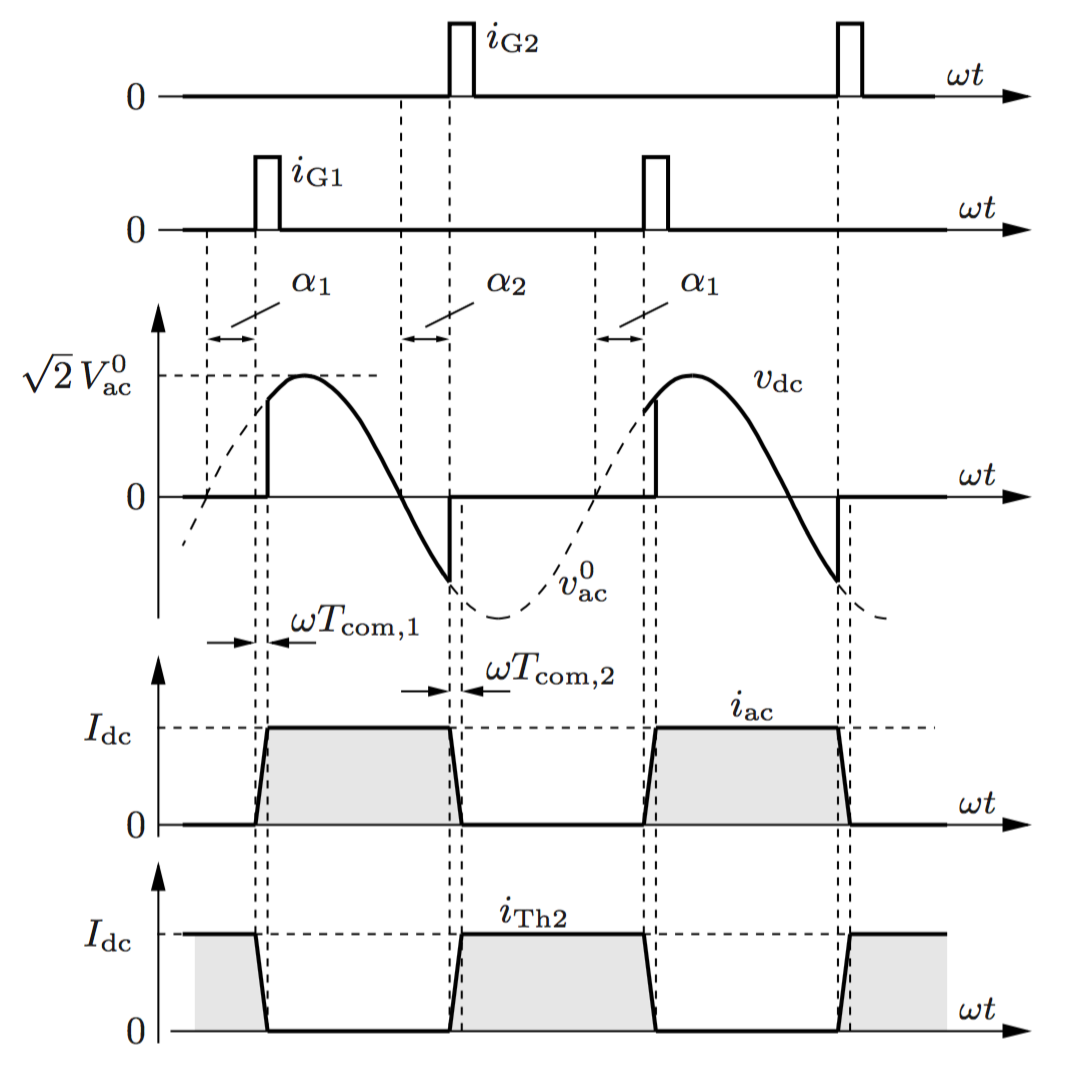
\includegraphics[scale=0.3]{ch1/4}
	\captionof{figure}{}
	\label{fig:1.4}
	\end{wrapfigure}
	Momentum in this course is noted $\vec{P}(t)$. For closed systems,
	\begin{equation}
		\frac{d\vec{P}(t)}{dt} = \sum \vec{F} = \frac{d}{dt}\int _{V(t)} \rho \vec{u}\, dV
		\label{eq:1.18}
	\end{equation}
	where $\rho \vec{u}$ is the momentum density. We will spell out the expression of the 2 members. First, the derivative, using the Reynolds transport theorem gives 
	\begin{equation}
		\frac{d\vec{P}}{dt} = \int _{V(t)} \frac{\D \rho \vec{u}}{\D t}\, dV + \oint _{S(t) = \D V(t)} \rho \vec{u} (\vec{u} \vec{n}) \, dS
	\end{equation}
	This written in indicial notation
	\begin{equation}
	\begin{aligned}
		\frac{dP_i}{dt} &= \int _{V(t)} \frac{\D \rho u_i}{\D t}\, dV + \oint _{S(t) = \D V(t)} \underbrace{\rho u_i u_j}_{tensor :\, \vec{u} \otimes \vec{u}} n_j \, dS\\
		&= \int _{V(t)} \frac{\D \rho u_i}{\D t}\, dV + \oint _{S(t) = \D V(t)} \rho (\vec{u} \otimes \vec{u}) \vec{n}\, dS 
		\end{aligned}
	\end{equation}
	and by applying Gauss theorem to the surface integral

	\begin{center}
	\begin{equation}
		\frac{d\vec{P}}{dt} = \int _{V(t)} \left[\frac{\D \rho \vec{u}}{\D t} + \nabla \rho \vec{u} \otimes \vec{u} \right] dV \qquad and \qquad \frac{dP_i}{dt} = \int _{V(t)} \left[ \frac{\D \rho u_i}{dt} + \frac{\D}{\D x_j} (\rho u_i u_j) \right] dV
	\end{equation}
	\end{center}
	
	Based on the previous forms, we can generalize this for any arbitrary function $\phi$
	\begin{equation}
	\begin{aligned}
		\frac{d}{dt} \int _{V(t)} \rho \phi\, dV  &= \int _{V(t)} \left[\frac{\D \rho \phi}{\D t} + \frac{\D}{\D x_j} \rho \phi u_j \right] dt \\
		&= \int _{V(t)} \left[ \rho \frac{\D \phi}{dt} + \phi \right. \underbrace{\left( \frac{\D \rho}{\D t} + \frac{\D \rho u_j}{\D x_j} \right)}_{= 0\ \eqref{eq:1.13}}\left. + \rho u_j\frac{\D \phi}{\D x_j} \right] dV \\
		&= \int _{V(t)} \rho \left[ \frac{\D \phi}{\D t} + u_j \frac{\D \phi}{\D x_j} \right] dV
	\end{aligned}
	\end{equation}
	Similarly to thermodynamics courses, we can introduce an extensive variable $\Phi$ and an intensive $\phi$ to have 
	\begin{center}
	\theor{
	\textbf{General relation for any arbitrary function in closed systems}
	\begin{equation}
		\frac{d\Phi }{dt} = \int _{V(t)} \left[ \frac{\D \rho \phi}{\D t} + \nabla \rho \phi \vec{u} \right] dV = \int _{V(t)} \rho \dot{\phi} \, dV
	\end{equation}
	}
	\end{center}
	For the specific case where $\Phi = \vec{P}$ and $\phi = \vec{u}$, we obtain
	\begin{equation}
		\frac{d\vec{P}}{dt} = \int _{V(t)} \rho \underbrace{\left[ \frac{\D \vec{u}}{\D t} + \vec{u} \nabla \vec{u} \right]}_{\dot{u}} dV 
		\label{eq:1.24}
	\end{equation}
	We can now express the forces applied on the system. There are 2 main classes : \\
	\begin{itemize}
		\item[•] \textbf{Distance forces (volume)} $\vec{F}_V$ : \\
		This type of force allows a body to influence another without being in contact with. 
		\begin{itemize}
			\item The most present one is gravity which is applied on each fluid particles ($d\vec{F} = dm \vec{g}$). We can imagine that there exists a force density $\vec{f}$ such that 
		\begin{equation}
			\vec{F}_V = \int _{V(t)} \vec{f} \, dV = \int _{V(t)} \rho \vec{a} \, dV
			\label{eq:1.25}
		\end{equation}
		where $\vec{a}$ is a force per unit mass, so an acceleration (gravity : $\vec{f} = \rho \vec{g}$). 
		
			\item If we have an electric material, we can talk about electromagnetic forces, which can be modelled as 
		\begin{equation}
			\vec{f} = \rho _c (\vec{E}+\vec{u}\times \vec{B}) + \vec{J}\times \vec{ B}
		\end{equation}
		where $\rho _c$ is the charge density $[C/m^3]$ and the second term is the Lorentz force. Indeed, if we have a lot of particles, we can talk of an average velocity $\vec{v}_k = \vec{u}+\vec{C}_k$, where $C_k$ is a particular velocity due to molecular agitation.  The force applied on the system is 
		\begin{equation}
			\vec{F}_k = q_k [\vec{E} + \vec{v}_k \times \vec{B}] \qquad \Leftrightarrow \qquad \underbrace{\frac{\sum \vec{F}_k}{V}}_{\rho _c} = \frac{\sum q_k}{V} (\vec{E}+\vec{u}\times \vec{B}) + \underbrace{\frac{\sum q_k \vec{C}_k}{V}}_{\vec{J}} \times \vec{B}
		\end{equation}
		Mollecules are in general neutral, but containing non-neutral regions. Fluids are essentially neutral, $\vec{F}_V = 0$ in most cases. They are called quasi-neutral fluids. Electric influenced fluids will not be considered in that course but they existence has to be known. 
		
			\item They are also entrainment and Coriolis forces in rotating frame of references. These forces due to the rotation of Earth are not considered due to the small rotative velocity, unlike pomps and turbines. \\
		\end{itemize}
		\item[•] \textbf{Contact forces (surface)} $\vec{F}_S$ : \\
		
		\begin{minipage}{0.23\textwidth}
		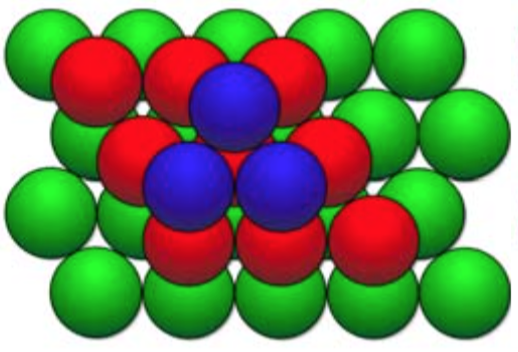
\includegraphics[scale=0.3]{ch1/5}
		\captionof{figure}{ }
		\label{fig:1.5}
		\end{minipage}
		\begin{minipage}{0.7\textwidth}
		These forces results from the contact of an internal and external fluid in regard of a region of surface $dS(t)$. We have 
		\begin{equation}
			d\vec{F}_S = \vec{T}\, dS \qquad \Rightarrow \vec{F}_S = \oint _S \vec{T}\, dS
			\label{eq:1.28}
		\end{equation}
		$\vec{T}$ is a force per unit area, a continuous function of space depending on location $\vec{x}$ and also linearly on the infinitesimal surface orientation $\vec{n}$. If $\vec{T}$ is the force per unit area for a surface element normal
		\end{minipage}
		 to the unit vector in the $j$ direction $e_j$, $\vec{T}(\vec{x}) = \vec{T}_jn_j$. \eqref{eq:1.28} becomes
		 \begin{equation}
		 \vec{F}_S = \oint _S \vec{T}_j n_j \, dS \qquad and \qquad F_{S_i} = \oint _S \underbrace{\tau _{j,i}}_{\sigma _{ji}} n_j\, dS 
		 \label{eq:1.29}
		 \end{equation}
		 where $\sigma _{ji}$ is the stress tensor. 
		\end{itemize}
		We can now take \eqref{eq:1.18} and replace the terms using \eqref{eq:1.24}, \eqref{eq:1.25} and \eqref{eq:1.29} to obtain the 
		
		\begin{center}
		\theor{\textbf{Momentum equation (integral form)}
		\begin{equation}
			\frac{dP_i}{dt} = \int _{V(t)} \left[\frac{\D \rho u_i}{\D t} + \nabla \rho u_i \vec{u} \right] dV = \int _{V(t)} \rho \dot{u}\, dV = \int _{V(t)} \rho a_i\, dV + \oint _{S(t)} \sigma _{ji} n_j \, dS
			\label{eq:1.30}
		\end{equation}
		}
		\end{center}
		We can see that $\sigma _{ji}$ and $\rho u_iu_j$ have the same mathematical nature. This is not surprising because in fact these forces result from molleculare agitation in fluids. Let's discuss it. We said that $\vec{v}_k = \vec{u} + \vec{C}_k$. Let's consider a surface element and make the hypothesis that the fluid is in rest, so the average velocity $\vec{u} = 0$. It doesn't mean that the particles are immobile, but that if all particles have the same mass (pure fluid) and if a certain number of particles are going from right to left with velocity $\vec{c}$, there are the same number of particles going from left to right with velocity $-\vec{c}$. There is no global mass flux. So for n particles going in one direction, the mass flux
		\begin{equation}
			2nm\vec{u} = nm\vec{c} + 2nm(-\vec{c}) = 0 
		\end{equation}
		To obtain the momentum in direction $x_1$, we have to multiply the mass flow in this direction by the velocity in this direction 
		\begin{equation}
			nm (\vec{c}\cdot \vec{e_1})c_1 + nm (-\vec{c_1}\cdot \vec{e_1})(-c_1) = 2nmc_1^2
		\end{equation}
		The global momentum flux traversing the unit surface is so positive going out of the volume. We need so a balance force in the opposite direction to keep the mass in. This explains the presence and nature of $\sigma _{ji}$ which is a momentum flux. \\
	Let's finally establish the differential form of the momentum equation, applying Gauss theorem to the second right side of \eqref{eq:1.30}
	\begin{equation}
		\int _{V(t)} \rho a_i\, dV + \oint _{S(t)} \sigma _{ji} n_j \, dS = \int _{V(t)} \left[ \rho a_i + \frac{\D \sigma _{ji}}{\D x_j} \right] dV
	\end{equation}
	and by considering the whole equation
	\begin{equation}
		\int _{V(t)} \left[ \frac{\D \rho u_i}{\D t} + \frac{\D \rho u_i u_j}{\D x_j} - \rho a_i - \frac{\D \sigma _{ji}}{\D x_j} \right] dV = 0 = \int _{V(t)} \left[ \rho \dot{u}_i - \rho a_i - \frac{\D \sigma _{ji}}{\D x_j} \right] dV
	\end{equation}
	and for this to be true for all systems we consider, we obtain
	\begin{center}
		\theor{\textbf{Momentum equation (differential form (1) - divergent form)}
		\begin{equation}
			\frac{\D \rho u_i}{\D t} + \frac{\D \rho u_i u_j}{\D x_j} = \rho a_i + \frac{\D \sigma _{ji}}{\D x_j} \qquad and \qquad \frac{\D \rho \vec{u}}{\D t} + \nabla \rho \vec{u}\otimes \vec{u} = \rho \vec{a} + \nabla \bar{\bar{\sigma}}
			\label{eq:1.35}
		\end{equation}
		}
		\end{center}
		
	\begin{center}
		\theor{\textbf{Momentum equation (differential form (2) - substancial form)}
		\begin{equation}
			\rho a_i + \frac{\D \sigma _{ji}}{\D x_j} = \rho \dot{u}_i \qquad and \qquad \rho \vec{a} + \nabla \bar{\bar{\sigma}} = \rho \dot{\vec{u}}
			\label{eq:1.36}
		\end{equation}
		}
		\end{center}
		
	\subsection{Angular momentum equation}
		This is a corollary of the momentum equation that states that \textit{the time rate of change of the angular momentum of a closed system is equal to the sum of the torques applied to the system.} There is no additional information except that the stress tensor should be symetric 
		\begin{equation}
			\sigma _{ji} = \sigma _{ij}
		\end{equation}
		
	\subsection{Energy equation - First principle of thermodynamics}
		If we note $\mathcal{E}$ the total energy of the system, the first principle tells that
		\begin{equation}
			\frac{d\mathcal{E}}{dt} = \dot{W} + \dot{Q}
			\label{eq:1.38}
		\end{equation}
		where $\dot{W}$ is the mechanical power provided by the forces applied on the system and $\dot{Q}$ the thermal power provided to the system. We will proceed like the previous equation expressing first the left side then the right side. If we note $E$ the total energy per unit mass, $e$ the internal energy per unit mass and $k$ the kinetic energy per unit mass (potential energy is not considered in order not to take into account power coming from potential forces)
		\begin{equation}
			\mathcal{E} = \int _{V(t)} E\, dm = \int _{V(t)} \rho E \, dV = \int _{V(t)} \rho (e+k) \, dV \qquad with \quad k = \frac{\vec{u} \vec{u}}{2}
		\end{equation}
		The time derivative of the energy using the Reynolds transport theorem, then the Gauss theorem is 
		\begin{equation}
		\begin{aligned}
			\frac{d\mathcal{E}}{dt} &= \int _{V(t)} \frac{\rho (e+k)}{dt} \, dV + \oint _{S(t)} \rho (e+k)\vec{u} \vec{n} \, dS \\
			&= \int _{V(t)} \left[\frac{\rho (e+k)}{dt} + \nabla \rho (e+k)\vec{u}  \right] dV = \int _{V(t)} \rho \dot{(e+k)}\, dV 
		\end{aligned}
		\label{eq:1.40}
		\end{equation}
		Let's now go on with with the mechanical power expression. We expressed in \eqref{eq:1.30} that there are volume and surface forces. These multiplied by the velocity and using Gauss gives 
		\begin{equation}
			\dot{W} = \int _{V(t)} \rho a_i u_i \, dV + \oint _{S(t)} \sigma _{ji} u_i n_j \, dS = \int _{V(t)} \left[ \rho a_i u_i + \frac{\D}{\D x_j}\sigma _{ji} u_i\right] dV
			\label{eq:1.41}
		\end{equation}
		\begin{wrapfigure}[6]{l}{3cm}
		\vspace{-5mm}
		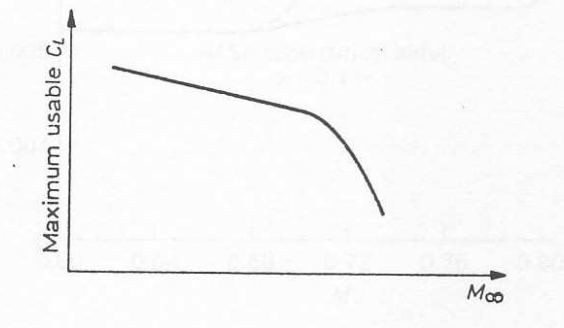
\includegraphics[scale=0.3]{ch1/6}
		\captionof{figure}{}
		\end{wrapfigure}
		For the thermal power expression, we need to introduce a new concept that is the heat flux vector $\vec{q}$ which qualifies a thermal power per unit area leaving the surface. Physically, there is only two heat transport mecanism which are radiation and conduction. Indeed, convection is a specific conduction case where the temperature gradient region becomes thinner and favorises the exchange. The thermal power is 
		\begin{equation}
			\dot{Q} =  - \oint _{S(t)} \vec{q} \vec{n} \, dS = - \int _{V(t)} \nabla \vec{q} \, dV
			\label{eq:1.42}
		\end{equation}
		Replacing the terms of \eqref{eq:1.38} by \eqref{eq:1.40}, \eqref{eq:1.41} and \eqref{eq:1.42} gives 
		\begin{center}
		\theor{
		\textbf{Total energy equation (integral form)}
		\begin{equation}
			\int _{V(t)} \frac{\rho (e+k)}{dt} \, dV + \oint _{S(t)} \rho (e+k)\vec{u} \vec{n} \, dS = \int _{V(t)} \rho \vec{a}\vec{u} \, dV + \oint _{S(t)} (\bar{\bar{\sigma}} \vec{n}) \vec{u}\, dS - \oint _{S(t)} \vec{q} \vec{n} \, dS
		\end{equation}
		}
		\end{center}
		
		The differantial form is obtained using Gauss theorem for the two sides and regrouping all the terms into one integral
		\begin{equation}
		\begin{aligned}
			&\int _{V(t)} \left[\frac{\rho (e+k)}{dt} + \nabla \rho (e+k)\vec{u} - \rho \vec{a} \vec{u} - \nabla \bar{\bar{\sigma}}\vec{u} + \nabla \vec{q} \right] dV = 0 \\
			\Leftrightarrow \qquad &\int _{V(t)} \left[\rho\dot{(e+k)} - \rho \vec{a} \vec{u} - \nabla \bar{\bar{\sigma}}\vec{u} + \nabla \vec{q} \right] dV = 0
		\end{aligned}
		\end{equation}
		
		And considering the fact that this has to be true for all systems, we obtain the two last forms
		\begin{center}
		\theor{
		\textbf{Total energy equation (differential form (1) - divergent form)}
		\begin{equation}
			\frac{\rho (e+k)}{dt} + \nabla \rho (e+k)\vec{u} = \rho \vec{a} \vec{u} + \nabla \bar{\bar{\sigma}}\vec{u} - \nabla \vec{q}
		\end{equation}
		}
		\end{center}
		\begin{center}
		\theor{
		\textbf{Total energy equation (differential form (2) - substantial form)}
		\begin{equation}
			\rho \dot{(e+k)} = \rho (\dot{e} + \dot{k}) = \rho \vec{a} \vec{u} + \nabla \bar{\bar{\sigma}}\vec{u} - \nabla \vec{q}
			\label{eq:1.46}
		\end{equation}
		}
		\end{center}
		Let's finally establish the distribution of the forces in the different energies. If we multiply \eqref{eq:1.36} by velocity $\vec{u}$ and if we observe that $\dot{k} = \frac{\dot{u}_i u_i+u_i\dot{u}_i}{2} = u_i \dot{u}_i$, we obtain 
		
		\begin{center}
		\theor{
		\textbf{Kinetic - Mechanical energy equation}
		\begin{equation}
			\vec{u}\left(\rho a_i + \frac{\D \sigma _{ji}}{\D x_j} = \rho \dot{u}_i\right) \qquad \Leftrightarrow \qquad \rho \underbrace{u_i \dot{u}_i}_{\dot{k}} = \rho u_i a_i + \frac{u_i \D\sigma _{ji}}{\D x_j}
			\label{eq:1.47}
		\end{equation}
		}
		\end{center}
		The difference between total energy \eqref{eq:1.46} and kinetic energy \eqref{eq:1.47} gives the internal energy
		
		\begin{center}
		\theor{
		\textbf{Internal energy equation}
		\begin{equation}
			\rho \dot{e} = 0 + \sigma _{ji} \frac{\D u_i}{\D x_j} - \nabla \vec{q} 
			\label{eq:1.48}
		\end{equation}
		}
		\end{center}
		We see that volume forces only contributes to the kinetic energy, heat flux only to the internal energy and the suface forces to both. 
		
	\subsection{Summary - Complementary equation}
		Let's make the inventory of the 3 substancial equations that we found. How many equations and unknowns do we have? 
	\begin{itemize}
		\item[•] In continuity equation \eqref{eq:1.17}, $\rho$ and $u_i$ are 4 unknowns in 3D. 
		\item[•] In momentum equation \eqref{eq:1.36}, $a_i$ is an external applied force so is known, $\sigma _{ji}$ consists in 6 unknowns (symetric matrix).
		\item[•] In internal energy equation \eqref{eq:1.48}, $e$ and $\vec{q}$ are 4 most unknowns. 
	\end{itemize}			
	\ \\
	The total unknowns number is 14.  The number of disponible equations is 5, 1 thanks to the energy, 1 thanks to the continuity and 3 thanks to the vectorial momentum equation. In this stage, we haven't made any assumption on the nature of the material we're considering. These equations are valid for an elastic solid as a fluid. The main difference is that solids resist to a deformation whereas fluid doesn't. But fluid resists to a rate of deformation. The way that stress tensor $\sigma _{ji}$ is related to the displacement field is called the constitutuve equations. 
	
	\subsubsection{Constitutive relations} 
		For a fluid, the stress tensor depends on the fluid rate of deformation (rate of strain). To express $\sigma _{ji}$, we have to find a quantity in the field of motion of the fluid that represents the rate of strain. If the velocity field $\vec{u}(\vec{x},t)$ was uniform, not depending on $\vec{x}$, the fluid will be moving as a bulk and there is no rate of deformation. The rate of strain must be somehow related to the velocity gradient tensor $\nabla \otimes \vec{u}$. We know that all tensors can be decomposed in an antisymetric and symetric part like 
		\begin{equation}
			\nabla \otimes \vec{u} = \frac{\D u_j}{\D x_i} = \Omega _{ji} + S _{ij} = \frac{1}{2} \left( \frac{\D u_j}{\D x_i} - \frac{\D u_i}{\D x_j} \right) + \frac{1}{2} \left( \frac{\D u_j}{\D x_i} + \frac{\D u_i}{\D x_j} \right).
		\end{equation}
		
		For a constant gradient velocity field, the velocity field is linear in the coordinates
		\begin{equation}
			u_j = \frac{\D u_j}{\D x_i}x_i = \Omega _{ji} x_i + S _{ij} x_i
			\label{eq:1.51}
		\end{equation}
		
		Let's look to the mathematical nature of the antisymetric part.  If we express using Kronecker $\delta$, we have
		\begin{equation}
			\Omega _{ji} =\frac{1}{2} \left( \frac{\D u_j}{\D x_i} - \frac{\D u_i}{\D x_j} \right) = \frac{1}{2} \delta _{kij}\delta _{kqp} \frac{\D u_p}{\D x_q} \qquad 
			with \quad \delta _{kij}\delta _{kqp} = \delta _{iq}\delta _{jp} - \delta _{ip}\delta _{jq} 
		\end{equation}
		Knowing that $(a \times b)_k = \delta _{kpq} a_p b_q$, we can introduce the \textbf{curle} (rotationnel) of velocity called vorticity $\vec{\omega}$
		\begin{equation}
			\delta _{kqp} \frac{\D u_p}{\D x_q} = (\nabla \times \vec{u})_k \qquad \Rightarrow \nabla \times \vec{u} = \vec{\omega}
		\end{equation}		 
		Let's look to the way this is linked to \eqref{eq:1.51}
		\begin{equation}
			 u_j^{AS} = \Omega _{ji}x_i = \frac{1}{2} \delta _{jki} \omega _k x_i = \frac{1}{2} (\vec{\omega} \times \vec{x})_j
			\qquad \Leftrightarrow \qquad 
			\vec{u}^{AS} = \frac{1}{2} \vec{\omega}\times \vec{x}
		\end{equation}
	 	In conclusion, we see that the antisymetric part consists in a pure rotation velocity field, a rigid body motion of angular velocity $\frac{1}{2}\vec{\omega}$ without strain. $\vec{\omega}$ is twice the angular velocity of fluid particles around themselves. The quantity representative of the fluid rate of strain can only be the symetric part of the velocity gradient tensor called the rate of strain tensor. For a fluid, $\sigma _{ij} = f(S_{ij})$. \\
	 	
	  To determine the nature of this relationship, we will assume that $\sigma _{ij} $ is a linear function of $S_{pq}$. This is called 
	\begin{center}	  
	\theor{
	  \textbf{Newton's assumption for stresses}
	  \begin{equation}
	  	\sigma _{ij} = a_{ij} + b_{ijpq} S_{pq}.
	  \end{equation}
	  }
	  \end{center}
	  In this equation, $b_{ijpq}$ is a tensor with four indices, but we know that it's symetric with respect to $pq$ and $ij$ because $S$ is symetric with respect to $pq$ and $ij$, leading to $6 \times 6 = 36$ coefficients. Symetric tensor $a_{ij}$ counts 6 coefficients, for a total of 42 coefficients. \\
	  If we assume that the fluid is \textbf{isotropic}, meaning that the fluid react in the same way whatever the sollicitation direction. For example, let's take a case of $S_{ij}$ where all coefficients are null except the $S_{11}$ term. Diagonal terms reprensent a rate of elongation/stretch while the off-diagonal terms represent an angular deformation between two perpendicular direction. The assumption means that if the rate of stress is not in 1 direction but 2, the fluid reaction will be the same. In other words, if we make a rotation of coordinates, the relation in the rotated frame of reference must be the same. In that case, the relation reduces to
	  \begin{equation}
	  	\sigma _{ij} = a \delta _{ij} + bS _{ij} + c \delta _{ij}S_{kk}
	  	\label{eq:1.55}
	  \end{equation}
	  where only 3 coefficient must be found. It is natural to think that air and water have no preferential direction unlike certain solid as wood that has a preferential direction related to the orientation of fibers. Blood or dissolved polymer chains are examples of non isotropic fluids. We will from now consider the fluid to be isotropic. \\
In \eqref{eq:1.55} $a$ is a constant that represents the stress present when the fluid is at rest. 	The surface force associated to that component is purely normal 
		\begin{equation}
			\sigma _{ij} n_j = a \delta _{ij} n_j = an_i
		\end{equation}
		This constant corresponds to the pressure exerted by the fluid at rest. Because of its application in the opposite direction to the normal, it's negative. The two other coefficients represents the 2 coefficients of viscosity
		\begin{equation}
			a = -p \qquad b = 2\mu \qquad c = \lambda
		\end{equation}
		The stress tensor equation can so be written with a pressure stress and a viscous stress part like 
		\begin{equation}
			\sigma _{ij} = -p\delta _{ij} + \tau _{ij} \qquad with \qquad \tau _{ij} = 2\mu S_{ij} + \lambda \delta _{ij} S_{kk}
			\label{eq:1.58}
		\end{equation}
	  	An alternative form to that is the following 
	  	\begin{equation}
	  		\tau _{ij} = 2 \mu \underbrace{\left( S_{ij} + \frac{1}{3} \delta _{ij} S_{kk} \right)}_{\equiv S_{ij}^S} +\underbrace{\left( \lambda + \frac{2\mu}{3} \right)}_{\equiv \mu _V} \delta _{ij} S_{kk}
	  	\end{equation}
	  	This notation is necessary to make appear the part of the strain tensor which has no trace $S_{ij}^S$, called the rate of shear. Indeed 
	  	\begin{equation}
	  		S_{ii}^S = S_{ii} - \frac{1}{3}\delta _{ii}S_{kk} = 0
	  	\end{equation}
	  	This means that $S_{ij}^S$ represents the trace less part of the rate of \textbf{strain} tensor called the sheer rate tensor. What is now $S_{kk}$ ? 
	  	\begin{equation}
	  		S_{kk} = \frac{1}{2} \left( \frac{\D u_k}{\D x_k} + \frac{\D u_k}{\D x_k} \right) = \frac{\D u_k}{\D x_k} = \nabla \vec{u}
	  	\end{equation}
	  	The divergence of the velocity is related to the rate of dilatation of the fluid, the change of volume. We decomposed the rate of strain in a part representing the deformation without change of volume (pure deformation) and another with change of volume ($\mu _V$ is the bulk viscosity). Another expression for $\tau _{ij}$ with a final net gain of 3 unknowns is 
	  	\begin{equation}
	  		\tau _{ij} = 2 \mu S_{ij}^S + \mu _V \delta _{ij} \nabla \vec{u}
	  		\label{eq:1.62}
		\end{equation}	  	 
		At this stage, we have to determine still 6 unknowns from the 9 at the beginning. 
		
	\subsubsection{Heat flux}
		We discussed about the fact that heat flux propagates using 2 physical mechanism : conduction and radiation. In the energy equation it's the divergence of the heat fluc that appears. In most application, the radiative effect does not imply heat accumulation or loss. The fluids are so transparent to radiative heat flux $\nabla \vec{q}^{rad} =0$. We only have conduction and the Fourier law says that 
		\begin{equation}
			\vec{q} \propto \nabla T = d\nabla T = -\kappa \nabla T \qquad \Leftrightarrow \qquad q_i = -\kappa \frac{\D T}{\D x_i}
		\end{equation}
	The negative sign comes from the fact that heat goes from hot to cold (decrease of T). We have a net gain of 1 unknown with this equation. 
	
	\subsubsection{Thermodynamics}
		At this stage, we are using 4 thermodynamics intensive variables which are $\rho, e, p, T$. We know that for a single phase fluid, the variance is 2, meaning that we can use 2 thermodynamics equations of state (EoS) relating them. For example, for a alorically and thermally perfect gas, we will have 
		\begin{equation}
			p = \rho R T \qquad and \qquad e = c_v T
		\end{equation}		 
		We have a net gain of 2 unknows, so there remains 2 unknowns.  
		
	\subsubsection{Transport coefficients}
		The remaining variables are the shear viscosity $\mu$, the bulk viscosity $\mu _V$ and thermal conductivity $\kappa$. These are functions of the thermodynamic state. For example for gases we have the relations 
		\begin{equation}
			\mu = f(T) \qquad and \qquad Pr = \frac{\mu c_p}{\kappa} = cst \Leftrightarrow \kappa = \frac{\mu (T) c_p (T)}{Pr}
		\end{equation}
		The bulk viscosity is more difficult to determine, but it can be shown that for monoatomic gases (no internal degres of freedom) $\mu _V=0$. For diatomic gases it's much more delcate to measure, but it has been shown that for many flows, the flows is insensitive to the variation of value of bulk viscosity. In fact, for fluids without divergence of velocity, we don't care about $\mu _V$ because there is no variation of volume  \eqref{eq:1.62}. We will so make the following assumption
		\begin{center}
		\theor{\textbf{Stokes assumption}
		\begin{equation}
			\mu _V = 0 \quad \mbox{even for other gases}.
		\end{equation}
		}
		\end{center}
		 We're done, we have as many equations as variables. We mentioned the first principle of thermodynamics but not the second. Let's analyse that. 
		 
		\subsubsection{Second principle of thermodynamics}
			We will reuse the internal energy equation \eqref{eq:1.48}, replace $\sigma _{ij}$ by it's expression in \eqref{eq:1.58} and use the fact that $\frac{\D u_i}{\D x_j} = \Omega _{ij} + S_{ij}$
			\begin{equation}
				\rho \dot{e} = \sigma _{ij} \frac{\D u_i}{\D x_j} - \frac{\D q_i}{\D x_i} = -p \delta _{ij} \frac{\D u_i}{\D x_j} + (2\mu S_{ij}^S + \mu _V \delta _{ij} \nabla \vec{u})(S_{ij}+\cancel{\Omega _{ij}}) - \frac{\D q_i}{\D x_i}
			\end{equation}
			where $\Omega _{ij}$ doesn't contribute because the contraction of the symetric tensor by the antisymetric tensor is equal to 0.  We have the relation 
			\begin{equation}
			S_{ij}^S = S_{ij}-\frac{1}{3}\delta _{ij}\nabla \vec{u} \qquad \Leftrightarrow \qquad S_{ij} = S_{ij}^S + \frac{1}{3}\delta _{ij}\nabla \vec{u}
	  		\end{equation}
	  		Combined to the fact that $\delta _{ij} \frac{\D u_i}{\D x_j} = \frac{\D u_i}{\D x_i} = \nabla \vec{u}$, we obtain
	  		\begin{equation}
	  			\rho \dot{e} = -p \nabla \vec{u} + (2\mu S_{ij}^S + \mu _V \delta _{ij} \nabla \vec{u})\left( S_{ij}^S + \frac{1}{3}\delta _{ij}\nabla \vec{u}\right) - \nabla \vec{q}
	  		\end{equation}
	  		The mass conservation equation tells us that we can write the divergence as 
	  		\begin{equation}
	  			\dot{\rho} + \rho \nabla \vec{u} = 0 \qquad \Leftrightarrow \qquad \nabla \vec{u} = -\frac{\dot{\rho}}{\rho} = -\rho \left( \frac{\dot{\rho}}{\rho ^2}\right) = \rho \dot{\left( \frac{1}{\rho}\right)} = \rho \dot{v}
	  		\end{equation}
	  		If we replace the divergence in the previous equation, we have
	  		\begin{equation}
	  			\rho \dot{e} = -\rho p \dot{v} + (2\mu S_{ij}^S + \mu _V \delta _{ij} \nabla \vec{u})\left(S_{ij}^S + \frac{1}{3}\delta _{ij}\nabla \vec{u}\right) - \nabla \vec{q}
	  		\end{equation}
	  		The first term here looks like the reversible work $-pdv$ in thermodynamics and is so the reversible contribution to the internal energy. Let's make this appear by bringing this to the left side. We make appear $\rho [\dot{e} + p\dot{v}]$, but we have the famous Gibbs relation $de = Tds - pdv \Leftrightarrow \dot{e} = T\dot{s}-p\dot{v}$. We have now 
	  		\begin{equation}
	  			\rho \dot{s} = \frac{(2\mu S_{ij}^S + \mu _V \delta _{ij} \nabla \vec{u})\left(S_{ij}^S + \frac{1}{3}\delta _{ij}\nabla \vec{u}\right)}{T} - \frac{\nabla \vec{q}}{T}
	  			\label{eq:1.72}
	  		\end{equation}
	  		If we remind the relation we demonstrated before for any variable $\dot{\Phi} = \int _V \rho \dot{\phi} dV$, we can make the analogy here to say that when this is integrated over a volume, it gives the time rate of change of the entropy of the closed system that's initially inside this volume. We have to identify the reversible part in this equation. We know that the reversible entropy rate of exchange for a uniform system and its integral over a closed surface is given by
	  		\begin{equation}
	  			\frac{\vec{q}dS}{T} \qquad \Rightarrow \qquad \oint _S \frac{\vec{q}}{T}(-\vec{n})\, dS = -\int _V \nabla \frac{\vec{q}}{T} \, dV.
			\end{equation}	  		 
			We see that we have to make appear a this in the last equation. But we know that
			\begin{equation}
				\frac{\nabla \vec{q}}{T} = \nabla \frac{\vec{q}}{T} - \vec{q} \nabla \left(\frac{1}{T} \right) = \nabla \frac{\vec{q}}{T} + \vec{q} \frac{\nabla T}{T^2}
			\end{equation}
			And by introducing this into the relation \eqref{eq:1.72}, we make appear the reversible entropy rate of exchange
			\begin{equation}
				\rho \dot{s} = -\nabla \frac{\vec{q}}{T} - \frac{\vec{q}\nabla T}{T^2} + \frac{(2\mu S_{ij}^S + \mu _V \delta _{ij} \nabla \vec{u})\left(S_{ij}^S + \frac{1}{3}\delta _{ij}\nabla \vec{u}\right)}{T}
			\end{equation}
			We also know that $\vec{q} = -\kappa \nabla T$, making appear $(\nabla T)^2$
			\begin{equation}
				\rho \dot{s} = -\nabla \frac{\vec{q}}{T} + \frac{\nabla T\nabla T}{T^2} + \frac{(2\mu S_{ij}^S + \mu _V \delta _{ij} \nabla \vec{u})\left(S_{ij}^S + \frac{1}{3}\delta _{ij}\nabla \vec{u}\right)}{T}
			\end{equation}
			If we imagine a fluid at rest with only a heat exchange operating on it, the third term $=0$, the first term is reversible so anyway the sign and the second term must be positive. This implies $\kappa \geq 0$ due to the square of the other varaibles (the heat has to go from hot to cold). Let's expand the third term
			\begin{equation}
				\rho \dot{s} = -\nabla \frac{\vec{q}}{T} + \frac{\nabla T\nabla T}{T^2} + \frac{1}{T}\left[ 2\mu S_{ij}^S S_{ij}^S + \cancel{\mu _V \nabla \vec{u} \delta _{ij} S_{ij}^S} + \cancel{2\mu S_{ij}^S \frac{\delta _{ij}}{3} \nabla \vec{u}} + \mu _V \frac{\delta _{ij}\delta _{ij}}{3}(\nabla \vec{u})^2  \right]			
			\end{equation}			 
			In this last equation, the second and third terms are nul because $S_{ii}^S=0$. Let's imagine that we have a fluid with only dilation and no shear $S_{ij}^S$, the last term must be positive and so $\mu _V$ has to be positive ($\geq 0$). In the other hand, for the first term, we have a quadratic form (sum of squares $\geq 0$), so $\mu$ has to be positive. To verify the second principle, we have to verify these 3 inequalities. In fluid mechanics, we don't have to worry about the second principle, it's built in the equations as long as the transport coefficient are positive.  
			
	\subsection{Boundary conditions}
		We have now to establish the boundary conditions which makes the difference between the flow cases. First of all, we have two main categories of flows : 
		\begin{itemize}
			\item[•] \textbf{External flows} (unbounded domain)\\
				For example, a flow over a wing, assuming that atmosphere extends to infinity. In that case we have far field boundary conditions, what happens far from the body ($u\rightarrow u_\infty, p\rightarrow p_\infty, T\rightarrow T_\infty)$. 
			
			\item[•] \textbf{Internal flows} (bounded domain)\\
				For example, a flow in a pipe or a fluid in a rotating machine like a pump. In that case we don't have the far field conditions but the inlet and outlet boundary conditions but this problem is not discussed here. 
		\end{itemize}
		
		\subsubsection{Solid surfaces}
			In both case we have solid surfaces, we have to make a distinction. We wrote the equation for the general case of a viscous flow, but there is flows where the viscous stresses can be neglected (not $=0$ !) leading to what we call the \textbf{inviscid flows}. Let's analyse the two cases. 
			
		\subsubsection{Viscous flows}
			Viiscosity is associated to the exchange of momentum between neighboring fluid layers due to molecular agitation. If we have a molecule coming from a low velocity region to a high velocity region, it slows down the molecule there and inversely. The same occurs when a fluid particle enter in contact with solid surfaces, it exchange momentum. The result is that velocity and temperature fields must be continuous 
			\begin{equation}
				\vec{u}_{fluid} = \vec{u}_{wall} \qquad and \qquad T_{fluid} = T_{wall}
			\end{equation}
			In particular, for a surface at rest, the fluid must be at rest on the solid surface as well. This is called the \textbf{no-slip condition}. 
		
		\subsubsection{Inviscid flows} 
			For inviscid flows, this mecanism doesn't exist, the fluid may slip. The boundary condition is that the fluid can't go throw the solid
			\begin{equation}
				\vec{u}_{fluid}\vec{n} = \vec{u}_{wall}\vec{n}
			\end{equation}
			This is called the \textbf{slip/no penetration condition}. The previous condition is stronger because in fact $\vec{u} = \vec{u}_n\vec{n}+\vec{u}_t$ includes the tangential condition too. 
			
\section{Special cases}
	\subsection{General case}
		The generale equations are the following : 
		\begin{itemize}
			\item[•] Mass conservation equation 
			\begin{equation}
				\dot{\rho} + \rho \nabla \vec{u} = 0 
			\end{equation}
			
			\item[•] Momentum equation
			\begin{equation}
				\rho \dot{\vec{u}} = - \nabla p + \nabla \bar{\bar{\tau}} + \rho \vec{F}
			\end{equation}
			
			\item[•] Energy equation
			\begin{equation}
				\rho \dot{e} = - p \nabla \vec{u} + \underbrace{\bar{\bar{u}} .. \nabla \otimes \vec{u}}_{\epsilon _V} - \nabla \vec{q}
			\end{equation}
			where $\nabla \otimes \vec{u}$ can be replace by the symetric part, rate of strain tensor $\bar{\bar{S}}$ and $\epsilon _V$ is the viscous dissipation. \\
			
			\item[•] Constituve relation
			\begin{equation}
			\begin{aligned}
				\tau _{ij} &= 2\mu \left( S _{ij} - \frac{1}{3}\delta_{ij}\nabla \vec{u} \right) + \mu _V S_{ij}\nabla \vec{u}\\
				&= \mu \left( \frac{\D u_i}{\D x_j} + \frac{\D u_j}{\D x_i} - \frac{2}{3}\delta _{ij}\nabla \vec{u} \right) + \mu _V S_{ij}\nabla \vec{u}
			\end{aligned}
			\label{eq:1.83}
			\end{equation}
			
			\item[•] Conductive heat flux 
			\begin{equation}
				\vec{q} = -\kappa \nabla T
			\end{equation}
		\end{itemize}
		
	\subsection{Steady flow} 
		This is caracterized by the fact that $\frac{\D }{\D t} = 0$ and implies for example that 
		\begin{equation}
			\dot{\rho} = \frac{\D \rho}{\D t} + \vec{u} \nabla \rho = \vec{u} \nabla \rho
		\end{equation}
		and for the others. 
		
	\subsection{Inviscid flows}
		They are defined as flows in which vicous stresses and conduction heat flux can be neglected.  We are talking about flows and not fluids because there is no fluid with $\mu = 0$ or $\kappa = 0$. This happens for superfluids but we don't care. When we look at the fluid properties tables, in SI units, water and air have very small $\mu$ but we can't say that there are negligible because it depends on the system of refference used. If something is negligible  it is with respect to something else. Let's start with the viscous stresses. Momentum equation can be written as 
		\begin{equation}
			\rho \dot{\vec{u}} = \frac{\D \rho}{\D t} + \nabla \rho \vec{u} \otimes \vec{u} = -\nabla p + \nabla \bar{\bar{\tau}} + \rho \bar{F}
		\end{equation}
		where the viscous stress tensor is a tensor as the momentum flux tensor. They correspond to the same physical phenomenon but at different scales, the viscous stress tensor is due to the molecular agitation whereas the momentum flux tensor is for the macroscopic scale, the average scale. So it makes sense to compare the order of magnitude of the two ones. \\
		
		\begin{wrapfigure}[6]{l}{4cm}
		\vspace{-8mm}
		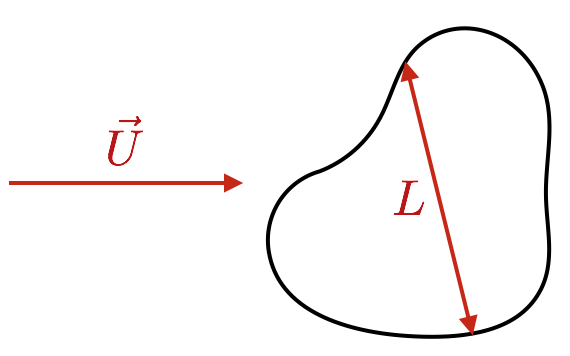
\includegraphics[scale=0.38]{ch1/7}
		\captionof{figure}{}
		\end{wrapfigure}
		Let's consider a fluid flows of far field velocity $\vec{U}$ around a solid body of characteristic lenght $L$, if we consider the momentum flux tensor, we know that the velocity around the body will vary between 0 and $U$ so the order of magnitude will be $\theta (\rho U^2)$. What about $\tau$? We see that in \eqref{eq:1.83} appears the velocity gradient, derivative. What is the order of magnitude of the derivative of a function?  
		
		\begin{wrapfigure}[8]{l}{3.5cm}
		\vspace{-5mm}
		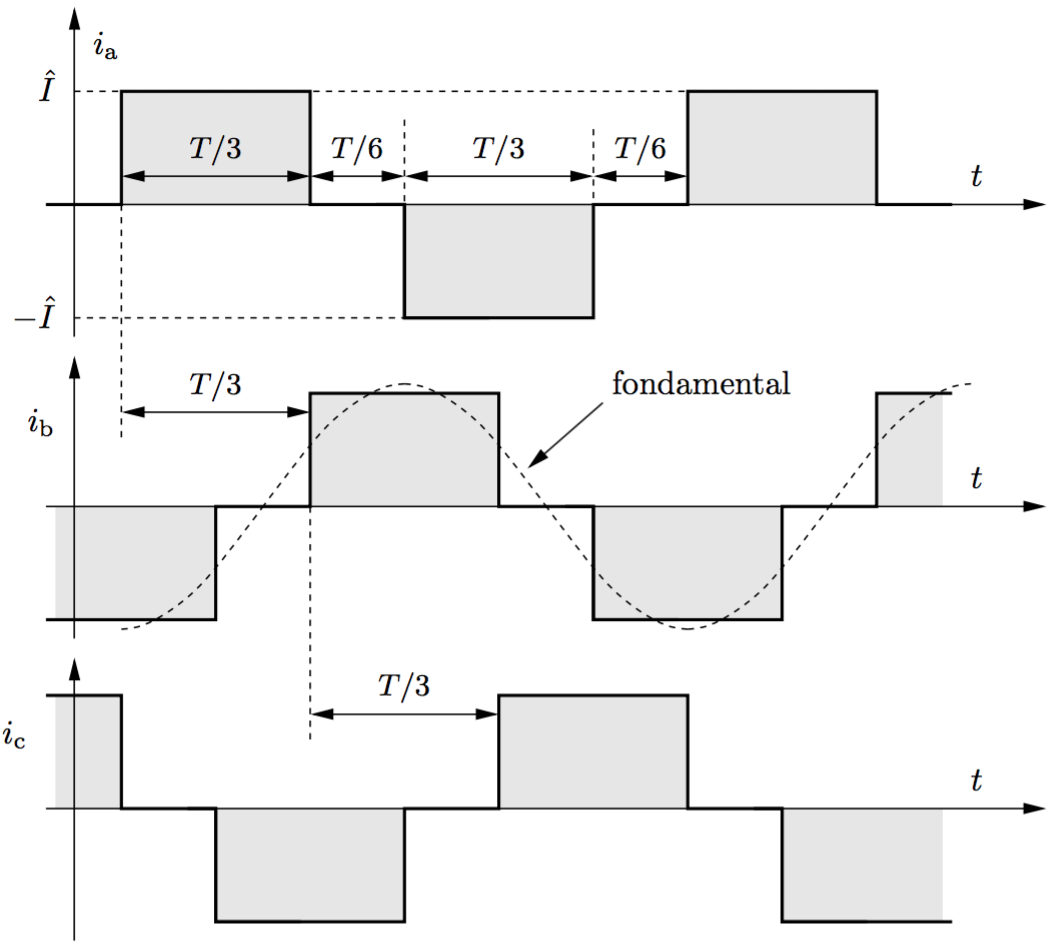
\includegraphics[scale=0.5]{ch1/8}
		\captionof{figure}{}
		\label{fig:1.8}
		\end{wrapfigure}
		Let's consider a function $f(x)$ represented on \autoref{fig:1.8}. If the function is smooth, so if the function doesn't vary much in the interval, its derivative keeps a constant order of magnitude in the integral. We see it in the figure, the slope varies between $a$ and $b$, can be twice the slope at the center but keeps the same order of magnitude. So for a smooth function, the order of magnitude of $f'$ remains the same over the interval $f' = \theta \left(\frac{\Delta f}{\Delta x}\right)$. Let's use this to have an approximation for the velocity gradient tensor 
		\begin{equation}
			\nabla \otimes \vec{u} = \theta \left( \frac{U}{L} \right) \qquad \Rightarrow \bar{\bar{\tau}} = \theta \left( \mu \frac{U}{L} \right)
		\end{equation}
		The relative order of magnitude of viscous stresses with respect to momentum flow is 
		\begin{equation}
			\frac{\mu \frac{\cancel{U}}{L}}{\rho U^{\cancel{2}}} = \frac{\mu}{\rho UL} = \frac{1}{Re_L}
		\end{equation}
		We conclude that viscous stresses can be neglected in the case of high Reynolds number. \\
		
		\begin{wrapfigure}[7]{r}{3.5cm}
		\vspace{-8mm}
		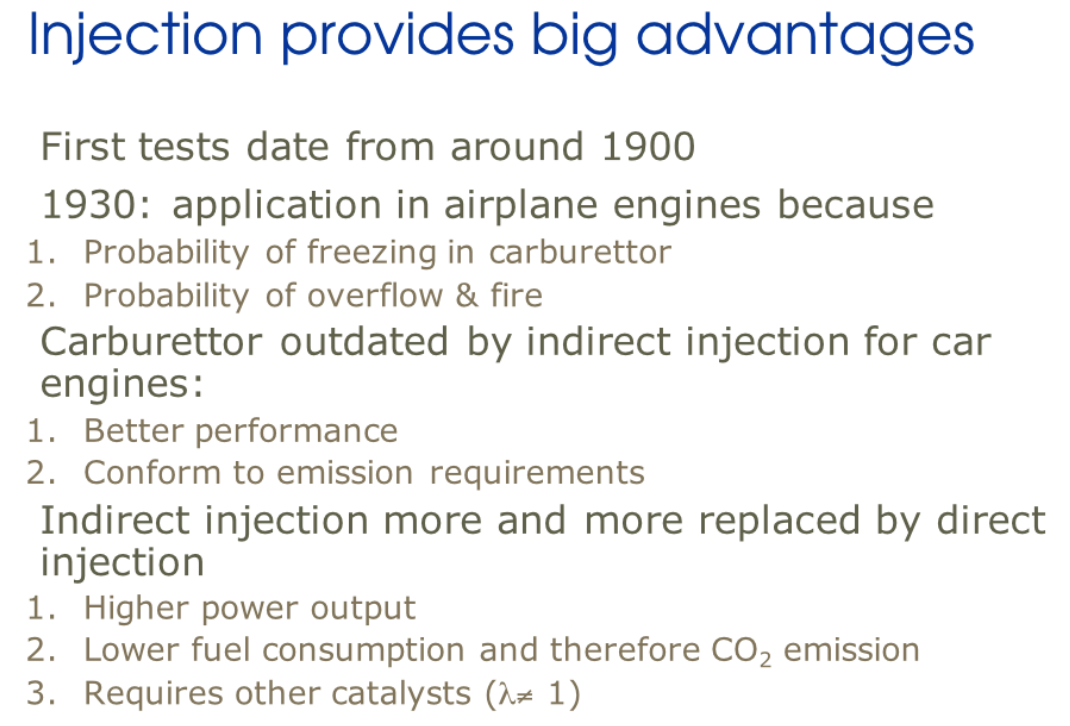
\includegraphics[scale=0.53]{ch1/9}
		\captionof{figure}{}
		\label{fig:1.9}
		\end{wrapfigure}
		Now we have to verify the assumption that velocity is a smooth function of the coordinates. Examples of not smooth functions are represented on \autoref{fig:1.9} where the green curve is smooth close to the limits but not smooth in a small interval and the yellow one is a periodic function with the characteristic wave length. In these cases, $\Delta x$ is not the appropriate length scale to determine the order of magnitude of the derivative. \\\\\\

		\begin{wrapfigure}[6]{l}{4cm}
		\vspace{-15mm}
		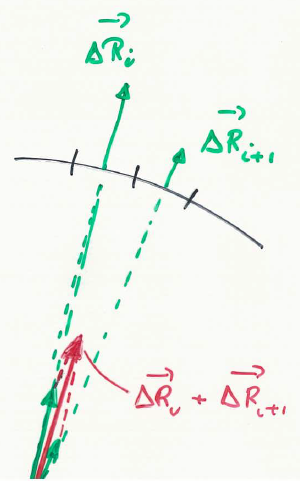
\includegraphics[scale=0.35]{ch1/10}
		\captionof{figure}{}
		\label{fig:1.10}
		\end{wrapfigure}
		Now what about the velocity field? Let's assume that velocity is smooth and the fluid inviscid, the boundary conditions to respect are the slip conditions. But we know that $\mu$ is not strictly 0, so the velocity must be 0 at the wall and therefore, there exists an area of rapidly changing velocity close to the wall. 
%%%%%%%%%%%%%%%%%%%%%%%%%%%%%%%%%%%%%
% Ch2 : Les liaisons interatomiques %
%%%%%%%%%%%%%%%%%%%%%%%%%%%%%%%%%%%%%

\chapter{Liaisons interatomiques}
\section{La liaison}
Le but des liaisons est de remplir la couche de valence et de se rapprocher au plus de la configuration des gaz rares. L'existence de composés polyatomiques stables implique que les atomes soient capable de former des agrégats dont \textbf{l'énergie est plus faible que s'ils étaient isolés}. Les types de liaison dépendent de l'agencement des électrons de valence et sont au nombre de 4 : \\

\begin{itemize}
	\item[•] la liaison ionique
	\item[•] la liaison covalente
	\item[•] la liaison métallique
	\item[•] les liaisons secondaires hydrogène et de Vander Waals. \\
\end{itemize}
	
Les 3 premières sont des liaisons fortes alors que les dernières sont plus faibles. Soulignons que, le plus souvent, la liaison des atomes dans un solide présente un caractère mixte associant des contributions simultanées de plusieurs types liaisons chimiques.
	
\section{La liaison ionique, opportunisme individualiste}
Type de liaison qui détermine la cohésion des solides constitués de l'association d'atomes possédant des affinités électronique très différentes. Prenons l'exemple du sel de cuisine $NaCl$ et regardons ce qui se passe d'un point de vue énergétique. Tout d'abord, l'énergie de première ionisation de $Na$ et l'affinité électronique (énergie libéré lorsqu'un électron est capté) de $Cl$ sont
\begin{equation}
	E_{ion}\, Na= 5.14 \, eV \qquad et \qquad \mbox{Aff.élec } Cl = 4.02 \, eV 
\end{equation}	 
ce qui veut dire qu'il faut $U_i = 1.12\, eV$ pour séparer $NaCl$ en $Na^++Cl^-$. Il faut encore tenir compte de la force électrostatique $F$ entre les deux ions de charges différentes. Quand un ion se rapproche depuis l'infini, 
\begin{equation}
	U_a = \int _\infty ^r F_{attr} \, dr= \int _\infty ^r \frac{q^2}{4\pi \epsilon _0 r^2} \, dr = -\frac{q^2}{4\pi \epsilon _0 r}
\end{equation}
Le signe négatif de cette énergie traduit le fait que les ions ont tendance à se rapprocher. Cependant, à très petite distance, les cortèges électroniques commencent à se superposer et une forte répulsion apparaît selon 
\begin{equation}
	U_r = \frac{B}{r^n}
\end{equation}
\begin{wrapfigure}[5]{l}{6.5cm}
	\vspace{-5mm}
	\includegraphics[scale=0.6]{ch2/1}
\end{wrapfigure}
La somme de toutes ces contributions donne la courbe d'énergie potentielle suivante. 
A SUIVRE
\chapter{Traction - Compression}
\section{Traction}
	\subsection{Méthode cinématique}
	\begin{wrapfigure}[8]{r}{6.5cm}
	\vspace{-5mm}
	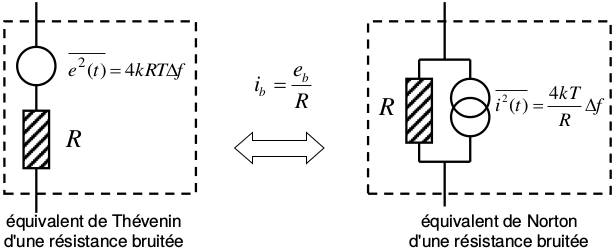
\includegraphics[scale=0.4]{ch3/image1.png}
	\captionof{figure}{ }
	\end{wrapfigure}
	Nous allons ici utiliser la méthode cinématique de sorte que les équations 
	de compatibilité soient satisfaites lors de l'obtention de notre relation 
	contrainte $\leftrightarrow N$. Il faut donc postuler un champ de 
	déplacement :
	\begin{equation}
	u = u_0(x),\qquad v=0,\qquad w=0.
	\end{equation}
	On considère un déplacement axial $u$, uniquement selon $x$ : ne varie 
	pas selon $x$ et $y$ et constante dans toute la section : une section 
	transversale plane, reste plane\footnote{hypothèse de Bernoulli (1694) :
	les sections droites initialement planes et perpendiculaires à l'axe le 
	restent dans la configuration déformée}.
	
	\subsection{Déplacements - Déformations - Contraintes}
		\subsubsection{Déformations}
		Maintenant que nous avons notre déplacement, il faut s'intéresser 
		aux déformations :
		\begin{equation}
		a_{ij} = \frac{1}{2}\left(\dfrac{\partial u_i}{\partial x_j}+\dfrac{
		\partial u_j}{\partial x_i}\right)
		\end{equation}
		De par notre champ, $\epsilon_x$ est constant dans la section 
		transversale et les autres composantes sont nulles :
		\begin{equation}
		\epsilon_x = \dfrac{\partial u_0}{\partial x}
		\end{equation}
		
		\subsubsection{Contraintes}
		On utilise pour ça la loi de Hooke $ \sigma_x = E\epsilon_x$. Notons 
		que si $E$ est constant, $\sigma_x$ l'est dans la section transversale.
		On néglige les composantes de Poisson.
		
	\subsection{Éléments de réduction : section homogène}
	La suite de notre méthode demande le calcul des éléments de réductions. 
	Supposons que l'on ai une section homogène de sorte que $E$ soit constant. 
	Dès lors, $\sigma_x$ est également constant. Pour la normale, c'est immédiat :
	\begin{equation}
	N = \int_A \sigma_x\ dA \qquad\Longrightarrow\qquad N = \sigma_xA
	\end{equation}
	En raison de notre champ uniquement selon $x$, les résultantes en $y$ et $z$ 
	sont nulles, de même pour le moment selon $x$\\
		\begin{wrapfigure}[7]{l}{6.5cm}
	\vspace{-5mm}
	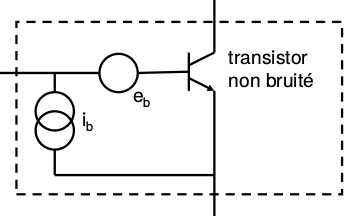
\includegraphics[scale=0.45]{ch3/image2.png}
	\captionof{figure}{ }
	\end{wrapfigure}
	\begin{equation}
	\begin{array}{ll}
	R_y = \int_A \tau_{xy}\ dA &\Longrightarrow T_y = 0\\
	\text{Similairement : }&\Longrightarrow T_z = 0\\
	C_x = \int_A (\tau_{xz}y-\tau_{xy}z)\ dA &\Longrightarrow M_x = 0
	\end{array}
	\end{equation}
	Pour le moment selon $y$ (et similairement pour $z$) nous avons :
	\begin{equation}
	C_y = \int_A \sigma_xz\ dA\qquad\Longrightarrow\qquad C_y =  \sigma_x
	\int_A z\ dA
	\end{equation}
	Si l'origine des axes est le \textbf{centre géométrique}\footnote{Centre 
	de "gravité" sans masse.} défini tel que 
	\begin{equation}
	\int_A y\ dA = 0,\qquad \int_A z\ dA = 0.
	\end{equation}
	ALors, $M_y$ et $M_z$ sont nuls.
	
		\subsubsection{En résumé}
		La poutre est uniquement soumise à un effort \textbf{normal} (et pas 
		un fléchissant). Pour une poutre de section homogène ($E$ constant), 
		nous avons une distribution uniforme de la contrainte axiale 
		\begin{equation}
		\sigma_x = \dfrac{aN}{A}
		\end{equation}
		Pour une poutre homogène à effort normal constant ($N$ constant) :
		\begin{equation}
		\epsilon_x = \dfrac{\Delta L}{L}\qquad\text{où}\quad \Delta L = 
		\dfrac{NL}{EA}
		\end{equation}
		L'hypothèse de Bernoulli est une hypothèse cinématique (\textit{Les 
		sections droites initialement planes et perpendiculaires à l'axe le
		restent dans la configuration déformée.}) et ne fait donc \textbf{pas} 
		intervenir les propriétés physiques du matériau.\\
		\danger Il n'y aura traction sans flexion \textbf{que si} les moments 
		des contraintes axiales sont nuls !
		
		
	\subsection{Éléments de réduction : section non homogène}		
	Si $E \neq\ cste$, les relations générales restent inchangées tant que 
	$E$ n'apparaît pas explicitement. Dès qu'il apparaît :
	\begin{equation}
	\sigma_x(x,y,z) = E(x,y,z)\epsilon_x(x)
	\end{equation}
	La répartition de $\sigma_x$ dans une section transversale ($x =\ cste$) 
	est dès lors donné par 
	\begin{equation}
	\sigma_x(y,z) = E(y,z)\epsilon_x
	\end{equation}
	Au niveau des éléments de réduction $R_{y,z}, M_{x,y,z}$ restent inchangés 
	(nuls\footnote{Si l'origine des axes est le centre géométrique!}). Par contre, 
	$N$ n'a plus la même expression, $\sigma_x$ n'étant plus constant.\\
	\textsc{Exemple} : slide 15-16.
	
\section{Les treillis articulés}
	\subsection{Hypothèses}
	Deux hypothèses sont d'application :
	\begin{enumerate}
	\item Il s'agit d'un ensemble de poutres rectilignes assemblées par des 
	nœuds articulés ne transmettant pas de couple (On peut tourner librement 
	l’extrémité)
	\item Les forces extérieures sont appliquées uniquement aux nœuds
	\end{enumerate}
	
	\subsection{Équilibre d'une poutre}
	Dans ce cas-ci, on ne dira pas "poutre" mais \textit{barre}. Celle-ci est 
	uniquement soumise à un effort normal $N$. Ses équations d'équilibres 
	s'obtiennent on ne peut plus facilement\\
	\begin{wrapfigure}[6]{l}{7.5cm}
	\vspace{-8mm}
	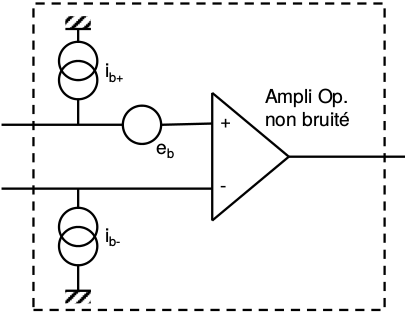
\includegraphics[scale=0.4]{ch3/image3.png}
	\captionof{figure}{ }
	\end{wrapfigure}
	\begin{equation}
	\left\{\begin{array}{ll}
	F_{xA} + F_{xB} &=0\\
	F_{yA} + F_{yB} &= 0\\
	LF_{yB} &=0
	\end{array}\right.
	\end{equation}\ \\
	
	
	\subsection{Équilibre des nœuds}
	\begin{wrapfigure}[7]{r}{6.5cm}
	\vspace{-4mm}
	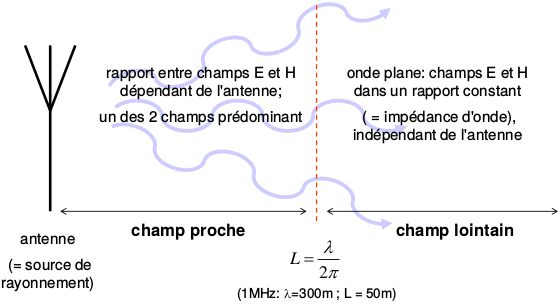
\includegraphics[scale=0.4]{ch3/image4.png}
	\captionof{figure}{ }
	\end{wrapfigure}
		Encore une fois rien de difficile, la méthode est systématique :
	\begin{itemize}
	\item[$\bullet$] Isoler un nœud en coupant les barres qui y aboutissent
	\item[$\bullet$] Appliquer les efforts normaux et les efforts extérieurs
	\item[$\bullet$] Écrire les équations d’équilibre du nœud
	\end{itemize}
	
	\subsection{Structure isostatique ?}
	La condition d'isostaticité est que le nombre d'inconnues statiques soit 
	égal au nombre d'équations d'équilibres. Nous avons :
	\begin{itemize}
	\item[$\bullet$] Nombre de barres : $b \rightarrow b$ efforts normaux 
	inconnus
	\item[$\bullet$] Nombre de RDL : $R \rightarrow R$ composantes de réactions 
	inconnues
	\item[$\bullet$] Nombre de nœuds : $n\rightarrow 2b$ équations d'équilibres 
	en 2D
	\end{itemize}
	Une structure est isostatique si (CN mais pas CNS) :
	\begin{equation}
	b + R = 2n
	\end{equation}
	\newpage
	
	\subsection{Coupe de Ritter}
		\subsubsection{Principe}
	\begin{wrapfigure}[7]{r}{7cm}
	\vspace{-4mm}
	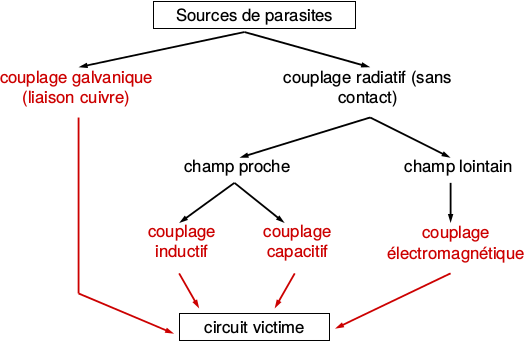
\includegraphics[scale=0.4]{ch3/image5.png}
	\captionof{figure}{ }
	\end{wrapfigure}
		On cherche à calculer l'effort normal dans une barre. On va
		\begin{itemize}
		\item[$\bullet$] Couper la structure en deux parties \textbf{disjointes}
		\item[$\bullet$] Écrire l'équilibre d'une des parties
		\item[$\bullet$] S'arranger que cet effort normal soit la seule inconnue
		\end{itemize}
		Les slides 24-25 montrent comment appliquer cette méthode.
		
	\subsection{Quelques nœuds particuliers}
	Certains nœuds particuliers permettent de gagner du temps dans les calculs.
	\begin{center}
	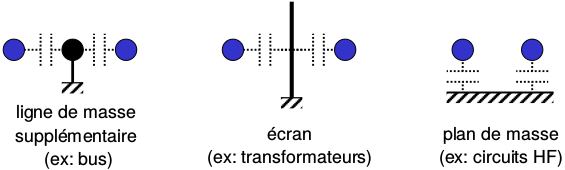
\includegraphics[scale=0.5]{ch3/image6.png}
	\captionof{table}{ }
	\end{center}
	
	
		\subsubsection{Barres à efforts nuls}
		\begin{wrapfigure}[9]{l}{7cm}
		\vspace{-6mm}
		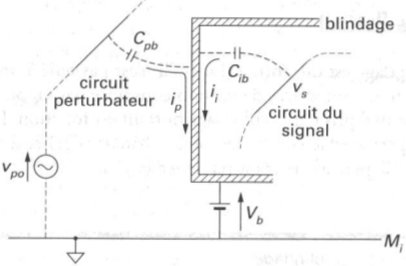
\includegraphics[scale=0.4]{ch3/image7.png}
		\captionof{figure}{ }
		\end{wrapfigure}
		En appliquant ce magnifique tableau et en l'appliquant sur la figure 
		ci-dessous, je peux déjà affirmer que pleins d'efforts normaux seront 
		nuls avant même de commencer à faire des calculs et donc gagner du 
		temps (qui, au vu de la longueur de l'examen peut être précieux).\\
		Notons que la barre du bas doit forcément être en traction, sans quoi 
		elle se "barrerait" (pfpfpf) avec le rouleau. 
		
	\subsection{Dilatation thermique}
	Il peut y avoir déformation axiale du à une élévation $\Delta T$ de la 
	température, déformation donnée par $\epsilon_{th} = \alpha\Delta T$. \\
	Si la structure est isostatique, elle est librement dilatable (car pas de 
	$T$ dans les équations d'équilibres) et son allongement est 
	\begin{equation}
	\Delta L_{th} = L\epsilon_{th} : L\alpha\Delta T
	\end{equation}
	Si la dilatation est empêchée, cela provoque un effort normal
	\begin{equation}
	N_{th} = -EA\epsilon_{th}\qquad\text{ou}\qquad N_{th} = -EA\alpha \Delta T
	\end{equation}
\chapter{La machine à courant continu}
Ces machines ne sont plus utilisées comme génératrices de puissances 
mais leurs capacité de réglage de vitesse nous pousse à les étudier. 
\textbf{Dynamo} est le nom donné à une génératrice à courant continu.

\section{Génération d'une tension continue}
	\subsection{Effet d'un collecteur}
	Pour avoir une f.e.m. continue, il faut 
	\begin{enumerate}
	\item Un collecteur
	\item Augmenter le nombre de conducteurs actifs
	\end{enumerate}
	Le \textbf{collecteur} est un commutateur ayant pour but de 
	redresser la f.e.m. alternative\footnote{"En électrotechnique, 
	un collecteur commutateur rotatif est un organe permettant de 
	créer 	une connexion électrique entre une partie fixe (stator) 
	et une 	partie tournante (rotor), avec une fonction de 
	commutation pendant la rotation. On trouve ce genre de 
	collecteur dans les machines à courant continu et les moteurs 
	électriques universels.".}.\\
	\begin{wrapfigure}[10]{l}{8.2cm}
	\vspace{-5mm}
	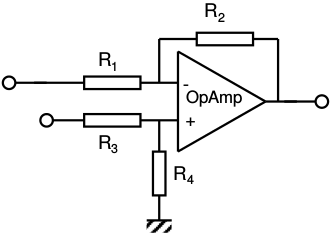
\includegraphics[scale=0.34]{ch4/image1.png}
	\captionof{figure}{ }
	\end{wrapfigure}
	\textbf{Petit plus (Source : Wikipedia) :} \textit{Ce collecteur 
	commutateur rotatif consiste en un anneau conducteur de l'électricité  
	sectionné en un nombre pair de parties 
	isolées entre elles, fixé avec une entretoise isolante sur l'axe de 
	la machine. La connexion électrique est créée entre les parties 
	conductrices et la partie fixée sur le stator (bornier), par une ou 
	plusieurs paires de balais positionnées respectivement à 180$\ ^\circ$. 
	On alimente en électricité le bobinage du rotor par ces contacts 
	(fonctionnement en moteur) ou au contraire on récupère l'électricité 
	produite par le bobinage du rotor (fonctionnement en générateur).}\ \\
	
	L'idée de l'espacement de $\pi$ est que le sens du courant dans 
	l'anneau conducteur va s'inverser, permettant au rotor de continuer 
	à tourner comme on peut le voir sur l'illustration ci-contre.\\
	On obtiendra aux balais une f.e.m. unidirectionnelle et dans le circuit 
	extérieur un courant unidirectionnel. Cependant, la grandeur ce cette 
	f.e.m. et du courant qui en résulte ne sont pas constantes.
	
	\newpage
	\begin{wrapfigure}[11]{r}{6.8cm}
	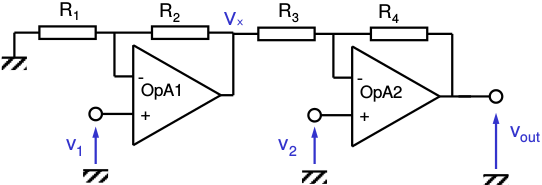
\includegraphics[scale=0.4]{ch4/image2.png}
	\captionof{figure}{ }
	\end{wrapfigure}
	Considérons un exemple "réel". Cette machine est constituée de 
	\begin{itemize}
	\item[$\bullet$] Un inducteur, sur le stator possédant $p$ paires de 
	pôles saillants. La répartition de l'induction dans l'entrefer a une 
	forme trapézoïdale avec comme axe de symétrie l'axe \textit{longitudinal} 
	$d$. L'axe électriquement $\perp$ à celui-ci est l'axe \textit{transversal},
	$q$.
	\item[$\bullet$] 	Un induit, disposés sous la forme d'enroulements de 
	conducteurs placés dans les encoches du cylindre rotorique. On connecte 
	via les faces latérales du cylindre ces conducteurs pour former un 
	\textit{enroulement en tambour.} 
	\end{itemize}\ 
	
	Les conducteurs actifs réunis par ces liaisons sont situés sous les 
	pôles opposés, d’où il résulte une addition des f.e.m. induites.
	Le point médian de chaque conducteur est relié à une lame du collecteur. 
	La \textbf{commutation} d’une lame à l’autre se fait donc au moment 
	où un conducteur actif passe d’un pôle à l’autre. Il faut voir que la somme des 
	f.e.m est nulle dans toute la machine, ce n'est qu'au niveau des ballais où on 
	somme d'une part toutes les f.e.m positives et sur l'autre les négatives. Ces 
	groupes de conducteurs actifs sont appelé \textbf{dérivations}.
	
	
	\subsection{Machine multipolaire}
	\begin{wrapfigure}[8]{l}{4.5cm}
	\vspace{-5mm}
	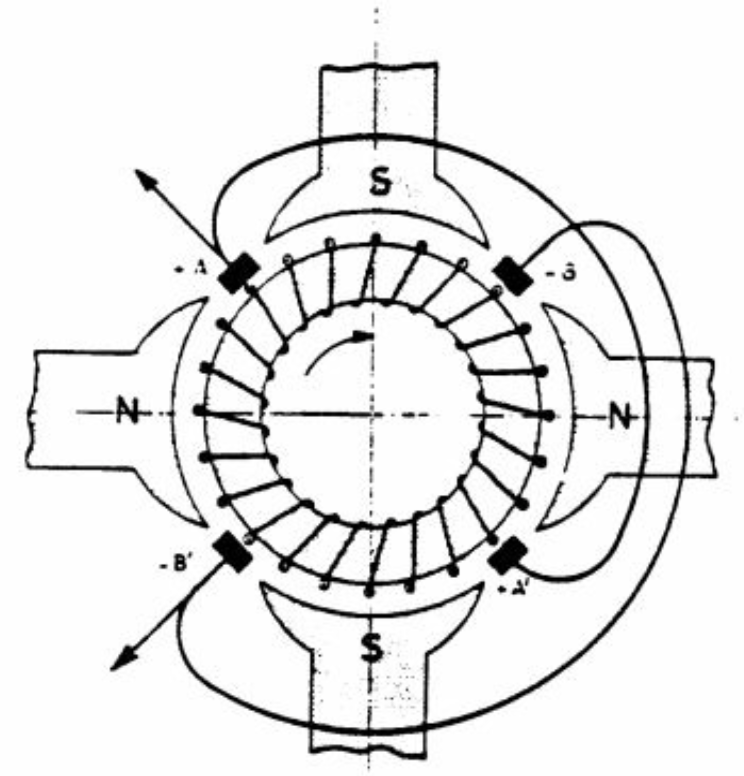
\includegraphics[scale=0.3]{ch4/image2p.png}
	\captionof{figure}{ }
	\end{wrapfigure}
	On considérait jusqu'ici des machines à deux pôles inducteurs, soyons 
	fous et plaçons-en maintenant quatre. Par symétries, les f.e.m. seront 
	égales en grandeurs puisqu'on somme une tension soit positive soit négative 
	entre deux ballais\footnote{Enes se représente la situation du sens des courants en utilisant $q\vec{v}\times \vec{B}$ qui donne des courants entrant aux pôles N et des courants sortant aux pôles S. Sachant que $v = \frac{d\phi}{dt} = \frac{d}{dt}\int \vec{B} \vec{dS}$ et que la convention d'Haelterman disait que le $\vec{dS}$ est donné par la règle de la main droite quand on tourne avec le courant, on peut voir que le produit scalaire de B et dS est positif avant les ballais + et négatif avant les ballais -. C'est comme ça qu'il expliquerai la sélection des ballais positif et négatif.}. Si l'on connecte les balais opposés entre eux (
	les deux négatifs ensemble, de même pour les positifs) on obtient une 
	dynamo multipolaire à \textit{enroulement parallèles}. \\\\\\
	
	\subsection{Types d'enroulement d'induit}
	Problème complexe non abordé ici. Sachez juste que pour l'enroulement 
	en tambour, on peut avoir l'enroulement \textit{imbriqué} ou l'
	enroulement \textit{ondulé}.
	
	\subsection{Tension à vide en régime statique}
	Soit un enroulement en tambour (l'armature, $a$) de $N_C$ conducteurs 
	répartis uniformément en deux couches. Le nombre de spires $N_S=N_C/2$. 
	On va supposer l'induit infiniment divisé de sorte à avoir une densité 
	linéique de spires $N_S/(2\pi R)$. On suppose un rotor lisse.
	
		\subsubsection{Méthode des champs}
		\begin{wrapfigure}[11]{l}{4.8cm}
		\vspace{-5mm}
		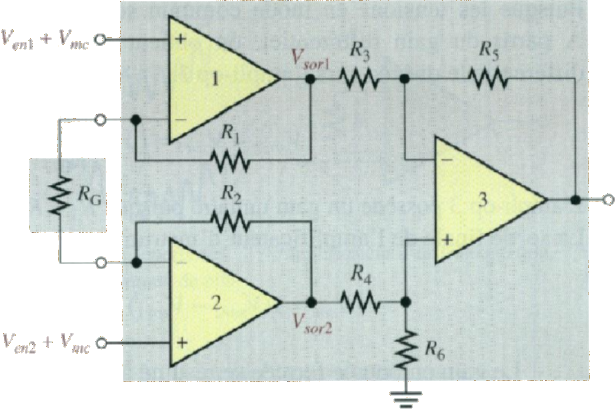
\includegraphics[scale=0.4]{ch4/image3.png}
		\captionof{figure}{ }
		\end{wrapfigure}
		Soit une spire constituée d'un conducteur d'entrée 1 et de sortie 
		1'. Nous avons
		\begin{description}
		\item[$\beta_m$ :] la coordonnée angulaire mécanique de l'entrée 1
		\item[$\beta_m-\alpha_m$ :] la coordonnée mécanique de sortie 1'
		\end{description}				
		La f.e.m. engendrée dans la spire vaut (voir figure ci-contre pour 
		la convention de signe (conducteur entrant et sortant))
		\begin{equation}
		\begin{array}{ll}
		e_{spire} &= B(\beta_m)lv - B(\beta_m-\alpha_m)lv\\
		&= (B(\beta_m)-B(\beta_m-\alpha_m))lv
		\end{array}
		\end{equation}
		Si $\alpha_m = \pi/p$ la spire est \textit{diamétrale}. Le "sens" 
		du champ $B$ sera donc exactement opposé
		\begin{equation}
		\begin{array}{l}
		B(\beta_m-\alpha_m) = - B(\beta_m)\\
		\hookrightarrow e_{spire} = 2B(\beta_m)lv
		\end{array}
		\end{equation}
		Si $\alpha_m<\pi/p$ on parle de spire \textit{à pas raccourci} : 
		on définit 1" déphasé de $\pi/p$ en avant par rapport à 1' et 
		donc déphasé de $\delta_m = \pi/p-\alpha_m$ par rapport à 1. Par 
		symétrie\footnote{??}
		\begin{equation}
		 \begin{array}{ll}
		B(1') = -B(1")\qquad\text{ou}\qquad B(\beta_m-\alpha_m) &=-B(\beta_m
		-\alpha_m+\frac{\pi}{p})\\
		&=-B(\beta_m+\delta_m)		
		\end{array}
		\end{equation}
		Impliquant que $e_{spire} = e_1-e_{1'}=e_1+e_{1"}$, en considérant 
		$B>0$ sous la pôle nord.\\
		On peut alors avoir une répartition rectangulaire de l'induction
		\begin{center}
		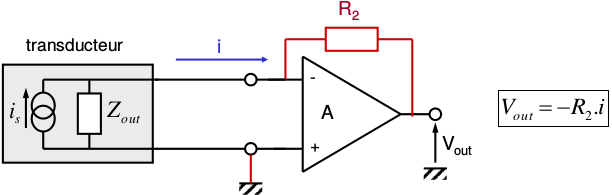
\includegraphics[scale=0.5]{ch4/image4}
		\end{center}
		ou  trapézoïdale 
		\begin{center}
		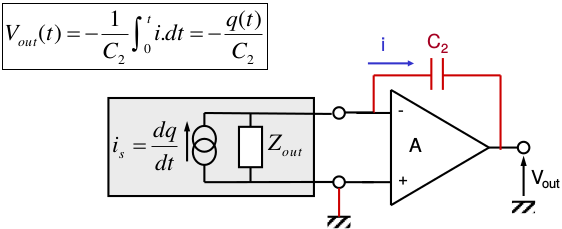
\includegraphics[scale=0.5]{ch4/image5}
		\end{center}
		
		\textsc{Forces électromotrice entre balais}\ \\
		\begin{wrapfigure}[12]{l}{6cm}
		\vspace{-2mm}
		\begin{equation}
		\begin{array}{ll}
		e &= \displaystyle p \int_{-\frac{\pi}{2p}}^{\frac{\pi}{2p}} 
		e_{spire}.\text{densité de spire}\\
		&= \displaystyle p \int_{-\frac{\pi}{2p}}^{\frac{\pi}{2p}} (
		2B(\beta_m)kv)\frac{N_s}{2d\pi}\ d\beta_m\\
		&= \displaystyle \frac{p}{d}N_s\frac{\Omega_r}{\pi} \int_{-
		\frac{\pi}{2p}}^{\frac{\pi}{2p}}B(\beta_m)lR\ d\beta_m\\
		&= \displaystyle\frac{p}{d}N_s\frac{\Omega_r}{\pi}\Phi
		\end{array}
		\end{equation}

		\end{wrapfigure}
		Supposons un enroulement à spires diamétrales tel que $e_{spire} = 
		2B(\beta_m)lv$. La f.e.m. entre balais est constante si l'induit 
		est infiniment divisé. Considérons un enroulement ondulé à $2d$ 
		dérivations : une dérivation comporte $N_S/(2d)$ spires. Celle-ci 
		est constitués par des spires dont les conducteurs d'entrée et 
		de sorties sont sous des pôles de même signe, il y a donc 
		$(N_S/2d).(1/\pi)$ spires appartenant à une dérivation par rad. 
		mécanique. Pour obtenir la tension aux bornes de la dérivation, 
		il faut intégrer les tensions de chaque spire de la dérivation. 
		Comme il y a $p$ paires de pôles, il convient de multiplier le 
		résultat d'un pôle par $p$. De façon générale :\\
		
		\retenir{\begin{equation}
		e = K\ \Omega_r\ \Phi
		\label{eq:4.5}
		\end{equation}
		où	$\Phi$ est le flux utile (coupé par une spire diamétrale 
		d'axe longitudinal de l'induit) par pôle, $\Omega_r$ en rad/s et 
		$K$, une constante qui dépend des données de l'enroulement.}\ \\

		\begin{wrapfigure}[12]{l}{4.8cm}
		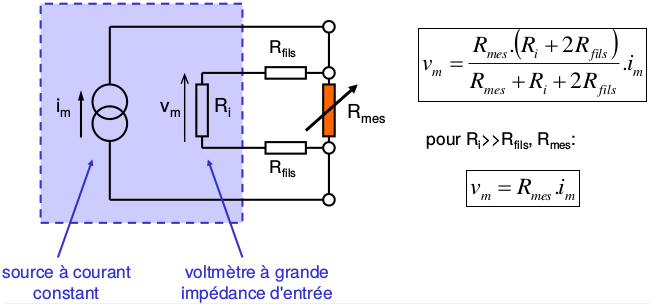
\includegraphics[scale=0.4]{ch4/image6.png}
		\captionof{figure}{ }
		\end{wrapfigure}
		La f.e.m. (tension à vide) d'une dynamo est $\propto$ au flux 
		utile par les pôles et la vitesse de rotation. Cette formule 
		reste valable pour une machine en charge ($i_a\neq0$) si on 
		considère que $\Phi$ pourrait être modifié par $i_a$. $\Phi$ 
		dépend de $i_e$ de façon non-linéaire (cf. labo).\\
		
		Ci-contre, la répartition des f.e.m. engendré pour une dynamo 
		à induit infiniment divisé de spires diamétrales. La tension 
		entre deux balais est la somme ($\int$) de toutes les f.e.m. 
		sous un même pôle. Ce schéma confirme que la f.e.m. est bien 
		alternative mais constante en un point fixe : 
		\textbf{pseudo-stationnaire} du à l'effet redresseur du 
		collecteur.

		\subsubsection{Méthode des circuits}
		\begin{wrapfigure}[10]{r}{2.8cm}
		\vspace{-5mm}
		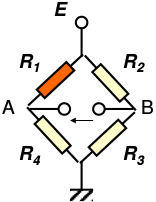
\includegraphics[scale=0.5]{ch4/image7.png}
		\captionof{figure}{ }
		\end{wrapfigure}
		Soit deux enroulements : un d'excitation parcouru par $i_e$ 
		et un induit pseudo-stationnaire à vide. A bornes du balais, 
		on a donc
		\begin{equation}
		v_a = R_ai_a+D\Psi_a
		\end{equation}
		où $\Psi_a$ est le flux coupé par l'enroulement induit, flux 
		créé par le courant d'excitation. On peut écrire
		\begin{equation}
		\Psi_a = M(\beta_m,i_e)i_e
		\end{equation}
		où $M$ est l'inductance mutuelle entre les enroulement $e$ 
		et $a$, mutuelle fonction de $\beta$, l'angle de décalage 
		entre $N$ et l'axe d'enroulement. En faisant les math ;
		\begin{equation}
		\begin{array}{ll}
		(v_a)_{i_a=0} &= \displaystyle D\Psi_a\\
		&= \displaystyle D(Mi_e)\\
		&= \displaystyle  DM\ i_e + M\ Di_e\\
		&= \displaystyle \frac{\partial M}{\partial \beta_m}D\beta_m
		i_e + \frac{\partial M}{\partial i_e}Di_e i_e + M\ Di_e\\
		&= \displaystyle G(\beta_m,i_e)\Sigma_r i_e +\left(M+\frac{
		\partial M}{\partial i_e}i_e\right)Di_e
		\end{array}
		\end{equation}
		On définit alors la valeur locale (ou différentielle) de la 
		mutuelle : $\displaystyle M' = M+\frac{\partial M}{\partial 
		i_e}i_e$, qui sera nulle si les balais sont calés sur l'axe 
		neutre ($\beta = \pi/2$) car $a \perp e$. \\
		On définit également la \textbf{fonction d'excitation}
		\begin{equation}
		G(i_e) = \frac{\partial M(\beta_m,i_e)}{\partial \beta_m}) =
		\frac{(\partial \Psi_a/\partial \beta_m)}{i_e}\qquad si\qquad 
		\beta=\frac{\pi}{2}, i_e=\text{ cste}
		\end{equation}
		La f.e.m. vaut alors $e = (v_a)_{i_a=0} = G(i_e)i_e\Omega_r$ 
		qui ressemble à notre belle formule encadré plus haut ! On 
		peut dès lors écrire
		\begin{equation}
		G(i_e)i_e = K\Phi
		\end{equation}
		La connaissance de la caractéristique à vide qui conduisait 
		immédiatement à la détermination de $K, \Phi$ en fonction de 
		$i_e$, il en est de même pour $G$ en fonction de $i_e$.
		
	\subsection{Effet de décalage des balais}
	\begin{wrapfigure}[7]{r}{9.5cm}
	\vspace{-8mm}
	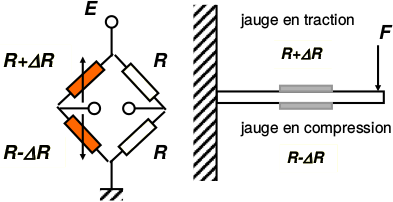
\includegraphics[scale=0.5]{ch4/image8.png}
	\captionof{figure}{ }
	\end{wrapfigure}
	Dans l'expression de la tension à vide, on a maintenant comme 
	limites $-\frac{\pi}{2}p+\gamma_m$ et $\frac{\pi}{2}p+\gamma_m$ (à 
	la place de $-\frac{\pi}{2}p+$ et $\frac{\pi}{2}p$), réduisant la 
	valeur de celle-ci par rapport à leurs positions sur les axes neutres. 
	Il faut encore rajouter à ça un effet de mutuelle.
	
	\subsection{Tension à vide - modèle mathématique}
	Trois remarques sur ce qu'est un bon modèle
	\begin{enumerate}
	\item Adapté au but poursuivi, ça ne sert à rien de faire trop.
	\item Il doit être simple, sinon avoues que tu ne le liras pas.
	\item Il doit être homogène, si on applique une hypothèse il faut 
	toujours l'appliquer.
	\end{enumerate}\ \\
	
	\textsc{Exemple - dynamo à vide}\\
	Définissions comme variables de commande $v_e$ la tension aux bornes 
	du circuit d'excitation, $\Omega_r$ la vitesse de rotation et $e$, 
	la tension à vides aux bornes des balais comme variable de sortie. 
	Connaissant deux expressions pour $e$, il suffit d'en prendre une et 
	de la compléter par l'équation du circuit d'excitation pour obtenir le 
	modèle recherché : $v_e = R_ei_e +D\Psi_e$.
	
		\subsubsection{Modèle non-linéaire}
		Il suffit d'utiliser une relation non-linéaire entre $\Psi_e$ 
		et $i_e$ pour compliquer le tout : $\Psi_e = L_e(i_e)i_e$ où 
		$L_e$ est l'inductance propre du circuit d'excitation, fonction 
		non-linéaire. Si l'on considère que $\Psi_e$ est variable d'état :
		ré-écrivons notre équation sous la forme d'une ED :
		\begin{equation}
		D\Psi_e = v_e-R_ei_e(\Psi_e)
		\end{equation}
		Si cette fois on choisi $i_e$ comme variable d'état, on peut 
		écrire
		\begin{equation}
		\dfrac{\partial \Psi_e}{\partial i_e}Di_e = v_e-R_ei_e\quad 
		\Longrightarrow\quad Di_e = \dfrac{v_e - R_ei_e}{L_e'}
		\end{equation}
		où $L_e'(i_e)$ est la valeur différentielle de l'inductance 
		propre du circuit $e$. Notons qu'elle est aussi égale à 
		$L_e+(\partial L_e/\partial i_e)i_e = \partial\psi_e/\partial 
		i_e$. Sachant que $e = (v_a)_{i_a=0} = G(i_e)i_e\Omega_r$, le 
		calcul de $e$ est immédiat si l'on a $i_e$.\\

		\begin{wrapfigure}[6]{l}{7cm}
		\vspace{-8mm}
		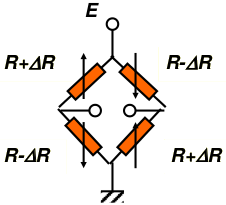
\includegraphics[scale=0.5]{ch4/image9.png}
		\captionof{figure}{ }
		\end{wrapfigure}
		Nos deux équations trop stylées 
		\begin{equation}
		\begin{array}{ll}
		v_e &= R_ei_e + L_e Di_e\\
		e &= K\Phi\Omega_r = G\Omega_ri_e
		\end{array}
		\end{equation}
		nous fournissent un schéma équivalent dont la caractéristique 
		permet le passage de $\Psi_e$ à $i_e$.
		
		Il est également possible, via $D\Psi_e = v_e - R_ei_e(\Psi_e)$ 
		d'obtenir le schéma-bloc suivant :
		\begin{center}
		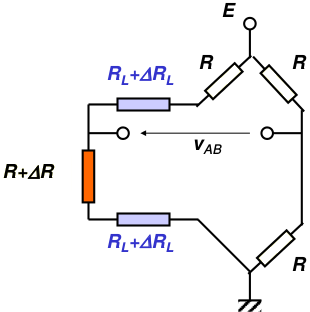
\includegraphics[scale=0.5]{ch4/image10.png}
		\captionof{figure}{ }		
		\end{center}			
		
		\subsubsection{Modèle linéaire}
		On peut l'obtenir en considérant de "petits mouvements" et en 
		substituant les courbes par leurs tangentes. Supposons que 
		$L_e = L_e' = L_{e,ns} = \text{cste}$ et $G = G_{ns} = 
		\text{cste}$. Notre précédente relation devient alors 
		\begin{equation}
		Di_e = \frac{v_e - R_ei_e}{L_e} \quad \lt\quad I_e(p) : 
		\frac{1}{1+pT_e}\frac{V_e(p)}{R_e}
		\end{equation}
		où $T_e = L_e/R_e$ est la constante de temps du circuit d'
		excitation (valeur assez élevée comme beaucoup d'enroulements). 
		Cette relation obtenue via Laplace est assez évidente à vue 
		du schéma équivalent, car ce-dernier est constitué de $R_e$ 
		et $L_e$. La grandeur de sortie vaut toujours 
		\begin{equation}
		e = Gi_e\Omega_r
		\end{equation}
		et dépend linéairement de $i_e$ si la vitesse est constante. 
		Le système global est du premier ordre
		\begin{equation}
		E(p) = G\Omega_r I_e(p) = G\Omega_r \dfrac{1}{1+pT_e}\frac{V_e
		}{R_e}
		\end{equation}
		\begin{center}
		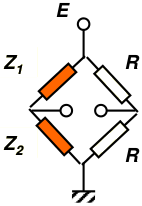
\includegraphics[scale=0.5]{ch4/image11.png}
		\captionof{figure}{ }		
		\end{center}			
		
			
\section{Influence du courant d'armature}
En effet, ça on sent que la machine en charge comportera en plus d'une 
source de tension une résistance $R_a$ et une inductance $L_a$.

	\subsection{Effet Joule (résistance $R_a$)}
	On les trouve dans l'enroulement ainsi que dans le ballais/collecteur,
	dépendant de plusieurs paramètres tel que la température et la valeur du courant.
	Mesurer la résistance globale n'est pas aisé, la résistance n'étant 
	pas la même quand la machine est en fonction ou non : en rotation, 
	elle est perturbée par la f.e.m. rémanente. En gros, les chutes sont 
	\begin{equation}
	\Delta V_{R_a} = \Delta V_b\text{sign}(i_a) + R_ai_a
	\end{equation}
	où $\Delta V_b$ représente la chute balais collecteur (fonction du 
	sens de rotation) et $R_a$ la résistance entre enroulements. Par 
	\textbf{convention}, la chute est fixée à $2V$ pour les balais en 
	carbone et $0.6V$ pour les métalliques.
	
	\subsection{Réaction transversale de l'armature infiniment divisée}
	\begin{wrapfigure}[9]{l}{4.7cm}
	\vspace{-5mm}
	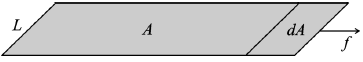
\includegraphics[scale=0.34]{ch4/image12.png}
	\captionof{figure}{ }
	\end{wrapfigure}
	Soit une génératrice avec un courant infiniment divisé qui circule 
	dans l'induit, même sens que la f.e.m. Les courants induits créent 
	à leurs tour un champ créant un flux perpendiculaire au flux 
	inducteur. En désignant $\beta_m$ l'abscisse angulaire d'un point, 
	calculons les ampères-tours dans un contour d'induction fermé :
	\begin{equation}
	\frac{N_c}{2\pi}\frac{i_a}{2d}2\beta_m
	\end{equation}
	Par symétrie par rapport à l'axe des pôles, la moitié des A.t. est 
	attribué à la moitié du chemin. Par abus, on attribue des A.t. la 
	ou le chemin traverse l'entrefer. Si ce dernier est constant et le 
	fer parfait 
	\begin{equation}
	H(\beta_m) = \frac{N_c}{2\pi}\frac{i_a}{2d}\frac{\beta_m}{\delta}
	\end{equation}
	$H$ est max si $\beta_m=\pi/2p$ : 
	\begin{equation}
	H\left(\frac{\pi}{2p}\right) = \frac{N_c}{2\pi}\frac{i_a}{2d}\frac{
	\pi}{2p\delta} = \frac{N_c}{8\delta}\frac{i_a}{pd}=\frac{N_s}{4\delta}
	\frac{i_a}{pd}
	\end{equation}
	Si le fer est réel il suffit de multiplier par $\mu_0$. Tout ceci 
	est bien indépendant de la vitesse de rotation : la situation est 
	la même que si une bobine était alignée sur l'axe neutre.
	
		\begin{center}
		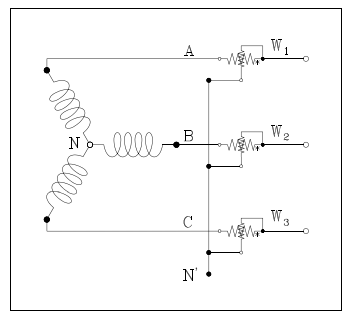
\includegraphics[scale=0.35]{ch4/image13.png}
		\captionof{figure}{ }		
		\end{center}
	
	Pour calculer $L_a$ on considère un enroulement fictif dont toutes 
	les spires ont par axe celui du balai : le flux vaudra l'intégrale 
	de l'induction entre $\beta_m et \pi-\beta_m$. Grâce au flux 
	totalisé : $L_a=\Psi_a/i_a$.
	
	\subsection{Le champ résultant}
		\subsubsection{Sans saturation}
		\begin{wrapfigure}[7]{r}{4.7cm}
	\vspace{-25mm}
	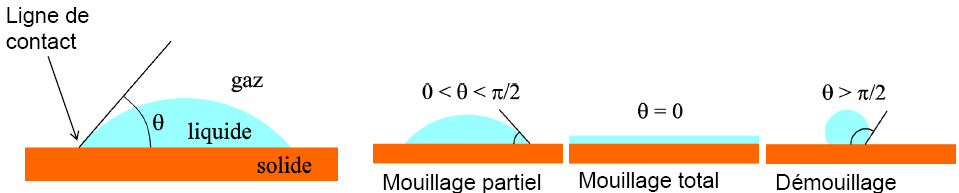
\includegraphics[scale=0.34]{ch4/image14.png}
	\captionof{figure}{ }
	\end{wrapfigure}
		On peut appliquer le principe de superposition. Pour une dynamo, 
		une fois la réaction d'induit est magnétisante (corne d'entrée) 
		et une fois démagnétisant (corde de sortie). La figure ci-contre 
		montre comment obtenir $B$ par la somme de l'induction de l'inducteur 
		$B_e$ et la réaction d'induit $B_a$.\\
		Notons que le flux par pôle n'a pas changé, la f.e.m. en charge est la 
		même qu'à vide. Cependant, l'induction est tantôt plus grande tantôt plus 
		faible par endroit, donc certaines spires supportent plus de tensions et il y a 
		risque de claquage entre les lames du collecteur. 
		
		\subsubsection{Avec saturation}
		L'induction en charge est plus petite que la somme de l'excitation 
		et la réaction d'induit. Le flux longitudinal est plus faible, 
		causant une f.e.m. plus faible $\rightarrow$\textit{ La réaction 
		d'induit possède une composante longitudinale à cause de la 
		saturation.}. Pour décrire l'effet démagnétisant, trois hypothèses :
		\begin{enumerate}
		\item Lignes de forces radiales dans l'entrefer.
		\item L'induction null en dehors des pôles.
		\item Démonstration faite pour $p=d=1$.
		\end{enumerate}
		A vide, juste avec le courant d'excitation $i_e$ on a $A.t._e = 
		N_ei_e$. Si la spire n'est pas sous le pôle sa tension est nulle. 
		Si par contre elle est sous le pôle elle sera $\propto B_e$. La 
		courbe a vide donne le lien entre $e$ et $N_ei_e$ mais aussi la 
		f.e.m. à une constante près.\\
		Les courants induits causent également des A.t. de réactions 
		d'induits qui varient linéairement entre la corne de sortie $-A$ 
		et d'entrée $+A$ de la sorte :
		\begin{equation}
		A = \frac{N_c}{2\pi}\frac{i_a}{2}\frac{b_i}{4\pi R}
		\end{equation}
		Les A.t. varient ainsi linéairement de $N_ei_e-A$ à $N_ei_e+A$ (
		$OP_1$ à $OP_2$ sur le schéma page 4.33). \textbf{Lire le texte 
		sur cette page, c'est assez confus. Enes confirme.}
		
		\subsection{Couple électromécanique - Couple extérieur}
		La loi de Laplace ($F+ilB$) permet de calculer la somme sur 
		chaque conducteur pour ensuite les sommer, mais il est plus 
		simple d'utiliser la conservation de la puissance : la somme 
		de la puissance appliquée électriquement et de la puissance 
		appliquée mécaniquement est nulle\footnote{? (en convention 
		récepteur)} :
		\begin{equation}
		[\underbrace{P_{electrique} - (P_{pJoule}}_{P_{electromecanique}}
		+P_{pmagn})] + [P_{mecan}-P_{meca}]=0
		\end{equation}
		où les pertes joules $P_{pJ}=0$ si $î_a=0$. Par contre les pertes 
		magnétiques existent tout de même (hystérèse, Foucault, ...). Les 
		pertes méca sont dues aux frottement (fonction de $\Omega_r$). La 
		puissance mécanique appliquée à un moteur est négative. On peut 
		calculer le couple électromécanique $P_{em} = C_{em}\Omega_r$. D'autre part,
		\begin{equation}
		\begin{aligned}
			P_{em} &= P_{électrique} - P_{pJ}\\
						 &= v_a i_a - \Delta V_b i_a -R_a i_a^2\\
						 &= e i_a
		\end{aligned}
		\end{equation}
		En utilisant \autoref{eq:4.5}, on trouve que 
		\begin{equation}
			C_{em} = K\Phi i_a = Gi_ei_a.
		\end{equation}
		En moteur, la réaction d'induit change de signe : magnétisante sous la corne polaire d'entrée.\\
		
		\textbf{Réécriture de Nicolas Englebert}
		
	\subsection{Inconvénients de la réaction d'induit}
	Cette réaction cause trois effets néfastes :
	\begin{enumerate}
	\item Déplacement de la ligne neutre ($B=0$) gênant la commutation
	\item Augmente l'indiction : risque de claquage entre les lames
	\item Cause de l'inductance du rotor, s’opposant aux variations rapides 
	du courant induit et donc du couple
	\end{enumerate}
	
	
	\subsection{La commutation}
	La commutation concerne tous les phénomènes inversant le signe du courant 
	par court-circuit/circuit ouvert avec les balais. Comme il y a frottement, 
	il peut y avoir étincelles !
	
	\begin{description}
	\item[Causes mécaniques] Certaines lames bombées, vibrations, mauvais 
	équilibrage, \dots
	\item[Causes électriques] Théoriquement très compliqué
	\end{description}
	Détaillons légèrement ce point \textit{compliqué} avec la théorie de ARNOLD. 
	On se débarasse d'abord de toute imperfections mécaniques en trois hypothèses :
	état mécanique parfait, résistivité balais/collecteur constante, égalité de 
	la largeur d'un balai et d'une lame.\\
	
	Le souci est inductif. Au moment de la commutation, l'inductance à tendance 
	à ne pas laisser passer le courant. Plus mathématiquement, à cet instant la 
	dérivée du courant subit une discontinuité causant une surtension importante : 
	rupture de l’isolation et risque de claquage.\\
	
	Au cours oral, le prof a dit qu'il ne poserait pas de question de démonstration sur cette partie. Lire et comprendre le phénomène au travers les équations peut s'avérer utile. \\
	
	\textsc{Le remède de grand-mère}.\\
	L'idée est de créer un phénomène d'amplitude 
	contraire et même encore plus fort (pour être sûr) pour contrecarrer cet 
	effet. On crée alors une fem opposée, favorable à la variation de courant afin 
	de permettre la variation de courant en fin de commutation. On crée cette fem 
	grâce a un flux d'axe neutre (transversal) au sens opposé à la réaction d'induit. On a dès lors l'intégration de pôles de commutation avec des enroulements de compensation. \\
	On pourrait aussi se dire \textit{"Pourquoi ne pas prendre un entrefer plus grand?"} 
	Effectivement, l'inductance diminue mais le flux d'excitation également ce qui 
	est moins avantageux. 
		

\section{Étude de la dynamique des machines}
	\subsection{Modèles mathématiques - schémas équivalents}
		\begin{wrapfigure}[10]{l}{8.7cm}
	%\vspace{-25mm}
	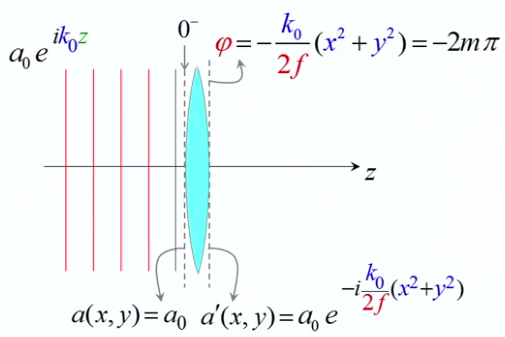
\includegraphics[scale=0.34]{ch4/image15.png}
	\captionof{figure}{ }
	\end{wrapfigure}
	Reprenons ce qui a été vu précédemment et synthétisons le sur le schéma ci-contre. 
	On va supposer que le modèle magnétique, les pertes, \dots sont linéaires. On 
	trouve 
	\begin{description}
	\item[$R_e$;] Résistance du circuit inducteur
	\item[$L_e$;] Inductance du circuit inducteur
	\item[$R_a$;] Résistance du circuit d'induit
	\item[$\Delta V_b$;] Chute de tension du contact balais-collecteur
	\item[$L_a$;] Inductance du circuit d'induit
	\item[$e$;] Force électromotrice engendrée $= Gi_e\Omega_r$
\end{description}		
	Notre tension d'excitation $V_e$ pourra être éventuellement réglable : $V_x$. La 
	zone en pointillé représente la machine, tandis que la partie de droite représente 
	le rotor, possédant une fem $e$ du à sa rotation.\\
	
	Lors de l'allumage, il faut fournir énormément de flux. Pour limiter ce courant, on 
	introduit des réhostas :
	\begin{description}
	\item[$R_d$ : rhéostat de démarrage;]  Sert à limiter le courant à la mise sous tension 
	$V_{al}$ car à vitesse nulle, $e=0$ et le courant est juste limité par $R_a$ et $L_a$ 
	de faible valeur.
	\item[$R_{exc}$ : rhéostat d'excitation;] Règle le courant d'excitation $i_e$ pour une 
	tension d'excitation $v_x$ donnée.
	\end{description}
	Les équations de ce modèles sont, pour rappel :
	\begin{equation}
	\begin{array}{ll}
	v_x &= (R_e+R_{exc}-i_e + L_e\frac{di_e}{dt}\\
	v_{al} &= e+\Delta V_b + (R_a+R_d)i_a + L_a\frac{di_a}{dt}\\
	e &= k\phi\Omega_r = Gi_e\Omega_r
	\end{array}
	\end{equation}
	Cette fois-ci, on doit ajouter l'équation de mouvement :
	\begin{equation}
	j\dfrac{d\Omega_r}{dt} = C_{em}+C_r
	\end{equation}
	avec $C_r$, le couple résistant du moteur (pertes magnétiques et mécanique). 
	Il doit être vu comme négatif, diminuant le couple appliqué par le moteur à l'arbre, 
	$C_{em}$.\\
	Il s'agit d'un modèle dynamique (dérivée). En laboratoire, tout peut être mis comme 
	étant constant. Sous la forme canonique, on obtient :
	\begin{equation}
	\begin{array}{ll}
	Di_e &= \frac{1}{L_e}[v_x-(R_e+R_{exc}i_e]\\
	Di_a &= \frac{1}{L_a}[v_{al} - \Delta V_b - Gi_e\Omega_r - (R_a+R_d)i_a]\\
	D\Omega_r &= \frac{1}{J}[Gi_ei_a - C_r(\Omega_r)]
	\end{array}
	\end{equation}
	Avec ces équations, il est facile d'obtenir le schéma bloc ci-dessous.  
	\begin{itemize}
	\item[$\bullet$] Notre sortie est bien la vitesse de rotation, définie par le couple 
	moteur.
	\item[$\bullet$] La première équation est représenté à gauche sur la branche $V_x$ : 
	on calcule $i_e$ à partir de $V_x$.
	\item[$\bullet$] La grandeur d'entrée de la deuxième équation est la tension d'alimentation. 
	Il faut ainsi partir de $V_{al}$, soustraire $Gi_e\Omega_r,\dots$. Le $Gi_e$ avait déjà été 
	calculé, $\Omega_r$ est à la sortie. Le rectangle central correspond ainsi à une partie de 
	cette deuxième équation
	\item[$\bullet$] Pour la troisième équation, nous avons $K\phi i_a$ et il faut rentrer 
	le couple résistant : on peut dire que le couple résistant dépend de la vitesse de 
	rotation
	\end{itemize}
	
	\begin{center}
	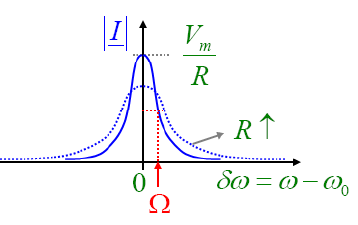
\includegraphics[scale=0.34]{ch4/image21.png}
	\captionof{figure}{ }
	\end{center}
	
	Supprimons la dernière rétroaction. Mettons notre pied sur l'intégrale pour avoir un couple 
	constant. Le couple moteur étant constant, la vitesse ne change pas directement (du à la grande 
	inertie)(nous 
	étions en situation de régime, on vient de briser cet équilibre). Mais maintenant, on sait que 
	la vitesse va diminuer. Sachant cela,  le carré avec (*) au milieu va être affecté. Comme 
	$i_e$ est contant, la fem $e$ va diminuer : déséquilibre le rond avec $\pm$.\\
	
	A l'examen oral, je peux négliger le bras tout en haut en affirmant que c'est un effet 
	correcteur pas très important, que l'ordinateur peut se charger de le calculer.\\
	
	Ceci étant dit, La valeur $V-e$ va commencer à être positive, le courant va alors 
	augmenter. Le couple moteur va alors lui aussi augmenter pour retrouver le couple appliqué 
	par mon pied et on retrouvera un nouveau point d'équilibre, avec une vitesse plus faible 
	mais un courant plus important (car couple plus important).\\
	
	Si la vitesse diminue de 1\%, la vitesse fait-elle de même ? Le courant augmentera en 
	réalité plus rapidement que cette diminution. Pour savoir à quel point, il faut annuler 
	toutes les dérivée pour se rendre compte que le terme $1/R_a$ est très important : le couple 
	va vite réagir à une petite variation.\\
	
	En faisant une analyse semblable, on peut voir que si on augmente $V_x$, le moteur va 
	tourner moins vite. L'augmentation de $V_d$ cause par contre une augmentation de la 
	vitesse.
	
	
\section{Courbes caractéristiques des génératrices}
	
	\subsection{Les différents types de génératrices}
	\begin{wrapfigure}[7]{l}{3cm}
	\vspace{-5mm}
	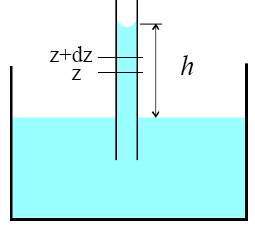
\includegraphics[scale=0.34]{ch4/image16.png}
	\captionof{figure}{ }
	\end{wrapfigure}
	On a toujours considéré que le courant d'excitation était fourni par une source 
	extérieure. Or, à cause du rémanent, une tension existe lors de la rotation entre 
	les balais de la machine pour un courant d'excitation nul. L'idée est d'utiliser 
	ce courant pour exciter la machine\footnote{Oh oui elle est chaude !}.\\
	S'il n'y a pas de charge, $i_e$ est très petit et on considère que la tension aux 
	bornes est la fem. Pour $\Omega_r$ donné, on a deux caractéristiques :
	\begin{enumerate}
	\item Caractéristique à vide $e = f(i_e)$.
	\item Loi d'Ohm du circuit d’excitation $e=(R_{exc}+R_e)i_e$.\footnote{En régime, 
	il n'y a que les résistances : la self se comporte comme un fil.}
	\end{enumerate}
	\begin{center}
	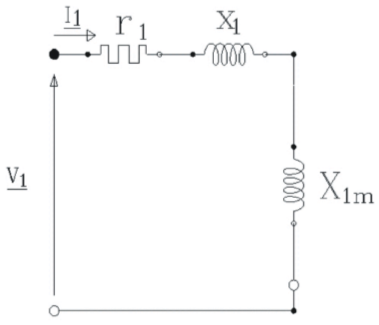
\includegraphics[scale=0.37]{ch4/image17.png}
	\captionof{figure}{ }
	\end{center}
	L'intersection donne le point de fonctionnement. On voit qu'il existe une valeur 
	de $R_{exc}$ au dela de laquelle la tension aux bornes est très faible (a). Si 
	on inverse les bornes, la machine ne s'amorce pas et si la machine est linéaire, 
	le seul point de fonctionnement est $e=0,i_e=0$ sauf si $R_{exc}+R_e=G\Omega_r$.\\
	
	En pratique, on rencontre trois types de génératrices :
	\begin{description}
	\item[Excitation dirigée / shunt] Beaucoup de spires pour avoir beaucoup 
	d'ampères-tours avec peu de flux
	\item[Excitation série] Ce type de moteur est caractérisé par le fait que 
	le stator (inducteur) est raccordé en série avec le rotor (induit) : le même 
	courant traverse le rotor et le stator. Cela offre une faible résistance, et 
	le nombre de spire nécessaire est moins important ($\approx 100$ fois moins qu'en 
	shunt).\footnote{ On fait tourner le moteur : entre les balais on obtient $e$. Pour avoir 
	le flux, on passe tout le courant dans l'excitation.}
	\item[Compoundage] Les deux en même temps.
	\end{description}
	
	
	\subsection{Caractéristiques à vide et en charge d'une machine à excitation 
	indépendante}
		\subsubsection{Fem à vide}
			\begin{wrapfigure}[7]{r}{3.3cm}
	\vspace{-5mm}
	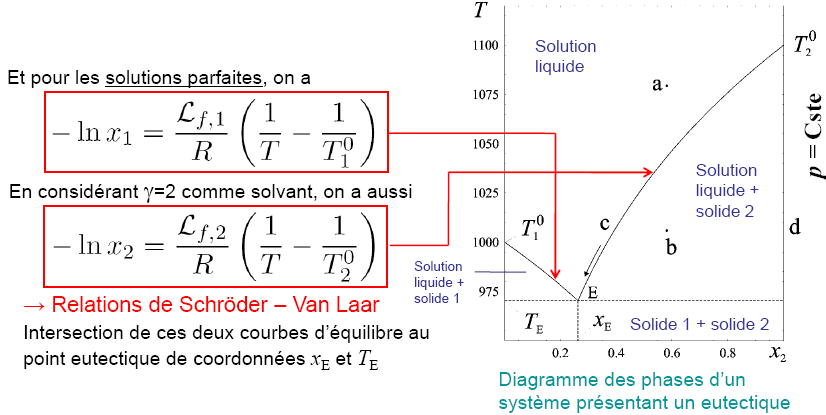
\includegraphics[scale=0.34]{ch4/image18.png}
	\captionof{figure}{ }
	\end{wrapfigure}
		Négligeons l'hystérèse. Ici on place le voltmètre sur les balais pour mesurer 
		la fem à vide. Le courant $i_e$ comprend le rhéostat et le rémanent n'est 
		pas représenter. Initialement la courbe est "droite" puis on arrive à saturation.
		
		
		\subsubsection{Fem et tension en charge}
		La tension aux bornes de la machine est donnée par (courant de charge fixé) :
		\begin{equation}
		v_a = e - R_ai_a - \Delta V_b
		\end{equation}
		où $e$ vaut la fem à vide correspondant à $i_e' = i_e-i_{eri}$ où $i_{eri}$ 
		est le courant d’excitation correspondant aux A.t. démagnétisant de la réaction 
		d'induit.\\
		\danger Si le flux est perpendiculaire, cela n'influe pas sur d'autres flux.\\

		\begin{center}
		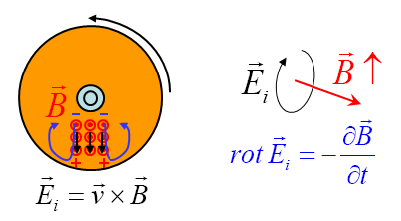
\includegraphics[scale=0.43]{ch4/image19.png}
		\captionof{figure}{ }
		\end{center}		
		
		\begin{wrapfigure}[9]{l}{3.3cm}
		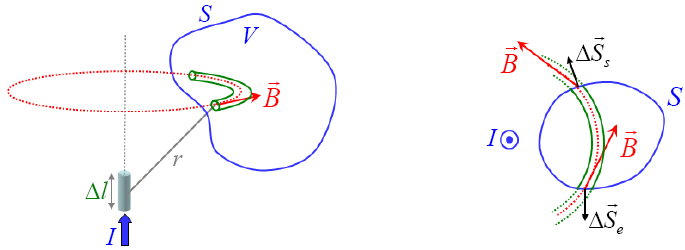
\includegraphics[scale=0.34]{ch4/image20.png}
		\captionof{figure}{ }
		\end{wrapfigure}
		On déduit le caractéristique en charge de celle à vide en décalant chaque 
		point du triangle des pertes $ABC$ où $AB$ vaut $i_{eri}$ et $BC$ vaut 
		$R_ai_a + \Delta V_b$. En supposant que pour $i_a$ fixé, $R_a/i_{eri} =\ cste$, 
		on déduit la caractéristique en charge par translation $AC$.\\
				
		En pratique, $i_{eri} =\ cste$ si $i_a =\ cste$ n'est vérifiée que pour un 
		petit domaine, les courbes ne sont pas des parfaites translation. On remarque 
		sur la courbe réelle, qu'au début, il n'y a pas de réaction d'induit. Ces 
		courbes sont également commune "à la fin" à cause de la saturation.
		
		
\section{Courbes caractéristiques des moteurs}
On cherche à caractériser le courant consommé par le moteur, $i_a$ et $-C$ le couple 
net appliqué à la charge tel que
\begin{equation}
-C = C_{em} - C_{pmeca} - C_{pmagn}
\end{equation}
		
	\subsection{Caractéristique à vide en moteur $\Omega_r = f(i_e)$}
	Supposons $V_{al}$ constante, $R_d=0$ (en régime), $R_a$ constante (pas d'effet 
	thermique) et négligeons $\Delta V_b$. On suppose que la caractéristique à vide,
	en génératrice, 	prise à la vitesse de référence $\Omega_g$ est connue :
	\begin{equation}
	e_{0g} = f(i_e)
	\end{equation}
	Mais aussi la famille des courbe des f.e.m. en charge :
	\begin{equation}
	e_g = f(i_e,i_a)\qquad \forall i_a
	\end{equation}
	La caractéristique à vide du moteur lie $\Omega_r = f(i_e)$ pour $V_a=\ cste$ et 
	couple moteur nul. Le couple EM sert alors juste à compenser les pertes mécaniques : 
	courant absorbé très faible\footnote{Car le moteur n'entraîne rien}, tension aux 
	bornes $\approx$ fem à vide :
	\begin{equation}
	v_a = e+R_ai_a + \Delta V_B \approx e \approx e_0
	\end{equation}
	On on sait que (en moteur) $\displaystyle e_0 = K\Phi(i_e)\Omega_r \Longrightarrow 
	\Omega_r = 	\dfrac{e_0}{K\Phi(i_e)}$. Pour la même valeur du courant d’excitation, 
	la caractéristique à vide (en génératrice) donne $e_{0g} = K\Phi(i_e)\Omega_g$. On a donc :
	\begin{equation}
	\Omega_r = 	\dfrac{e_0}{K\Phi(i_e)}\ \ \text{ feat. }\ \ \left\{\begin{array}{ll}
	v_a &\approx e_0\\
	\frac{1}{K\Phi(i_e)} &= \frac{\Omega_g}{e_{0g}(i_e)}
	\end{array}\right.\quad  \Longrightarrow\quad \Omega_r = \Omega_g\dfrac{v_a}{e_{0g}(i_e)}
	\end{equation}
	
	\begin{wrapfigure}[9]{l}{5.3cm}
	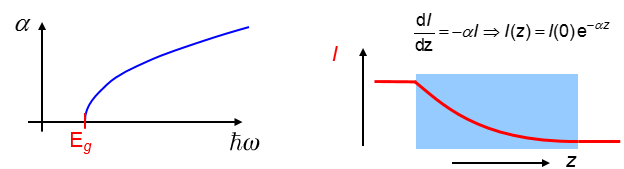
\includegraphics[scale=0.34]{ch4/image22.png}
	\captionof{figure}{ }
	\end{wrapfigure}
	On remarque que la caractéristique à vide en moteur est, à une constante près, 
	l'inverse de celle en génératrice. On voit que la vitesse \textbf{diminue} quand 
	$i_e$ \textbf{augmente}\footnote{Comme vu précédemment sur le schéma bloc à cause 
	de la rétroaction!} Il faut démarrer le moteur à pleine excitation ($i_e=i_{max}$) 
	pour avoir le couple moteur maximal. On voit également que si on diminue trop 
	l'excitation (coupe un fil) la vitesse augmente : danger mécanique $\rightarrow$ le 
	courant n'est plus limité que par la résistance d'induit et peut atteindre dix 
	fois le courant nominal. Les disjoncteurs se chargent de protéger la machine.
	
	
	\subsection{Caractéristiques en charge - moteur à excitation indépendante}
	On peut voir le "en charge" comme un freinage, charge dont le couple résistif est 
	connu. La puissance mécanique va changer et il y aura des effets sur la vitesse et 
	la consommation (le courant d'alimentation change même si la tension d'alimentation 
	est constante).\\
	On suppose que $i_e=\ cste$ et $v_a =\ cste = V_{al}$. On sait que :\\
	
	\retenir{\begin{equation}
	\begin{array}{ll}
	v_a &= e+ \Delta V_b + R_ai_a\\
	e &= K\Phi\Omega_r\\
	C_{em} &= K\Phi i_a\\
	-C &= C_{em} - C_p\\
	e_g &= f(i_e,i_a)\quad \text{à $\Omega_g$ donné)}\\
	K\Phi &= \frac{e}{\Omega_r} = \frac{e_g}{\Omega_g}
	\end{array}
	\end{equation}
	avec $C_p$ le couple des pertes (frottement, Foucault, \dots). L'ensemble des 
	courbes mesurées en génératrice est donnée par $e_g$. Comme le flux est difficile 
	à mesurer, 	on le calculera via $e_g/\Omega_g$ avec $\Delta V_b$ négligé (dernière 
	équation). Notons qu'il n'y a ici pas de dérivée : nous sommes en régime.}\ 
	
	Nous avons donc
	\begin{equation}
	\begin{array}{ll}
	\Omega_r &= \dfrac{e}{K\Phi}\\
	&= \dfrac{v_a -\Delta V_b\text{sign}(i_a) - R_ai_a}{e_g/\Omega_g}\\
	&= \Omega_g\dfrac{v_a -\Delta V_b - R_ai_a}{e_g}	
	\end{array}
	\end{equation}
	
		\subsubsection{a. $\Omega_r = f(i_a)$}
		Supposons la réaction d'induit négligeable : $e_g(i_e,i_a) = e_{0g}(i_e)$. D'où
		\begin{equation}
		\Omega_r = \Omega_g \dfrac{v_a-\Delta V_b\text{ sign}(i_a)}{e_{0g}(i_e)}- 
		\Omega_g \dfrac{R_ai_a}{e_{0g}(i_e)}
		\end{equation}

\begin{center}
	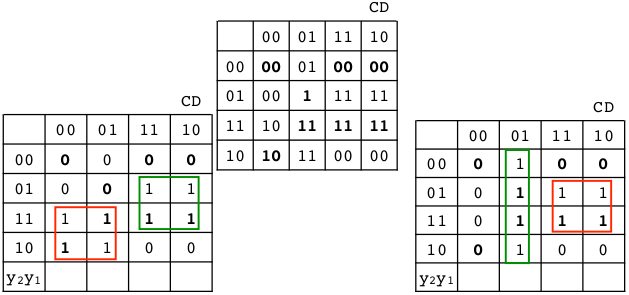
\includegraphics[scale=0.34]{ch4/image23.png}
	\captionof{figure}{ }
\end{center}
		Comme $R_a$ est très petit, notre terme sera presque une droite horizontale : à 
		$V_a, i_e=\ cste$, la vitesse de rotation à excitation indépendante dépend peu de 
		la charge. C'est rassurant, car nous avions vu que la vitesse n'allait que peu 
		changer quand on dépose son pied ! Le 	"saut" à l'intersection avec l'ordonnée 
		correspond à la variation de signe au niveau des balais. \\
		Quand on augmente $i_e$, $e_{0g}$ augmente aussi\footnote{Nos fameuses courbes $e_0$ 
		en fonction de $i_e$ (sans tenir compte de $i_a$ ici.} et la vitesse à vide diminue : 
		déplacement caractéristique (idem si $V_a$ diminue). \\
		
		Avec une réaction d'induit, pour $i_e$ fixé, la fem en charge $e_g$ diminue quand 
		$i_a$ augmente : augmentation de la vitesse de rotation en moteur aux valeurs 
		élevée du courant.
		\begin{center}
			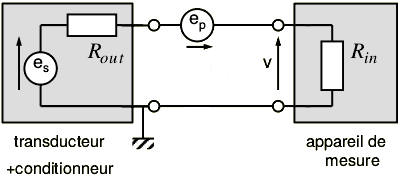
\includegraphics[scale=0.5]{ch4/image24.png}
	\captionof{figure}{Pour l'oral, ceci est un bon complément au schéma bloc vu plut haut! 
	Donne une explication plus matheuse.}
		\end{center}
	
		\subsubsection{b. $-C = f(i_a)$}
		Dans ce cas-ci on a : 
		\begin{equation}
		C_{em} = K\Phi i_a = \dfrac{g(i_e,i_a)}{\Omega_g}i_a
		\end{equation}
		avec $-C = C_{em}-C_p$. Attention, $C_{em}$ n'est pas le couple mécanique net utile ! 
		Pour $e_g(i_e,i_a)$ on utilise la courbe en génératrice et $\Omega_g$ est constante 
		en génératrice. \\
		Si la réaction d'induit est négligeable avec $i_e$ constant et $e_g=e_{0g}$ constant, 
		$C_{em}$ est linéaire en fonction du courant absorbé $i_a$. Comme la vitesse ne varie 
		que peu, il en est de même pour le couple de perte : le couple moteur est aussi linéaire 
		en fonction de $i_a$.
	

	
	
	
	
	
	
	
	
	
	
	
	
	
	
	
	
	
	
	
	
	
	
	
	
	
	
	
	
	
	
	
	
	
		
		

 %%%%%%%%%%%%%%%
%	Ch5 : Boundary layer	 %
%%%%%%%%%%%%%%%

\chapter{Boundary layer}

\section{Derivation of the boundary layer equations}
	\begin{wrapfigure}[10]{l}{5cm}
	\vspace{-5mm}
	\includegraphics[scale=0.23]{ch5/1}
	\captionof{figure}{}	
	\end{wrapfigure}
	Let's remind that in the introduction we analysed the circumstances in whihch viscous forces can be neglected and the conclusion was that it was caracterized by the Reynold's number. When it is large, it means that viscous forces are small compared to convective inertial forces. Despite the small order of magnitude of viscous forces, they can't be neglected everywhere (walls). This leads us to consider 2 region around a body : 
	\ \\
	\begin{itemize}
		\item[•] \textbf{the distal or outer zone}: wherer the flow is inviscid so viscous forces are negligible (ch3). 
		\item[•] \textbf{the thin, proximal or inner zone}: where viscous stresses may not be neglected, leading to the boundary \textbf{layer} $\mathbf{\delta}$ which is next to a solid wall and a region behind the body called the \textbf{wake} (sillage). \\
	\end{itemize}
	
	We hope that, similarly to the inviscid case where equations simplifies, the case will be here because of the small thickness of the boundary layer. We make a first assumption saying that if $C$ is the caracteristic length of the body in the tengential direction and $\delta$ the one in the normal direction

	\begin{equation}
		when \ Re_C \gg 1 \qquad \Rightarrow \delta \ll C
	\end{equation}
	The whole chapter is based on constant density flows, so the governing equation in 2D are
	
	\begin{equation}
	\begin{aligned}
		&\frac{\D u_1}{\D x_1} + \frac{D u_2}{\D x_2} = 0\\
		&\rho \left[ u_1 \frac{\D u_1}{\D x_1} + u_2 \frac{\D u_1}{\D x_2} \right] = -\frac{\D p}{\D x_1} + \mu \left( \frac{\D ^2 u_1}{\D x_1^2} + \frac{\D ^2 u_1}{\D x_2^2} \right) \\
		&\rho \left[ u_1 \frac{\D u_2}{\D x_1} + u_2 \frac{\D u_2}{\D x_2} \right] = -\frac{\D p}{\D x_2} + \mu \left( \frac{\D ^2 u_2}{\D x_1^2} + \frac{\D ^2 u_2}{\D x_2^2} \right)
	\end{aligned}
	\end{equation}
	
	These equations are for a coordinate system established to study the outer flow. Now as we analyse the flow in a fin layer close to the body it is convinient to rewrite the flow equations in a body fitted curvilinear system where $x$ is the curvilinear coordinate tengent to the body and $y$ the one normal to the body. If we can assume that $\delta \ll R$ which is the body radius of curvature (variable), the transformed curvilinear equations are identical to the original cartesian equations
	
	\begin{equation}
		\begin{aligned}
		&\frac{\D u}{\D x} + \frac{\D v}{\D y} = 0\\
		&\rho \left[ u \frac{\D u}{\D x} + v \frac{\D u}{\D y} \right] = -\frac{\D p}{\D x} + \mu \left( \frac{\D ^2 u}{\D x^2} + \frac{\D ^2 u}{\D y^2} \right) \\
		&\rho \left[ u \frac{\D v}{\D x} + v \frac{\D v}{\D y} \right] = -\frac{\D p}{\D y} + \mu \left( \frac{\D ^2 v}{\D x^2} + \frac{\D ^2 v}{\D y^2} \right)
	\end{aligned}
	\end{equation}
	
	The condition $\delta \ll R$ is the most likely to be violated where R is the smalest, which corresponds to the front of the body. But let's imagine that the condition is fullfilled. In these equations we didin't use $\delta$ so let's rewrite these equations in non-dimensional form by choosing the non-dimensional variables $(\tilde{x}, \tilde{y}, \tilde{u}, \tilde{v}, \tilde{p})$ in such a way that they'll be of order of magnitude 1
	
	\begin{equation}
	\begin{aligned}
		&\tilde{x} = \frac{x}{C} \qquad\qquad  \tilde{u} = \frac{u}{\uinf} \qquad\qquad  \tilde{p} = \frac{C_p}{2} = \frac{p-p_0}{\rho\uinf ^2}\\
		&\tilde{y} = \frac{y}{\delta} \qquad \qquad \ \tilde{v} = \frac{v}{v_\delta (?)} 
	\end{aligned}
	\end{equation}
	
	where for $u$ we know that for the inviscid case we considered $\uinf$ as velocity of the flow on the body and $v$ was null on the body wall so we have a "?". The continuity equation in dimensionless variables will help us 
	
	\begin{equation}
		\frac{\uinf}{C}\frac{\D \tilde{u}}{\D \tilde{x}} + \frac{v_\delta}{\delta}\frac{\D \tilde{v}}{\D \tilde{y}} = 0 \qquad \Rightarrow \underbrace{\frac{\D \tilde{v}}{\D \tilde{y}}}_{\theta (1)} = - \frac{\uinf}{C} \frac{\delta}{v_\delta} \underbrace{\frac{\D \tilde{u}}{\D \tilde{x}}}_{\theta (1)} \qquad \Rightarrow \frac{\uinf}{C} \frac{\delta}{v_\delta} = \theta (1) \Leftrightarrow v_\delta = \theta \left( \frac{\delta \uinf}{C}\right)
	\end{equation}	 
	
	where $\theta (1)$ means order of magnitude 1. We are going to replace $v_\delta = \frac{\delta \uinf}{C}$. We are going to do the same operation for momentum equations. Let's begin with the tengential momentum equation
	
	\begin{equation}
	\begin{aligned}
		&\rho \left[ \frac{\uinf ^2}{C}\tilde{u} \frac{\D \tilde{u}}{\D \tilde{x}} + \frac{\uinf ^2 \cancel{\delta}}{C} \frac{\tilde{v}}{\cancel{\delta}}\frac{\D \tilde{u}}{\D \tilde{y}} \right] = -\rho \frac{\uinf ^2}{C} \frac{\D \tilde{p}}{\D \tilde{x}} + \mu \left( \frac{\uinf}{C^2}\frac{\D ^2 \tilde{u}}{\D \tilde{x}^2} + \frac{\uinf}{\delta ^2}\frac{\D ^2 \tilde{u}}{\D \tilde{y}^2} \right) \\
		\Leftrightarrow \qquad &\rho \frac{\uinf ^2}{C}\left[ \tilde{u} \frac{\D \tilde{u}}{\D \tilde{x}} +  \tilde{v} \frac{\D \tilde{u}}{\D \tilde{y}} + \frac{\D \tilde{p}}{\D \tilde{x}}  \right] =  \mu \frac{\uinf}{\delta ^2} \left( \cancel{\frac{\delta ^2}{C^2}\frac{\D ^2 \tilde{u}}{\D \tilde{x}^2}}+ \frac{\D ^2 \tilde{u}}{\D \tilde{y}^2} \right) \\
	\end{aligned}
	\end{equation}
	
	where we make appear $\frac{\delta ^2}{C^2}$ which is much smaller than one if $Re_C \gg 1$. Because of all the dimensionless variables are of order of magnitude 1 $\theta (1)$ the two constants must be of the same order of magnitude
	
	\begin{equation}
		C\frac{\rho \uinf ^{\cancel{2}}}{C^2} \frac{\delta ^2}{\mu \cancel{\uinf}} = \theta (1) \qquad \Leftrightarrow \left( \frac{\delta}{C}\right)^2 = \theta \left( \frac{\mu}{\rho \uinf C}\frac{1}{Re _C} \right) =  \qquad \Rightarrow \delta = \theta \left(\frac{C}{\sqrt{Re_C}} \right) \ll C
	\end{equation}
	
	which confirms the assumption $\delta \ll C$ when $Re_C\gg 1$. From now we will take $\delta = \frac{C}{\sqrt{Re_C}}$. To conclude, it remains the normal momentum equation 
	
	\begin{equation}
	\begin{aligned}
		&\rho \left[ \frac{\uinf ^2 \delta}{C^2}\tilde{u} \frac{\D \tilde{v}}{\D \tilde{x}} + \frac{\uinf ^2 \delta^{\cancel{2}}}{C^2} \frac{\tilde{v}}{\cancel{\delta}}\frac{\D \tilde{v}}{\D \tilde{y}} \right] = -\rho \frac{\uinf ^2}{\delta} \frac{\D \tilde{p}}{\D \tilde{y}} + \mu \left( \frac{\uinf \delta}{C^3}\frac{\D ^2 \tilde{v}}{\D \tilde{x}^2} + \frac{\uinf\delta}{C\delta ^{2}}\frac{\D ^2 \tilde{v}}{\D \tilde{y}^2} \right) \\
		\Leftrightarrow\qquad &\rho \frac{\uinf ^2\delta}{C^2}\left[ \tilde{u} \frac{\D \tilde{v}}{\D \tilde{x}} +  \tilde{v} \frac{\D \tilde{v}}{\D \tilde{y}}  \right] = - \rho\frac{\uinf ^2}{\delta} \frac{\D \tilde{p}}{\D \tilde{y}} +  \mu \frac{\uinf }{C\delta} \left( \cancel{\frac{\delta ^2}{C^2}\frac{\D ^2 \tilde{v}}{\D \tilde{x}^2}}+ \frac{\D ^2 \tilde{v}}{\D \tilde{y}^2} \right) \\
		\Leftrightarrow\qquad  &\rho \uinf ^2\left[ \tilde{u} \frac{\D \tilde{v}}{\D \tilde{x}} +  \tilde{v} \frac{\D \tilde{v}}{\D \tilde{y}}  \right] = - \rho\uinf^2\left(\frac{C}{\delta}\right) ^2 \frac{\D \tilde{p}}{\D \tilde{y}} +  \mu\uinf \underbrace{\left(\frac{C}{\delta}\right)^2}_{Re_C = \rho\frac{C\uinf}{\mu}} \frac{1}{C} \frac{\D ^2 \tilde{v}}{\D \tilde{y}^2}\\
		\Leftrightarrow\qquad  &\rho \uinf ^2\left[ \tilde{u} \frac{\D \tilde{v}}{\D \tilde{x}} +  \tilde{v} \frac{\D \tilde{v}}{\D \tilde{y}}  \right] = - \rho\uinf^2\left(\frac{C}{\delta}\right) ^2 \frac{\D \tilde{p}}{\D \tilde{y}} +  \frac{\cancel{\mu}\uinf}{\cancel{C}} \rho\frac{\cancel{C}\uinf}{\cancel{\mu}} \frac{\D ^2 \tilde{v}}{\D \tilde{y}^2}\\
				\Leftrightarrow\qquad  &\underbrace{\tilde{u} \frac{\D \tilde{v}}{\D \tilde{x}} +  \tilde{v} \frac{\D \tilde{v}}{\D \tilde{y}} -  \frac{\D ^2 \tilde{v}}{\D \tilde{y}^2}}_{\theta (1)} = - \left(\frac{C}{\delta}\right) ^2 \frac{\D \tilde{p}}{\D \tilde{y}} \qquad \Rightarrow \frac{\D \tilde{p}}{\D \tilde{y}} = \theta \left(\frac{\delta}{C}\right) ^2 
	\end{aligned}
	\end{equation}

	where we see that the pressure gradient accross the boundary layer normal to the wall cannot be of order of magnitude 1 but of that of $\left(\frac{\delta}{C}\right) ^2$ which is \textbf{negligible}

	\begin{equation}
		\tilde{p}(\tilde{x}, \tilde{y}) = \tilde{p}_e (\tilde{x}) \qquad \Rightarrow p(x,y) = p_e(x) 
	\end{equation}

	where $p_e(x)$ is the outer inviscid flow pressure distribution. The pressure variation inside the boundary layer beeing null, the pressure inside is equal to the outer pressure distribution computed on the wall. The pression is no longer an unknown. The final form of the equations in the boundary layer are 

	\begin{equation}
	\begin{array}{l|l}
		\frac{\D \tilde{u}}{\D \tilde{x}} + \frac{\D \tilde{v}}{\D \tilde{y}} = 0	 & 	\quad\frac{\D u}{\D x} + \frac{\D v}{\D y} = 0\\
	 		\tilde{u} \frac{\D \tilde{u}}{\D \tilde{x}} +  \tilde{v} \frac{\D \tilde{u}}{\D \tilde{y}} = -\frac{d \tilde{p}_e}{d \tilde{x}}	+ \frac{\D ^2 \tilde{u}^2}{\D \tilde{y}^2}\quad & 	\quad	 \rho \left[ u \frac{\D u}{\D x} + v \frac{\D u}{\D y} \right] = -\frac{d p_e}{d x} + \mu \frac{\D ^2 u}{\D y^2}\\
	 		\tilde{p}(\tilde{x}, \tilde{y}) = \tilde{p}_e (\tilde{x}) 	&\quad p(x,y) = p_e(x) 
	\end{array}
	\end{equation}
	
	So it means that if we replace the third equation in the second, we end up with a system of two equations and two unknowns. We also see that the geometry of the body does not appear at all in the equations since we assumed that $\delta \ll R$. The boundary layer is only sensitive the pressure distribution.
	

\section{Zero-pressure gradient (flat plate) boundary layer}
	\begin{wrapfigure}[6]{l}{6cm}
	\vspace{0mm}
	\includegraphics[scale=0.23]{ch5/2}
	\captionof{figure}{}	
	\end{wrapfigure}
	We want to solve the simpliest problem using this when there is no pressure gradient. This correspond to a uniform flow over a flat plate of 0 thickness. The coordinate system is the cartesian one and the outer flow is the uniform flow because the flat plate does not perturb the flow. So for the inviscid flow 
	
	\begin{equation}
		u = \uinf \qquad v = 0 \qquad p = p_\infty \qquad \Rightarrow p_e(x) = p_\infty \Rightarrow \frac{dp_e}{dx} = 0
	\end{equation}
	
	\newpage
	The simplified equations and the initial condition IC and boundary conditions BC are
	
	\begin{equation}
	\begin{aligned}
		&\frac{\D u}{\D x} + \frac{\D v}{\D y} = 0\\
		&u \frac{\D u}{\D x} + v \frac{\D u}{\D y} = \nu \frac{\D ^2 u}{\D y^2}
	\end{aligned}	
	\qquad
	\begin{aligned}
	&IC: u(0,y) = \uinf\\
	&BC: u(x,0) = v(x,0) = 0 \mbox{ (non-slip)}
	\end{aligned}
	\end{equation}
	
	Then we have also the matching boundary conditions that says to the edge of the boundary layer, the velocity should tend to its inviscid value
	
	\begin{equation}
		\lim _{y\rightarrow \infty} u(x,y) = u_e(x) = u^{inv}(x,0) = \uinf 
	\end{equation}
	the far field limit of the boundary flow should be equal to the inner limit of the outer inviscid flow. So the solution at $\infty$ of the boundary flow should be equal to the solution at 0 of the inviscid flow. This is the matching condition for the tengential velocity and not the normal velocity. We are looking solutions $u(x,y)$ and $v(x,y)$. We'll try to represent the sollution to have an idea of how to find it, for $u(x,y)$ in a 3 dimentional coordinate system $x, y, u$. Following IC, when $x=0$, $u = \uinf$ and $y = 0, u=0$. We see that there is a jump, a discontinuity when $x=0=y$ (\autoref{fig:5.3}).\\
	
	 Another way to represent is to plot $y$ in function of $u$ for various axis (positions x). We already know that $u = \uinf$ in the far field and it start from 0 for all axis. If we look at our boundary profile, we know that $\delta$ is increasing with x, meaning that velocity will vary slower along $y$ for increasing $x$ leading to \autoref{fig:5.4}. These last curves have the same shape, such that we can maybe contract them on a same curve. 
	 
		 \begin{center}
		 \begin{minipage}{0.28\textwidth}
	 		\begin{center}
	 		\includegraphics[scale=0.24]{ch5/3}
	 		\captionof{figure}{}
	 		\end{center}
	 		\label{fig:5.3}
	 \end{minipage}
	 	 \begin{minipage}{0.4\textwidth}
			 \begin{center}
			 \includegraphics[scale=0.24]{ch5/4} 
			 \captionof{figure}{}
			 \end{center}
	 		\label{fig:5.4}
	 \end{minipage}
	 	 \begin{minipage}{0.3\textwidth}
	 	 	\begin{center}
	 	 	\includegraphics[scale=0.235]{ch5/5}
	 		 \captionof{figure}{}
	 	 	\end{center}
	 		\label{fig:5.5}
	 \end{minipage}
		 \end{center}


	 Let's take a value $\uinf /2$ with the half velocity thickness $l_{1/2}(x)$. If we repllot $u/\uinf$ in function of $y/l_{1/2}(x)$, we know that at $\uinf /2$ we will have 1 and 0 at 0. If we assume that all the curves have the same shape, they all pass from these 2 points as represented on \autoref{fig:5.5}. This is called the \textbf{self similarity assumption} and we'll have to check it.  		 \\
		 
	\begin{wrapfigure}[8]{l}{5cm}
	\vspace{-5mm}
	\includegraphics[scale=0.23]{ch5/6}
	\captionof{figure}{}	
	\label{fig:5.6}
	\end{wrapfigure}
	In order to verify the assumption, let's first represents \autoref{fig:5.4} as \autoref{fig:5.6}, this is equivalent to plot the \textbf{contour lines}. The contour $u=\uinf$ is vertical and $u=0$ horizontale, $u=\uinf /2$ will have the equation $y = l_{1/2}(x)$ by definition. If \autoref{fig:5.5} is valid, we will have for example for $\frac{u}{\uinf} = 0.1$, $\frac{y}{l_{1/2}(x)} = c_{0.1}$. So the contour line $u = 0.1 \uinf$ has as equation $y = c_{0.1}l_{1/2}(x)$. We see that in fact the self similarity assumption implies that the contour lines are stretched expression of the same function. 
	
	\newpage
	
	\subsubsection{Coordinate transformation}
		Let's imagine that we make a change of variables 

		\begin{equation}
			\xi = x \qquad \eta = \frac{y}{l_{1/2}(x)} = \frac{y}{l(x)}.
			\label{eq:5.14}
		\end{equation}
		By the way, we use the value at $1/2$ but we could take what we want, the only change is the constant. Now if we plot $\eta$ in function of $\xi$, the self similarity assumption in the case of contour plot means that if all velocity profile have the same value of $x$ so the same $\xi$. It means that the contour lines will be horizontal lines in the transformed variables. So if the transformation induces no variation along $\xi$
		
		\begin{equation}
			u(x,y) \rightarrow u(\cancel{\xi} , \eta ) \qquad \Rightarrow \frac{u}{\uinf} = g(\eta).
		\end{equation}
		
		The solution only depends on $\eta$. This is an assumption and we have to check. For that we have to make the change of variables in the equations using the relation 
		
		\begin{equation}
		\begin{aligned}
		&\forall \varphi (x,y) = \hat{\varphi}(\xi (x,y), \eta (x,y)) \\
			\frac{\partial \varphi}{\partial x} = \frac{\partial \hat{\varphi}}{\partial \xi} 	\frac{\partial \xi}{\partial x} &+ \frac{\partial \hat{\varphi}}{\partial \eta} \frac{\partial \eta}{\partial x} \qquad and \qquad
			\frac{\partial \varphi}{\partial y} = \frac{\partial \hat{\varphi}}{\partial \xi} \cancel{\frac{\partial \xi}{\partial y}} + \frac{\partial \hat{\varphi}}{\partial \eta} \frac{\partial \eta}{\partial y}.
		\end{aligned}
		\end{equation}
		
		We can now compute the derivative of the velocities
		
		\begin{equation}
		\begin{aligned}
			&\frac{\D u}{\D x} = \cancel{\frac{\D (\uinf g)}{\D xi}} \frac{\D xi}{\D x} + \underbrace{\frac{\D (\uinf g)}{\D \eta}}_{\uinf g'} \underbrace{\frac{\D \eta}{\D x}}_{-\frac{y}{l^2(x)}\frac{dl}{dx}} = - \uinf g'(\eta)\frac{y}{l^2(x)}\frac{dl(x)}{dx} = - \uinf g'(\eta)\eta \frac{1}{l(\xi)} \frac{dl(\xi)}{d\xi}\\
			&\frac{\D u}{\D y} = \frac{\D \uinf g}{\D \eta} \frac{1}{l(\xi)} = \uinf \frac{g'}{l(\xi)} \qquad and \qquad \frac{\D ^2 u}{\D y }= \uinf \frac{g''}{l^2(\xi)}
		\end{aligned}
		\label{eq:5.17}
		\end{equation}
		
		\subsubsection{Continuity equation}
			Let's integrate and replace by what we expressed ($\zeta = z/l(\xi), z \equiv y, \zeta \equiv \eta$)
	
			\begin{equation}
			\begin{aligned}
				\frac{\D v}{\D y} =- \frac{\D u}{\D x} = \uinf g'(\eta) \frac{\eta}{l(\xi)} \frac{dl(\xi)}{d\xi} \qquad \Leftrightarrow &v(x,y) - v(x,0) = \uinf \int _0 ^y g'(\zeta) \frac{\zeta}{l(\xi)} \frac{dl(\xi)}{d\xi} \, dz\\
				\Leftrightarrow &v(x,y) = \uinf \frac{dl(\xi)}{d\xi} \underbrace{\int _0 ^\eta g'(\zeta) \zeta  \, d\zeta}_{F(\eta)}
			\end{aligned}	
			\end{equation}
			where if we integrate by part we find $F(\eta) = \eta g - \int g\, d\zeta = \eta f' - f(\eta)$. This implies that \eqref{eq:5.17} becomes 
			
			\begin{equation}
				\frac{\D u }{\D x} = - \uinf f''\eta \frac{1}{l(\xi)} \frac{dl}{d\xi} \qquad \frac{\D u}{\D y} = \uinf \frac{f''}{l} \qquad \frac{\D ^2 u}{\D y }= \uinf \frac{f'''}{l^2}.
			\end{equation}
			
			A first conclusion is that the same similarity of the tengential velocity profile implies a same similarity of the normal velocity profile in the form
			
			\begin{center}
			\theor{
			\begin{equation}
				v = \uinf \frac{dl}{d\xi}(\eta f' - f). 
				\label{eq:5.20}
			\end{equation}
			}
			\end{center}
			
		\subsubsection{Momentum equation}
			We know that $u = \uinf g = \uinf f'$, so the continuity equation becomes
			
			\begin{equation}
			\begin{aligned}
				&\underbrace{\uinf f' \left(  - \uinf f''\eta \frac{1}{l(\xi)} \frac{dl}{d\xi} \right)} + \uinf \frac{dl}{d\xi}(\underbrace{\eta f'} - f) \uinf \frac{f''}{l} = \nu \uinf \frac{f'''}{l^2} \\
				\Leftrightarrow  &- \uinf ^2 \frac{dl}{ld \xi} ff''' = \frac{  \nu \uinf f''}{l^2} \qquad \Leftrightarrow - \uinf ^{\cancel{2}} \frac{dl}{\cancel{l}d \xi} ff'' \frac{l^{\cancel{2}}}{\nu \cancel{\uinf}} = f'''\\
				\Leftrightarrow &-\frac{\uinf l}{\nu} \frac{dl}{d\xi} ff'' = f'''
			\end{aligned}
			\end{equation}
			
			At this stage, we can already conclude something about the validity of the self similarity assumption. Indeed, $l$ is function of $\xi$, $f$ a function of $\theta$, if we bring all $f$ to the right member, we have an equality between a function of $\xi$ and a function of $\eta$. The only way for these to be equal, and so for the assumption to hold, is for the expression to be a \textbf{constant}
			
			\begin{center}
			\theor{
			\begin{equation}
				\frac{\uinf l}{\nu}\frac{dl}{d\xi} = cst \qquad f''' + ff'' = 0
				\label{eq:5.22}
			\end{equation}
			}
			\end{center}
			
			The $l$ is chosen arbitrary so we can choose the constant as wish. We take $cst = 1$. Notice that we can write the last equation in terms of $Re$ as 
			
			\begin{equation}
				Re_l \frac{dl \frac{\uinf}{\nu}}{d\xi \frac{\uinf}{\nu}} = Re_l \frac{dRe_l}{dRe_\xi} = 1 \qquad \Leftrightarrow Re_l^2 = 2 Re_\xi + \cancel{Re_{l_0}^2}.
				\label{eq:5.23}
			\end{equation}
			
			We can easely solve \eqref{eq:5.22}
			
			\begin{equation}
				\frac{\uinf}{\nu}\frac{\frac{dl^2}{2}}{d\xi} = 1 \qquad \Leftrightarrow l^2 = \frac{2\nu}{\uinf} \xi + \cancel{l_0^2} \qquad \Leftrightarrow l = \frac{\sqrt{2}x}{\sqrt{Re_x}}
			\end{equation}
			
			The caracteristic length scale $l_0$ appearing in the equations is the one when $\xi = x = 0$ at the leading edge where $l = 0$. The condition for the self similarity assumption to hold is that the caracteristic length scale is of this form. We have checked the compatibility with the governing equations, we now have to check the IC and BC. 
			
		\subsubsection{Compatibility with IC/BC}
			We have for the initial condition that
			
			\begin{equation}
				IC: \quad u(0,y) = u\inf \qquad \Leftrightarrow \frac{u(0,y)}{\uinf} = g\left(\eta = \frac{y}{l(0)}\right)=1
			\end{equation}
			
			If $l(0)$ was a bounded number, since $y$ can take all values, $\eta$ has an infinite set of value which is impossible. In order to get one value, $l(0) = 0$ or $l(0) = \infty$. The only possible value is $l(0) = l_0 = 0$ which is matching with our result before and we get the condition 
			
			\begin{equation}
				\lim _{\eta \rightarrow \infty} g(\eta) = 1.
			\end{equation}
			
			Now for the boundary condition we have 
			
			\begin{equation}
			BC: 	\quad		
			\begin{aligned}
				&u(x,0) = 0 \qquad \Rightarrow \frac{u(x,0)}{\uinf} = g\left(\eta =\frac{0}{l(x)}\right) = 0 \qquad \Rightarrow f'(0) = 0\\
				&v(x,0) = 0 \qquad \Rightarrow f(0) = 0 \quad \mbox{using } \eqref{eq:5.20}
			\end{aligned}
			\end{equation}
			
			It stays only the matching condition that says 
			
			\begin{equation}
				\lim _{y \rightarrow \infty} u(x,y) = \uinf \qquad \Leftrightarrow \lim _{y \rightarrow \infty} \frac{u(x,y)}{\uinf} = \lim _{\eta \rightarrow \infty} g\left( \eta = \frac{y}{l(x)}\right) = 1
			\end{equation}
			
			\begin{wrapfigure}[9]{l}{5cm}
			\vspace{-5mm}
			\includegraphics[scale=0.23]{ch5/7}
			\captionof{figure}{}	
			\label{fig:5.7}
			\end{wrapfigure}
			We fall on the same condition as the IC. This is fortunate because \eqref{eq:5.22} is a third order equation so it needs only 3 conditions. It remains to find $f$ by solving this equations with these conditions and that's what Blasius did. It looks simple but there isn't analytical solutions, he used expansion in series. The solutions are shown at the top on \autoref{fig:5.7} and at the bottom we find the experimental data giving the velocity profile for various value of $x$. We see that the data nicely collapse with the same curve. But why we determined the boundary layer? For friction! So let's exploite the results.
			
		\subsubsection{Exploitation of the results} 
			Let's remind the expression for friction 
			
			\begin{equation}
				\tau_w = \mu \left( \frac{\partial u}{\partial y}\right)_w  = \frac{\mu}{l} f''(0) \uinf = \sqrt{\frac{\uinf}{2\nu x}}\mu f''(0)\uinf
			\end{equation}
			
			In fluid mecanics we love dimensionless numbers so we use the \textbf{friction coefficient}
			
			\begin{equation}
				C_f = \frac{\tau _w}{\rho \uinf ^2 /2} = \frac{2 \uinf}{\rho \uinf ^2}\sqrt{\frac{\uinf}{2\nu x}} \mu f''(0) = \sqrt{\frac{2\nu}{\uinf x}} f''(0) = \frac{\sqrt{2}f''(0)}{\sqrt{Re_x}} = \frac{2 f''(0)}{Re_l}
			\end{equation}
			
			where the last equivalence comes from \eqref{eq:5.23}. Looking at the table, we find the last result 
			
			\begin{equation}
				C_f = \frac{0.664}{\sqrt{Re_x}}
			\end{equation}
			
			What's the physical interpretation of $l$.  We said it was some percentage velocity thickness. When $\eta = 1$, $f'(\eta) = 0.46$, so $l$ is the $46\%$ velocity $\Rightarrow u = 0.46 \uinf$. Now we want to construct more physically based boundary layer thicknesses. 
			
		\subsubsection{Other characteristic thicknesses}
			\paragraph{Conventional thickness} There is one called the \textbf{conventional thickness} $\delta$ or $\delta _{.99}$, beeing the thickness where velocity reaches 99\% of the outer velocity. So 
			\begin{equation}
				\eta _{\delta} =\frac{\delta _{.99}}{l(x)} \mbox{ is such that } f'(\eta _\delta) = 0.99. 
			\end{equation}
			
			Using the tables we find that it corresponds to 
			
			\begin{equation}
			\begin{aligned}
				&\eta _\delta = 3.5 \qquad \Rightarrow \delta _{.99} = 3.5 l(x) = 3.5 \sqrt{\frac{2\nu x}{\uinf}} \approx 5 \sqrt{\frac{\nu x}{\uinf}} \qquad \Leftrightarrow \frac{\delta _{.99}}{x} = \frac{5}{\sqrt{Re_x}}\\
				&\Rightarrow Re_\delta = 5 Re_x
			\end{aligned}			
			\end{equation}
			
			\begin{wrapfigure}[9]{l}{4cm}
			\vspace{0mm}
			\includegraphics[scale=0.23]{ch5/8}
			\captionof{figure}{}	
			\label{fig:5.8}
			\end{wrapfigure}
			This is necessary because if we take the table and try to identify $\delta _{.99}$, the angle is not accurate. This is no more physical than the 46\% thickness. 
			
			\paragraph{Mass flow defect thickness} Something more physical is found when we replot $\rho u$ in function of $y$ and compare it to the inviscid vertical profile $u = \uinf$. When we integrate the mass flow near the wall, there is a mass flow defecit and a thickness based on which are
			
			\begin{equation}
			\begin{array}{c}
				\mbox{Mass flow deficit} = \rho \int _0 ^\infty (\uinf - u)\, dy \\
				\mbox{Mass flow defect thickness}:\\
				 \delta ^* = \frac{\rho \int _0 ^\infty (\uinf - u) dy }{\rho \uinf} = \int _0 ^\infty \left( 1-\frac{u}{\uinf} \right)\, dy
			\end{array}
			\end{equation}
			
			The value for the flate plate/zero pressure gradient is 
			
			\begin{equation}
				\delta ^* = \int _0^\infty (1- f') l\, dy = l\underbrace{\int _0^\infty (1-f') \, dy}_{\eta ^*}\qquad \Rightarrow Re_{\delta ^*} = Re_{l}\eta ^* = \sqrt{2Re_x}\eta ^* .
			\end{equation}
			
			\begin{wrapfigure}[6]{r}{6.5cm}
			\vspace{-5mm}
			\includegraphics[scale=0.23]{ch5/9}
			\captionof{figure}{}	
			\label{fig:5.9}
			\end{wrapfigure}
			Let's now give a physical meaning to that mass flow deficit. Let's consider the infinitely thick flat plate and a streamline in the outer region flow which is deviated because of the presence of the boundary layer $y(x) \neq y_0$. Mass conservation tells us that 
			
			\begin{equation}
			\begin{aligned}
				&\rho \int _0^{y_0} u_\infty \, dy =  \rho \int _0^y u(x,y) \, dy \qquad \Leftrightarrow \rho \int _0^{y} u_\infty \, dy - \rho \int _{y_0}^{y} u_\infty \, dy = \rho \int _0^y u(x,y)\infty \, dy \\
				\Leftrightarrow \ &\rho \int _0^{y} (u_\infty - u) \, dy = \rho \int _{y_0}^{y} u_\infty \, dy \qquad \Leftrightarrow y-y_0 = \int _0^{y} \left(1 -\frac{u}{\uinf}\right)\, dy = \delta ^*
			\end{aligned}
			\end{equation}
			
			We see that the deviation of the streamline is exactly $\delta ^*$ called the \textbf{displacement thickness}. One last thing to draw attention, we saw that $f'  \rightarrow 1 \Rightarrow f = \eta + C$. This constant is 
			
			\begin{equation}
				C = \lim _{\eta \rightarrow \infty}  (f-\eta ) = \lim _{\eta \rightarrow \infty}  \int _0 ^\eta (f'-1) \, d\eta = \int _0^\infty (f'-1)\, d\eta = -\eta ^*.
			\end{equation}
			
			We can see this on the table graph where if we extrapolate to the x axis we find $\eta ^*$. We have imposed the matching condition to the tengential velocity profile. What's the asymptotic value of the normal velocity? It is the limiting value of $F = \eta f' - f$ 
			
			\begin{equation}
				\lim _{y \rightarrow \infty} v = \uinf \frac{dl}{dx}\eta ^*\neq 0.
			\end{equation}
			
			There we have normal velocity mismatch. This is due to the consideration we made at the beginning saying that streamlines were straight but now we conclude that they are not straight. We do not take into account the perturbation of the outer inviscid flow induced by the presence of the viscous layer. 
			
			\begin{wrapfigure}[11]{l}{4cm}
			\vspace{0mm}
			\includegraphics[scale=0.23]{ch5/10}
			\captionof{figure}{}	
			\label{fig:5.10}
			\end{wrapfigure}
			\paragraph{Momentum flow defect thickness}
			Similarly to the mass flow defect, we can define the momentum flow defect as beeing 
			
			\begin{equation}
				\mbox{MoFD} = \int_0^\infty \rho \left(  \uinf ^2 - u^2 \right) \, dy
			\end{equation}
		
			If we draw attention to to the math definition of the previous $\delta ^*$, we notice that it is the hight in the plot of the rectangle that have the same area as the one formed by the curve. We can define a momentum induced by the mass flow by multiplying its expression by $\uinf$ and by defining the \textbf{extra momentum flow defect} and the corresponding \textbf{momentum flow defect thickness}
			
			\begin{equation}
			\begin{aligned}
				&\mbox{XMoFD} =  \int_0^\infty \rho \left(  \uinf ^2 - u^2 \right) \, dy - \uinf \int_0^\infty \rho \left( \uinf -u \right)\, dy 
= \int_0^\infty \rho u \left(\uinf - u\right) \,  dy\\
				&\mbox{MoFDT} = \frac{\mbox{XMoFD}}{\rho \uinf ^2} = \theta = \int_0^\infty \frac{ u}{\uinf} \left( 1 - \frac{u}{\uinf} \right)\, dy
			\end{aligned}
			\end{equation}
			
			For the case of the flat plate, we know $\frac{u}{\uinf} = f'$, so
			
			\begin{equation}
				\theta = l \underbrace{\int _0^\infty f' (1-f') \, d\eta}_{\theta ^*} = l\theta ^* = \frac{\sqrt{2}x}{\sqrt{Re_x}} \theta ^*.
			\end{equation}
			
			To find the value of $\theta ^*$, we can integrate by part we find
			
			\begin{equation}
			\begin{aligned}
				\theta ^* &= \int _0^\infty (1-f') \underbrace{f' \, d\eta}_{df} = \underbrace{\left[ f (1-f') \right]_0^\infty}_{=0} + \int_0^\infty f f'' \ d\eta\\
				\eqref{eq:5.22} \Rightarrow &= \int_0^\infty - f''' \, dy = f''(0) = 0.664.
			\end{aligned}
			\end{equation}
			
			This conclues this section but keep in mind that we have a normal velocity mismatch. However, in \eqref{eq:5.20} appears $\frac{fl}{dx}$ which is equal by \eqref{eq:5.22} to 
			
			\begin{equation}
				\frac{dl}{dx} = \frac{1}{Re_l}\qquad =0 \ for \ Re_l \rightarrow \infty
			\end{equation}
			
			So we see that the mismatch disappear for Re number going to $\infty$. This means that classical boundary theory is valid only in the case of infinite Re number, for a finite Re there is a finite mismatch. 
			
			
\section{Other pressure gradient}
	The equations and initial conditions are the same except for the pressure term
	
	\begin{equation}
		\begin{aligned}
		&\frac{\D u}{\D x} + \frac{\D v}{\D y} = 0\\
		&u \frac{\D u}{\D x} + v \frac{\D u}{\D y} =- \frac{1}{\rho} \frac{dp_e}{dx}+ \nu \frac{\D ^2 u}{\D y^2}
	\end{aligned}	
	\label{eq:5.44}
	\end{equation}
	
	Because of the variation of the tangential pressure, there is a variation of the tangential velocity. Indeed, if we take the momentum equation for the inviscid flow we have 
	
	\begin{equation}
		u \frac{\D u}{\D x} =- \frac{1}{\rho} \frac{dp_e}{dx}
	\end{equation}
	
	which means that the outer velocity is not constant if the outer pressure is not constant. In other words, for a position $x_1$ we will have a $u_{e_1}$ different of the velocity $u_{e_2}$ of a position $x_2$. We also see that a positive pressure gradient corresponds to a decelarating flow due to the minus sign and vice-versa. We can now wonder if there is also a self-similar solution. 
	
	\begin{center}
	\begin{minipage}{0.49\textwidth}
\begin{center}
	\includegraphics[scale=0.25]{ch5/11}
	\captionof{figure}{}
\end{center}
	\label{fig:5.11}
	\end{minipage}
	\begin{minipage}{0.49\textwidth}
\begin{center}
	\includegraphics[scale=0.25]{ch5/12}	
	\captionof{figure}{}
\end{center}
	\label{fig:5.12}
	\end{minipage}
	\end{center}
	
	If we replot y in funtion of u, we will have a different plot compared to the flat plate because of the changing value of $u_{e_x}$ as shown on \autoref{fig:5.11}. So to make these velocity profiles collapse in a single one we need to scale the velocity and y and not only y as previously. So if we plot $\frac{y}{l(x)}$ in function of $\frac{u}{u_e(x)}$, we must have a single velocity profile with an asymptote at 1, whatever the value of x as shown on \autoref{fig:5.12}. Again we don't know we will have to check. There is a difference between the two plot axis, $l(x)$ is unknown but $u_e(x)$ is known by the calculation on the outer flow. For the same coordinate transformation \eqref{eq:5.14}
	
	\begin{equation}
		\frac{u}{u_e(x)} = g(\cancel{\xi}, \eta)  \qquad \Leftrightarrow u = u_e(x)
	\end{equation}
	
	That's the \textbf{self-similarity assumption}. \eqref{eq:5.17} is therefore valid to the condition of replacing $\uinf$ by $u_e(x)$
	
	\begin{equation}
		\begin{aligned}
			&\frac{\D u}{\D x} = \frac{du_e}{dx}g(\eta ) + u_e\underbrace{\frac{\D g}{\D \eta}}_{u_e(x) g'} \underbrace{\frac{\D \eta}{\D x}}_{-\frac{y}{l^2(x)}\frac{dl}{dx}} = \frac{du_e}{dx}g(\eta )  - u_e(x) g'(\eta)\eta \frac{1}{l(\xi)} \frac{dl(\xi)}{d\xi}\\
			&\frac{\D u}{\D y} = u_e(x)\frac{\D  g}{\D \eta} \frac{1}{l(\xi)} = u_e(x) \frac{g'}{l(\xi)} \qquad and \qquad \frac{\D ^2 u}{\D y }= u_e(x) \frac{g''}{l^2(\xi)}
		\end{aligned}
		\end{equation}
		
		\subsubsection{Continuity equation}
			The process is exactly the same as last time except that we will have the additional term due to $\frac{\D u}{\D x}$ 
			
			\begin{equation}
			\begin{aligned}
				&\frac{\D v}{\D y} = -\frac{\D u}{\D x} = -\frac{du_e}{dx}g(\eta )  + u_e g'\frac{\eta}{l} \frac{dl}{d\xi} \\
				&v(x,y) = -\frac{du_e}{dx} l \int _0 ^\eta \underbrace{g(\zeta) \, d\zeta }_{f}+ u_e \frac{dl}{d\xi} \underbrace{\int _0 ^\eta \zeta g'(\zeta) \, d\zeta}_{F= \eta f' -f} \\
				&v = -l \frac{du_e}{dx} f + u_e \frac{dl}{dx} (\eta f' - f)
			\end{aligned}
			\end{equation}
			
			which is the same expression with an additional term. 
			
		\subsubsection{Momentum equation}
			Knowing that $u = u_e f'$, the momentum equation becomes
				
			\begin{equation}
			\begin{aligned}
				&u_ef' \left[ \frac{du_e}{dx}f' \cancel{- u_e f''\frac{\eta}{l}\frac{dl}{dx}} \right] + \left[-l \frac{du_e}{dx} f + u_e \frac{dl}{dx} (\cancel{\eta f'} - f)\right] u_e \frac{f''}{l} = u_e\frac{du_e}{dx} + \nu u_e \frac{f'''}{l^2}\\
				\Leftrightarrow \qquad &\underbrace{\frac{\nu u_e }{l^2}}_{F_1(x)}f''' + \underbrace{u_e \frac{du_e}{dx}}_{F_2(x)} \left[1 - {f'}^2 + ff'' \right] + \underbrace{ \frac{u_e^2}{l}\frac{dl}{dx}}_{F_3(x)}ff'' = 0 \\
				\Leftrightarrow \qquad &\frac{F_1(x)}{F_3(x)}f''' + \frac{F_2(x)}{F_3(x)}(1-f'^2+ff'') + ff''=0 
			\end{aligned}
			\label{eq:5.49}
			\end{equation}
			
			For this last equation to admit a solution, it must be reductible to a simple function of $\eta$. This implies that \textbf{the self similarity conditions} are
			
			\begin{equation}
				\frac{F_1(x)}{F_3(x)} = cst  =\frac{F_3(x)}{F_1(x)} \qquad and \qquad \frac{F_2(x)}{F_3(x)} = cst = \frac{F_3(x)}{F_2(x)}
			\end{equation}
			
			Let's write completely $\frac{F_2(x)}{F_3(x)}$ and $\frac{F_3(x)}{F_1(x)}$
			
			\begin{equation}
			\begin{aligned}
				&\frac{F_2(x)}{F_3(x)} =  \frac{\frac{du_e}{u_e dx}}{\frac{dl}{ldx}} = \frac{\frac{d\ln u_e}{dx}}{\frac{d \ln l}{dx}} = k \qquad \Leftrightarrow \ln u_e =k \ln l + c \qquad \Leftrightarrow u_e = K l ^k\\
				&\frac{F_3(x)}{F_1(x)} = u_e\frac{dl}{dx} \frac{l}{\nu } = \frac{K}{\nu}l^{k+1}\frac{dl}{dx} = \frac{K}{\nu (k+2)} \frac{dl^{k+2}}{dx} = cst \qquad \Leftrightarrow \left\{\begin{aligned} l &\propto x^{\frac{1}{k+2}}\\
				u_e &\propto x^{\frac{k}{k+2}} \end{aligned}\right.
			\end{aligned}
			\end{equation}
			
			The conclusion is that we will have a solution if the velocity distribution is a power of x 
			
			\begin{center}
			\theor{			
			\begin{equation}
				u_e = ax^m \qquad and \qquad \frac{du_e}{dx} = amx^{m-1} = m\frac{u_e}{x}
			\end{equation}
			}
			\end{center}
			
			Now we can look at $\frac{F_2(x)}{F_1(x)}$ to see what happens
			
			\begin{equation}
				\frac{F_2(x)}{F_1(x)} = \frac{u_e \frac{du_e}{dx}}{\frac{\nu u_e}{l^2}} = cst \qquad \Leftrightarrow l^2 \propto \frac{1}{\frac{du_e}{dx}} \propto \frac{x}{u_e} \qquad \Leftrightarrow l \propto \sqrt{\frac{bx}{u_e}}
			\end{equation}
			
			where $b$ is an arbitrary constant to specify that $l$ is defined up to an arbitrary constant. Let's now compute the coefficients $F_1, F_2, F_3$ 
			
			\begin{equation}
				\frac{\nu u_e }{l^2} = \frac{\nu u_e^2}{bx} \qquad u_e \frac{du_e}{dx} = m\frac{u_e^2}{x} \qquad \frac{u_e^2}{l}\frac{dl}{dx} = u_e^2\frac{d\ln l}{dx} = \frac{u^2}{2} \left( \frac{1}{x} - \frac{m}{x} \right)
			\end{equation}
			
			After simplifying $\frac{u_e^2}{x}$ and replacing in \eqref{eq:5.49}, we have 
			\begin{equation}
				\frac{\nu}{b} f''' + m \left[1 - f'^2 + ff'' \right] + \frac{1}{2} ( 1 - m ) ff'' = 0 = f''' + ff'' \underbrace{\frac{1+m}{2} \frac{b}{\nu}} - f'^2 + \frac{mb}{\nu} (1-f'^2) 
			\end{equation}
			
			$b$ being an arbitrary constant, we will choose it such that we obtain the equation in the case of the flat plate with $\frac{1+m}{2} \frac{b}{\nu} = 1$ which is the 
			
			\begin{center}
			\theor{
			\textbf{Falkner-skan equation}
			\begin{equation}
				b = \frac{2\nu}{1+m} \qquad \Rightarrow f''' + ff'' + \underbrace{\frac{2m}{1+m}}_{\beta} (1-f'^2) = 0
			\end{equation}
			}
			\end{center}
			
			At this stage, let's notice that when: 
			\begin{itemize}
				\item[•] $m>0$: accelerating flow $\Rightarrow \beta > 0$.
				\item[•] $m<0$: decelerating flow $\Rightarrow \beta < 0$.
			\end{itemize}
			
			where $\beta$ can be seen as an acceleration parameter. We can see it easely by seeing that 
			
			\begin{equation}
				\frac{du_e}{dx} = m\frac{u_e}{x} \qquad \Rightarrow l^2 \frac{du_e}{dx} = m \frac{bx}{u_e}\frac{u_e}{x} = \frac{2 m\nu}{1+m} = \beta \nu \qquad \Rightarrow \beta = \frac{l^2}{\nu} \frac{du_e}{dx}
			\end{equation}
			
			where $\beta$ is really related to the velocity gradient. So when the velocity profile is a power of $x$, the self similar solution exist and its shape depends on $\beta$. 
			
\begin{center}
	\begin{minipage}{0.49\textwidth}
\begin{center}
	\includegraphics[scale=0.20]{ch5/13}
	\captionof{figure}{}
\end{center}
	\label{fig:5.13}
	\end{minipage}
	\begin{minipage}{0.49\textwidth}
\begin{center}
	\includegraphics[scale=0.34]{ch5/14}	
	\captionof{figure}{}
\end{center}
	\label{fig:5.14}
	\end{minipage}
	\end{center}
	
			\autoref{fig:5.13} represents these profiles in function of $\beta$. $\beta = 0$ is the zero pressure gradient. For increasing $\beta$ the boundary layer gets stiller and the profile fuller. When $\beta$ decelerate, the boundary layer gets thickker and the velocity profile has an inflexion point. For $\beta > -0.1988$, the curve starts with a vertical tengent $\frac{du}{dy} = 0$, no friction. We could imagine this is good but in fact for these values there is separation of the boundary layer (reversed flow). Now we will answer to two questions:\\
			
			\begin{itemize}
				\item[•] do this $x$ law velocity profile have a physical meaning?\\
				It turns out that $u_e = a x^m$ is the velocity disctribution over a wedge where the opening angle is precisly equal to 

				\begin{equation}
					\frac{2m}{1+m} \pi = \pi \beta .
				\end{equation} 
				
					When $\beta > 0$ this is an easy practical case represented on \autoref{fig:5.14}. In particular, $\beta =1$ corresponds to $m=1$ and an opening angle $\pi$. This is the flow near a stagnation point. Indeed, $m = 1$ means that 
					
					\begin{equation}
						\frac{du_e}{dx} = a = cst \qquad \Rightarrow l^2 = \frac{\nu}{a} \neq 0 
					\end{equation}
					
					meaning that the boundary layer does not start at 0 thickness at a stagnation point. \\
				
				\item[•] what can we do when this profile is not the case. \\
				Let's make a qualitative discussion on the influence of pressure on the velocity profile. 
			\end{itemize}			   
			
			
\section{Effect of pressure gradient on velocity procile in a boundary layer - qualitative analysis}
		
	\begin{wrapfigure}[6]{l}{6.5cm}
	\vspace{-5mm}
	\begin{tabular}{c|ccccc}
	 $y$ & $u$ & $\frac{\D u}{\D y}$ & $\frac{\D ^2 u}{\D y^2}$ & $\frac{\D ^3 u}{\D y^3}$ & $\frac{\D ^4 u}{\D y^4}$ \\
	 \hline 
	 	 \ \\ $0$       & 0 & $\frac{\tau _w}{\mu}$ & $\frac{1}{\mu}\frac{\D p}{\D x}$ & 0 & $\frac{1}{\nu \mu ^2}\tau _w \frac{\D\tau _w}{\D x}$  \\ \\
	 $\delta$ & $u_e$ & 0 & 0 & 0 & 0 \\ 
	 \hline 
	 \end{tabular}  
	 \captionof{table}{}
	 \label{table:5.1}
	 \end{wrapfigure}
	We want to sketch the velocity profile as a function of pressure gradient. \autoref{table:5.1} lists the value of the velocity and its derivative at the wall and the boundary layer edge. At $\delta$, because of the bigger thickness scale in the outer region, the slope of $u = 0$. For $\frac{du}{dy}$, we use the shear stress at the wall

	\begin{equation}
		\tau _w = \left. \mu \frac{\D u}{\D y}\right| _w
	\end{equation}
	
	For $\frac{\D ^2 u}{\D y^2}$, we use the momentum equation computed at the wall
	
	\begin{equation}
		\nu \left.\frac{\D ^2 u}{\D y^2}\right| _w = \frac{1}{\rho}\frac{\D p}{\D x} \qquad \Rightarrow \left.\frac{\D ^2 u}{\D y^2}\right| _w  = \frac{1}{\mu}\frac{\D p}{\D x}
	\end{equation}
	
	For the third order, we will differentiate the momentum equation \eqref{eq:5.44} with respect to y. This gives
	
	\begin{equation}
	\begin{aligned}
		&u \frac{\D ^2 u}{\D x \D y} + \frac{\D u}{\D y}\frac{\D u}{\D x} + \frac{\D v}{\D y} \frac{\D u}{\D y} + v \frac{\D ^2 u}{\D y^2} =0+ \nu \frac{\D ^3 u}{\D y^3}\\
		\Leftrightarrow  \qquad
		&u \frac{\D ^2 u}{\D x \D y} + \frac{\D u}{\D y}\underbrace{\left(\frac{\D u}{\D x} + \frac{\D v}{\D y}\right)}_{=0 \mbox{ continuity }} + v \frac{\D ^2 u}{\D y^2} =0+ \nu \frac{\D ^3 u}{\D y^3} \\
		\Leftrightarrow  \qquad 
		&u \frac{\D ^2 u}{\D x \D y} + v \frac{\D ^2 u}{\D y^2} =  \nu \frac{\D ^3 u}{\D y^3} \qquad \Leftrightarrow \nu \left.\frac{\D ^3 u}{\D y^3}\right| _w = 0 
	\end{aligned}
	\end{equation}
	
	To have the fourth derivation we need to derive one more time 
	
	\begin{equation}
	\begin{aligned}
	&u \frac{\D ^2 u}{\D x \D y} + \frac{\D u}{\D y}\underbrace{\left(\frac{\D u}{\D x} + \frac{\D v}{\D y}\right)}_{=0 \mbox{ continuity }} + v \frac{\D ^2 u}{\D y^2} =0+ \nu \frac{\D ^3 u}{\D y^3} \\
		\frac{\D}{\D y}\Rightarrow  \qquad 
		&\frac{\D u}{\D y}\frac{\D ^2 u}{\D x \D y} +  u\frac{\D ^3 u}{\D x \D y^2} + v \frac{\D ^3 u}{\D y^3} + \frac{\D v}{\D y} \frac{\D ^2 u}{\D y^2} = \nu \frac{\D ^4 u}{\D y^4} \\
		\Leftrightarrow \qquad &\frac{\tau _w}{\mu}\frac{\D}{\D x}\left(\frac{\tau _w}{\mu}\right) + 0 + 0 +  0 = \nu \left.\frac{\D ^4 u}{\D y^4}\right| _w \qquad \Rightarrow \left.\frac{\D ^4 u}{\D y^4}\right| _w = \frac{1}{\nu \mu ^2}\tau _w \frac{\D\tau _w}{\D x}
	\end{aligned}
	\end{equation}
	
	\begin{wrapfigure}[8]{l}{6.7cm}
	\vspace{-5mm}
	\includegraphics[scale=0.2]{ch5/15}
	\captionof{figure}{}	
	\label{fig:5.15}
	\end{wrapfigure}
	Now we will plot the derivative in function of $y$ in the case of decelarating flow so a positive pressure gradient. Let's suppose that $\tau _w >0$, as the second derivative is positive, it means that the first derivative increases with $y$. The third derivative beeing equal to 0, the second derivative begins with a slope 0. The first derivative has to reach the value 0, it means that we need a maximum where the derivative is equal to 0 (second derivative vanishes there), meaning that \textbf{in the velocity profile we have a inflexion point where we reach a maximum before continuing to increase}. We founded that before but now we conclude that it's a general case for $\beta <0$. We also see that the second derivative curvature becomes negative, meaning that 
	
	\begin{equation}
		\frac{\D ^4 u}{\D y^4} <0 \qquad \Rightarrow \frac{\D \tau _w}{\D x} < 0
	\end{equation}
			
	So we have \textbf{a tendancy for decreasing shear stress}. This is confirming what we found in the power law. The presence of the inflexion point makes the boundary layer unstable for disturbancies, it makes it switched to turbulencies more easely (promote transition to turbulence, increased friction). The decresing shear stress can be seen as good but in fact, when shear stress vanishes, separation appears (promote separation). So the conclusion is that we have a lot of bad phenomena for increasing pressure, this is why we call that the \textbf{adverse pressure gradient} when positif. 
	
%%%%%%%%%%%%%%%%%%%%%%%%%%%%
%	Ch5 : Boundary layer (Suite par Michael Benizri) %
%%%%%%%%%%%%%%%%%%%%%%%%%%%%

\section{Approximate solution method for boundary layers (integral method)}
\subsection{Balances}

\begin{wrapfigure}[8]{l}{6cm}
\vspace{-5mm}
\includegraphics[scale=0.2]{ch5/16}
\captionof{figure}{}
\end{wrapfigure}


\footnote{Continued by Michael Benizri.} When we have an outer velocity wich is not a power low, we don't have a self-similar solution of the boundary equation. The idea of integral methods is to give up the objective of determining the detailed velocity field (this is what we need in the equations) but rather to restrict our objective to finding the following global quantities: the skin friction $C_f(x)$, the momentum thickness $\theta (x)$ and the displacement thickness $\delta ^*(x)$.

How? By making semi-global balances. We are going to make balances on an infinitesimal slice of lenght $dx$ on an outer flow streamline. So it remains local in the tangential direction ($dx$ is infinitesimal) but it is global in the normal direction (the balance is over the whole boundary layer).

\subsubsection{Mass balance} 
It's a steady flow problem so the mass balance consist in saying that the total mass flow out is equal to the zero. Let's then compute the mass flow on each side of the de $dx$ element. First, there is no mass flow over S because of the solid body and no flow over N follows the streamline and this last is defined as beeing tengential to the velocity 

\begin{equation}
	N : \dot{m}_N=0 \qquad S : \dot{m}_S=0
\end{equation}
For the West and East side, we have to apply the definition of mass flow, where\footnote{W is on $x$ and E on $x+dx$} $ds = dy$ is a curve element, $\vec{n}_E=\vec{e}_x$ and $\vec{n}_W=-\vec{e}_x$

\begin{equation}
\begin{aligned}
&E: 	\qquad\dot{m}_E= \int_{E} \rho (\vec{u}.\vec{n})\,  d s  
		= \int_{0}^{y(x+dx)} \rho u \, d y \\ 
&W: \qquad\dot{m}_W= \int_{W} \rho (\vec{u}.\vec{n})\, d s  
		 = -\int_{0}^{y(x)} \rho u \,d y  
		\end{aligned}
\end{equation}

By applying the balance we get
\begin{equation}
\int_{0}^{y(x+dx)} \rho u \, d y - \int_{0}^{y(x)} \rho u \, d y =0\qquad \Leftrightarrow \qquad dx \frac{d}{dx} \int_{0}^{y(x)} \rho u \, d y =0 
\end{equation}

Where the left term has been transformed using the definition of a derivative.
By simplifying $dx$, considering a constant density flow, the fact that $u_{e}$ is only a function of x, the definition of the displacement thickness $\delta^*$ and by using a small trick, we get

\begin{equation}
\frac{d}{dx} \int_{0}^{y(x)} \rho u \, dy = \rho \int_{0}^{y(x)}  (u-u_e+u_e) \, dy = \rho u_e y  -\rho \underbrace{\int_{0}^{y(x)}  (u_e-u) \, dy}_{u_e\delta ^*} = \rho u_e(y-\delta^*)
\end{equation}

Finally, we end up with the

\begin{center}
\theor{
\textbf{Mass flow balance}
\begin{equation}
\frac{d}{dx} \int_{0}^{y(x)} \rho u \, dy = \frac{d}{dx}\rho u_e(y-\delta^*) = 0
\end{equation}
}
\end{center}

\subsubsection{Tangential momentum balance (x-wise)}

\textit{Total tangential momentum flow out = sum of tangential forces.}
\\

The momentum flow is the mass flow times the velocity. Therefore, if there is no mass flow, there is no momentum flow for N and S. For E and W, the previous expressions simply becomes

\begin{equation}
\begin{aligned}
&E: \qquad
		\dot{p}_{xE}= \int_{E} \rho u (\vec{u}.\vec{n}) d s  
		= \int_{0}^{y(x+dx)} \rho u^2 \, dy  \\
&W: \qquad
		\dot{p}_{xW}= \int_{W} \rho u (\vec{u}.\vec{n})\, d s  
		= - \int_{0}^{y(x)} \rho u^2 \, dy  
		\end{aligned}
\end{equation}

By putting those two terms together and by using the definition of the derivative

\begin{equation}
\dot{p}_{xE}+\dot{p}_{xW} = \int_{0}^{y(x+dx)} \rho u^2 \, dy - \int_{0}^{y(x)} \rho u^2 \, dy  =dx \frac{d}{dx} \int_{0}^{y(x)} \rho u^2 \, dy
\end{equation}

Let's now compute the forces:\\

\begin{itemize}
\item[•] S: We have the shear stress (friction) $\tau_w$ which applies over a length $dx$ and slows down the fluid
\begin{equation}
	F_s = -\tau_w dx
\end{equation}  

\item[•] W: We have a pressure force defined and applicated to W as
\begin{equation}
F_p=- \int p \vec{n} \, d s \Rightarrow  F_{xW}=- \int_W p n_x\, d s=-\int_0^{y(x)} p (-1) \, dy=[p_e y]_{y(x)}
\end{equation}

where the last expression is allowed because we previously found that pressure gradient in BL is negligible. \\

\item[•] E: We also have a pressure force and it is exactly the same principle
\begin{equation}
F_p=- \int p \vec{n} \,d s \Rightarrow  F_{xE}=- \int_E p n_x \,d s=-\int_0^{y(x+dx)} p (1) \, dy=-[p_e y]_{y(x+dx)}
\end{equation}
	
Using the definition of the derivative for W and E contributions, we get

\begin{equation}
F_w+F_E=- dx \frac{d}{dx} (p_e y)
\end{equation}

\item[•] N: This corresponds to the inviscid flow region so there is no shear stress. However, there is a pressure force due to the streamline non parallel to the wall.\\
\end{itemize}

\begin{wrapfigure}[11]{l}{2.5cm}
\vspace{-7mm}
\includegraphics[scale=0.25]{ch5/17} 
\captionof{figure}{}
\end{wrapfigure}

So we apply the common pressure definition, knowing that $dx$ is infinitesimal so there is no need of an integral 

\begin{equation}
F_{xN}=- \int_N p n_x \,d s =-p n_x \, d s =-p(-\sin \gamma)\, ds=p \, dy=p \frac{dy}{d x} dx
\end{equation}
\ \\

Let's now put everything together:

\begin{equation}
\cancel{dx} \frac{d}{dx} \int_{0}^{y(x)} \rho u^2 \, dy=-\tau_w \,\cancel{dx}-\cancel{dx} \frac{d}{dx}(p_ey)+p \frac{d y}{d x} \cancel{dx} \Leftrightarrow  \frac{d}{dx} \int_{0}^{y(x)} \rho u^2 \, dy=-\tau_w - y\frac{dp_e}{dx}
\end{equation}

By applying the same trick as used for the mass conservation, we get

\begin{equation}
\begin{aligned}
\int_{0}^{y(x)} \rho u^2 \, dy &= \rho \int_{0}^{y(x)}  (u^2-uu_e+uu_e-u_e^2+u_e^2) \, dy\\
&=\rho \left[u_e^2y-u_e^2 \int (1-\frac{u}{u_e})dy-u_e^2 \int (\frac{u}{u_e})(1-\frac{u}{u_e})dy\right] = \rho u_e^2[y-\delta^*-\theta]
\end{aligned}
\end{equation}

Remember that mass conservation tells us that $\rho u_e(y-\delta^*)$ is a constant. Then we have, by entering our last result in the momentum equation

\begin{equation}
\rho u_e(y-\delta^*)\frac{d u_e}{d x}- \frac{d}{d x} \rho u_e^2\theta =,-\tau_w-y \frac{d p_e}{d x} 
\end{equation}

From the inviscid momentum equation we had $
- \frac{1}{\rho}\frac{d p_e}{d x} = u_e \frac{d u_e}{d x}$. Therefore, by eliminating the terms in $y$, we have

\begin{equation}
 \rho u_e\delta^* \frac{d u_e}{d x}+ \frac{d}{d x} \rho u_e^2 \theta=\tau_w
\end{equation}

We obtain an equation that is independant of y. That means that we have found an equation that is independant of the choice of the streamline.

By using the fact that: $ \frac{d}{d x} \rho u_e^2 \theta = \rho u_e^2 \theta (\frac{d}{d x} \log(u_e^2 \theta))=\rho u_e^2 \theta(2\frac{d u_e}{u_e d x}+\frac{d \theta}{\theta d x})$ and dividing all the terms by $\rho u_e^2 $ to get a non dimensionnal form. We get the

\begin{center}
\theor{
\textbf{Karman's integral equation}
\begin{equation}
\frac{d \theta}{d x}+(\delta^*+2 \theta)\frac{d u_e}{u_e d x}=\frac{\tau_w}{\rho u_e^2}=\frac{C_f}{2}
\label{eq:5.81}
\end{equation}
}
\end{center}

This is an exact equation, we made no approximation, but $\delta ^* and \theta$ still depends on the velocity profile (velocity profile is hidden). The idea is now to make some assumption on the shape of the velocity profile to solve this equation.

\subsection{Solving Karman's integral equation}

\begin{wrapfigure}[9]{l}{3.5cm}
\vspace{-5mm}
\includegraphics[scale=0.25]{ch5/19}
\captionof{figure}{}
\label{fig:5.18}
\end{wrapfigure}
We have to make assumptions on the velocity profile to solve this equation. Let's firts make a dimensionnal analysis
\begin{equation}
u=F(u_e,y,\nu,\theta) \rightarrow \frac{u}{u_e}=f(\frac{y}{\theta}=\tilde{y},\cancel{\frac{u_e \theta}{\nu}=R_{e \theta}})
\end{equation}

Remember that for a laminar flow, the Reynolds number does not play a role. With that we assume that there is a unique velocity profile as in \autoref{fig:5.18}. So we will first make this assumption $\frac{u}{u_e} = f\left(\frac{y}{\theta}\right)$. If we take the definition of $\delta ^*$ which is

\begin{equation}
\delta^*=\int_0^\infty (1-\frac{u}{u_e}) \, dy,
\end{equation}

by multiplying by $\frac{\theta}{\theta}$ and by using $\frac{u}{u_e}=f(\tilde{y})$, we get

\begin{equation}
\delta^*=\theta \int_0^\infty (1-\frac{u}{u_e}) \frac{d y}{\theta}=\theta \underbrace{\int_0^\infty (1-f(\tilde{y})) \, d \tilde{y}}_{H} = \theta H
\end{equation}

Where H is the \textbf{velocity shape factor} and is constant . This final equation, as $\delta ^*$ and $\theta$ are related, eliminates one unknown.

Let's now look to the stream friction coefficient

\begin{equation}
\frac{C_f}{2}=\frac{\tau_w}{\rho u_e^2}=\frac{\mu \frac{\partial u}{\partial y}|_0}{\rho u_e^2}=\frac{\nu u_e f'(0)}{u_e^2 \theta}=\frac{1}{R_{e \theta}} f'(0)=\frac{T}{R_{e \theta}}
\end{equation}

In this equation we used the dimensional analysis which gives us:
$\frac{u}{u_e}=f(\tilde{y}) \rightarrow \frac{\partial u}{\partial y}=u_e f'(\tilde{y}) \frac{1}{\theta}$.

Where we define another constant $T=f'(0)$. This closes the problem, making $C_f$ dependent on $\theta$ and reducing unknowns number from 3 to 1. But the assumption is not physically realistic because it boils down to assuming self similarity which is not necessary the case. The hypothesis has to be complexified to consider a family of velocity profiles that can be labelled by a number (the identification parameter K) and K will be the \textbf{identification parameter} in order to have a one to one matching with the velocity profiles. The only changing thing is that now 

\begin{equation}
\frac{u}{u_e} = f(\frac{y}{\theta}, K) \qquad \Rightarrow \qquad \delta^*=\theta H(K) \quad and \quad \frac{C_f}{2} = \frac{T(K)}{Re_\theta}
\label{eq:5.86}
\end{equation}

where H and T become funtion of K. So now we have one equation and two unknowns, one equation is then missing.
\\

To find a complementary equation, we can:
\begin{enumerate}
\item Make another global balance, e.g. kinetic energy balance. This will give a set of ordinary differantial equation easily solved by Matlab. This method is the only accurate one for \textbf{turbulent flows}. In this case we will choose $H$ to label the profiles. 

\item For a laminar flow, we can compute the local momentum equation at one point in the BL (the wall $y=0 \Rightarrow u=v=0$)). There, the momentum equation using no-slip condition becomes 
\begin{equation}
	\left.\frac{\nu  \partial^2 u}{\partial y}\right|_0=-u_e\frac{du_e}{dx}
\end{equation}
and by using the funtion $\frac{u}{u_e} = f(y/\theta , K)$, we get

\begin{equation}
 \frac{\nu}{\theta^2}u_e f''(0,K) =-u_e \frac{d u_e}{d x}\qquad  \Leftrightarrow \qquad  -f''(0,K)=\frac{\theta^2}{\nu} \frac{d u_e}{d x}
\end{equation}

The final result gives an algebraic relation linking K and $\theta$ and not a differantial one like the other method. We can choose to be the label $K=-f''(0,K) $. Then we have 
\begin{equation}
K=\frac{\theta^2}{\nu} \frac{d u_e}{d x}
\end{equation} 
where we can see that $K>0$ corresponds to an accelerating flow vice-versa
\end{enumerate}

Let's now take Karman's integral equation \eqref{eq:5.81} and mutliply by $Re_{ \theta}=\frac{u_e \theta}{\nu}$, using \eqref{eq:5.86} and after some manipulations, we get

\begin{center}
\theor{
\textbf{Thwaites}
\begin{equation}
\begin{aligned}
&\frac{u_e d \left(\frac{\theta^2}{\nu}\right)}{2 d x}=T(K)-K (2+H(K)) \equiv\frac{F(K)}{2}\\
&\frac{u_e d \left(\frac{\theta^2}{\nu}\right)}{d x}=F(K)=a-bK
\end{aligned}
\end{equation}
}
\end{center}

We now have to specify the velocity profile to continue.

\subsubsection{Choice of the velocity profile}
Historically, the first idea was to use a polynomial fit of order 4, but Thwaites demonstrated experimentally that there is no need to know the velocity profile as the experimental points fitted a first order line. This is perfect for turbulent flows where we don't exactly know the profile. Let's take back the Thwaites equation in which we define $Z=\frac{\theta^2}{\nu}$, we get by dividing by $u_eZ$

\begin{equation} 
\begin{aligned}
&u_e\frac{d Z}{d x}+ bZ\frac{d u_e}{d x}=a \qquad \Rightarrow \frac{d Z}{Z d x}+b \frac{d u_e}{u_e d x}=\frac{a}{u_eZ}  = \frac{d }{d x} ln(Zu_e^b) = \frac{1}{Zu_e^b}\frac{d }{d x} \\
&\Rightarrow \qquad \frac{1}{Zu_e^b}\frac{d }{d x} (Zu_e^b)=\frac{a}{u_eZ} \qquad  \Leftrightarrow \qquad \frac{d }{d x} (Zu_e^b)=au_e^{b-1}\\
&\Rightarrow \qquad Z(x)=\frac{\theta^2(x)}{\nu}=\frac{a}{u_e^b(x)}\left[\int_0^x u_e^{b-1}(s) d s +c\right]
\end{aligned}
\end{equation}

Where we take c=0. As a matter of fact, if the stagnation point is taken as the origin of the coordinate system, since $x=0$ at a stagnation point, we get $c=0$. So finally we have

\begin{equation}
 Z(x)=\frac{\theta^2(x)}{\nu}=\frac{a}{u_e^b(x)}\int_0^x u_e^{b-1}(s) d s \qquad and \qquad K(x) = Z(x) \frac{du}{dx}
\end{equation}

This equation has a singular point at the stagnation point, where the behaviour is

\begin{equation}
\lim_{x \rightarrow 0} \frac{\theta^2}{\nu}=a \lim_{x \rightarrow 0} \frac{u_e^{b-1}(0)}{bu_e^{b-1}(0) u'_e(0)} \qquad\Leftrightarrow \qquad \left.\frac{\theta^2}{\nu}\right|_{stag.point}=\frac{a}{bu'_e(0)}
\end{equation}

This solution is similar to the one obtained with the self-similar solution.
This method is simple but is only valid for laminar flows. Accuracies varies between  5\%  and 15\% which is not bad considering the simplicity of the method.

\section{Viscous-Inviscid interactions}

According to the Thwaites relation, K (and so the velocity profile) depends only on the outer velocity distribution, and is independent of the viscosity and of the Reynolds number. The separation point location is then independent of the viscosity and therefore on the Reynolds number. This is in contradiction with experiments. A possible explanation is that the displacement effect induces a pressure disturbance, that has to be taken into account by imposing normal velocity matching.\\

Furthermore, the computed separation is oftentimes way of the experimental location. What could be the source of the problem?
\begin{enumerate}
\item Approximate character of integral methods ? NO
\item Boundary layer theory incorrect ? NO
\item Normal velocity mismatch (displacement effect) ? Let's check!
\end{enumerate}

The normal velocity mismatch is expected to modify the pressure distribution over the body $u_e(x)=u_e(x)+\delta u_e(x)$, where $\delta u_e(x)$ is the perturbation due to the displacement effect depending on Re.\\

That this is indeed the reason for the discrepancy between theory and experiment is confirmed by the good agreement between theory and experiment if the BL calculations is performed using the experimental pressure distribution. CURE: Impose normal velocity matching!
\\

Normal velocity matching: $ v_e(x,y)=v^{inv}(x,y)$ at some $y \ge \delta$. 

\subsubsection{Reminder of integral methods}
\begin{equation}
\frac{d}{d x} \int_0^{y(x)} \rho u \, dy =\rho \frac{d}{d x} u_e (y-\delta^*)=0
\end{equation}

By developping the right hand side we get
\begin{equation}
\rho \frac{d}{d x} u_e (y-\delta^*)=u_e \frac{d y}{d x} +y  \frac{d u_e}{d x} - \frac{d}{d x} (u_e\delta^*)
\end{equation}

For a streamline: $  \frac{v_e}{u_e}=\frac{d y}{d x}$

By imposing velocity matching, we get:

\begin{equation}
u_e\frac{d y}{d x}=v_e(x,y)=\frac{d}{d x} (u_e\delta^*)-y\frac{d u_e}{d x}=v^{inv}(x,y)
\end{equation}

Let's extrapolate the outer inviscid flow inside the BL:

\begin{equation}
\frac{\partial u^{inv}}{\partial x}+\frac{\partial v^{inv}}{\partial y}=0 \Leftrightarrow \frac{\partial v^{inv}}{\partial y}=-\frac{\partial u^{inv}}{\partial x} 
\end{equation}

\begin{equation}
\int_z^y \frac{\partial v^{inv}}{\partial \zeta} d\zeta=v^{inv}(x,y)-v^{inv}(x,z)=\int_z^y \frac{\partial u^{inv}}{\partial x} d\zeta \quad where \quad \frac{\partial u^{inv}}{\partial x}=\frac{d u_e}{d x}
\end{equation}

Therefore, we get:
\begin{equation}
v^{inv}(x,y)-v^{inv}(x,z)=-\frac{d u_e}{d x} (y-z) \quad where \quad v^{inv}(x,y)=\frac{d}{d x} (u_e\delta^*)-y\frac{d u_e}{d x}
\end{equation}

Finally, we get:
\begin{equation}
v^{inv}(x,z)=\frac{d}{d x} (u_e\delta^*)-z\frac{d u_e}{d x}
\end{equation}

There are two interesting points:
\begin{enumerate}
\item $z=0:
v^{inv}(x,0)=\frac{d}{d x} (u_e\delta^*) \quad$ Transpiration velocity model
\item $z=\delta^*: 
v^{inv}(x,\delta^*)=\frac{d}{d x} (u_e\delta^*)-\delta^*\frac{d u_e}{d x}= u_e \frac{d \delta^*}{d x} \quad$ Displacement surface model
\end{enumerate}

We can rewrite case of $z=\delta^*$ in another form:
\begin{equation}
\frac{v^{inv}(x,\delta^*)}{u_e}=\frac{d \delta^*}{d x}
\end{equation}

This shows that the outer inviscid flow is tangent to the displacement surface at $y=\delta^*$
 Simple strategy for imposing the normal velocity matching condition:
 
\begin{center}
\includegraphics[scale=0.45]{ch5/18}
\captionof{figure}{}
\end{center}


\chapter{Dimensionner et analyser}
Il faudra respecter les contraintes globales portant sur la résolution, la précision (budget des erreurs), délai (budget des temps), immunité aux parasites (liée à la nature des références), en fonction de la structure générale de la chaîne et des propriétés de chacun des composants.
\section{Structure de la chaîne}
\subsection{Récapitulatif des éléments de base}
Les modules qui ont une position fixée dans la chaîne sont:
\begin{itemize}
	\item transducteur + conditionneur (dont pré-ampli) = source
	\item filtre (anti-repliement)
	\item Sample \& Hold (échantillonneur/bloqueur)
	\item CAN
\end{itemize}
\begin{figure}[H] 
	\centering 
	\includegraphics[width=0.8\textwidth,height=10\baselineskip,keepaspectratio]{ch6/image1} 
	\caption{Structure de la chaîne} 
	\label{fig:strucchain}
\end{figure}
Les modules qui dont la position peut varier sont:
\begin{itemize}
	\item amplificateur, permettant l'ajustement du niveau à celui du CAN. Peut être avant ou après le multiplexeur
	\item multiplexeur (à priori avant le S\&H)
\end{itemize}
\subsection{Options pour l'amplification}
\subsubsection{Un ampli par voie}
Il sera donc avant le multiplexeur, de gain fixe. Il possède une meilleure immunité aux parasites et aux décalages des modules suivants mais coûte plus cher s'il y a beaucoup de voie (N amplis)
\subsubsection{Un ampli unique}
Il sera donc après le multiplexeur, de gain programmable. Il coûte moins cher s'il y a beaucoup de voie, au détriment d'un délai de réglage du gain et une moins bonne immunité aux parasites et aux décalages des modules suivants.
\subsection{Options pour le moment d'acquisition}
\subsubsection{Acquisition séquentielle}
On mesure N grandeurs à des instants différents. \(T_{ech}\ll\ (f_{ech}\gg)\) délai de variation (cste de temps) des processus. \(T_{ech}\approx\) délai des variation des processus. Ça demande 1 S\&H par voie\\
N.B.: la quantification et/ou lecture du résultat restent séquentielles
\subsubsection{Acquisition simultanée}
On mesure N grandeurs simultanément. 
\subsection{Parcours des différents cas}
On a donc plusieurs cas que l'on va vite décrire ici
\begin{enumerate}
	\item échantillonnage séquentiel
	\begin{enumerate}
		\item références identiques
		\begin{enumerate}
			\item 1 ampli par voie: ampli asymétrique (gain fixe) et multiplexeur unipolaire (\autoref{fig:strucchain})
			\item 1 ampli unique: ampli asymétrique (gain programmable) et multiplexeur unipolaire (\autoref{fig:seqiu})
		\end{enumerate}
		\item références distinctes
		\begin{enumerate}
			\item 1 ampli par voie: ampli différentiel (gain fixe, ampli d'instrumentation) et multiplexeur unipolaire (\autoref{fig:seqdv})
			\item 1 ampli unique: ampli différentiel (gain programmable) et multiplexeur bipolaire (\autoref{fig:seqdu})
		\end{enumerate}
	\end{enumerate}
	\item échantillonnage simultané (rappel: 1 S\&H par voie)
	\begin{enumerate}
		\item références identiques
		\begin{enumerate}
			\item 1 CAN unique: \(T_{ech}\geq N \) conversion A/N (\autoref{fig:simiu})
			\item 1 CAN par voie: une chaîne complète par voie, plus rapide car \(T_{ech}\geq 1\) conversion A/N (hyp: conversion bcp + lente que lecture) (\autoref{fig:simiv})
		\end{enumerate}
	\end{enumerate}
\end{enumerate}
\begin{figure}[H]
	\centering
	\subfigure[séquentiel, indentiques, ampli unique]{\label{fig:seqiu}\includegraphics[width=.5\textwidth]{ch6/image2}}
	\subfigure[séquentiel, distinctes, ampli par voie]{\label{fig:seqdv}\includegraphics[width=.5\textwidth]{ch6/image3}}%
	\subfigure[séquentiel, disctinctes, ampli unique]{\label{fig:seqdu}\includegraphics[width=.5\textwidth]{ch6/image4}}
	\subfigure[simultané, indentiques, mux unique]{\label{fig:simiu}\includegraphics[width=.5\textwidth]{ch6/image5}}%
	\subfigure[simultané, indentiques, mux par voie]{\label{fig:simiv}\includegraphics[width=.5\textwidth]{ch6/image6}}
	\caption{Type de structure de chaîne d'acquisition}
\end{figure}
\section{Gain de la chaîne}
\subsection{Récapitulatif des gains}
\begin{itemize}
	\item processus: source du signal délivrant une grandeur physique de valeur 'm'
	\item capteur (transducteur + conditionneur): sensibilité S dans l'hypothèse d'un capteur linéaire (S = cste)
	\item amplificateur: gain \(G_a\), \textbf{à dimensionner}
	\item filtre(s): gain \(G_f\), \textbf{en principe} \(G_f = 1\)
	\item S\&H et mux: gain 1
	\item CAN (quantification): à N bits, de résolution \(q=LSB=V_{FSR}/2^N\).
	\begin{itemize}
		\item valeur d'entrée (analogique) du CAN = \(m.S.G_a.G_f\)
		\item valeur de sortie (numérique) du CAN : \(M=\text{round}(m.S.G_a.G_f/q)\)
	\end{itemize}
\end{itemize}
\subsection{Dimensionnement du gain de l'ampli}
Il faut que la tension d'entrée du CAN couvre tout l'étendue de mesure de celui-ci sinon on perd en SNR et en dynamique.\\

Critère de dimensionnement de l'ampli: pleine échelle pour \(m_{max}\)
\[\Rightarrow V_{FSR} = m_{max}.S.G_a.G_f\]
\[\Leftrightarrow G_a=\frac{V_{FSR}}{m_{max}.S.G_f}\]
Pour un ampli à gain variable, ce sont souvent des puissances de 2 ou 10 et le gain peut se régler automatiquement.
\section{Résolution de la chaîne}
\subsection{Limite de résolution due au CAN}
Pour rappel, la résolution est la plus petite variation détectable et correspond à 1 LSB = \(q = V_{FSR}/2^N\).\\
À la sortie du conditionneur, on a \(\delta v=q/(G_a.G_f)\) et au niveau du processus \begin{itemize}
	\item[\(\bullet\)] \(\delta m = q/(G_a.G_f.S)\) (hyp: capteur lin.)
	\item[\(\bullet\)] \(\delta m = m_{max}/2^N\) (hyp: gain ampli ok selon précédent critère) \(\Rightarrow\) augmenter N permet une meilleure résolution (CAN seul).
\end{itemize}
\subsection{Dimensionnement du CAN}
La résolution effective du dispositif est limité par:
\begin{itemize}
	\item le bruit de fond sur le signal analogique (\(V_b^2\)) (dû au processus et modules en amont)
	\item le bruit de quantification dû au CAN (\(V_{b_{CAN}}^2=q^2/12\))
\end{itemize}
Les 2 bruits doivent être du même ordre: le bruit de quantification doit être < bruit de fond mais ça sert à rien de descendre nettement sous le bruit de fond \(\Rightarrow\) critère de dimensionnement
\[V_{b_{CAN}}^2\leq V_b^2\Rightarrow \frac{V_{FSR}}{2^N}\leq\sqrt{12V_b^2}\Rightarrow N\geq\num{3.3}\log\!\left(\frac{V_{FSR}}{V_b}\right)-\num{1.8}\]
\section{Dimensionnement temporel}
2 problèmes:
\begin{itemize}
	\item coordination des modules = séquencement correct des opérations (vu grossièrement)
	\item temps nécessaire à chaque acquisition (fréquence d'échantillonnage/ temps de scrutation)	
\end{itemize}
\subsection{Budget des temps}
Faisons une décomposition temporelle de la chaîne standard (un ampli par voie, structure 1.(a).i \autoref{fig:strucchain}). Il y a donc la source + ampli + filtre qui travaille en continu. Soit l'instant "0" la commande de la voie k du mux., on a:
\begin{itemize}
	\item multiplexeur
	\begin{itemize}
		\item \(t_0\): le mux reçoit l'ordre de sélectionner la voie k \(\rightarrow\) + temps d'établissement à \(\varepsilon\) près (\(t_{\varepsilon,mux}\))
	\end{itemize}
	\item échantillonner/bloqueur
	\begin{itemize}
		\item \(t_1\): S\&H reçoit l'ordre d'échantillonner \(\rightarrow\) + temps d'acquisition à (\(\varepsilon\)) près (\(t_{\varepsilon,acq}\))
		\item \(t_2\): S\&H reçoit l'ordre de bloquer \(\rightarrow\) + temps d'établissement à (\(\varepsilon\)) près (\(t_{\varepsilon,S\&H}\))
	\end{itemize}
	\item CAN
	\begin{itemize}
		\item \(t_3\): CAN reçoit l'ordre de conversion \(\rightarrow\) + temps de conversion (\(t_{CAN}\))
	\end{itemize}
	\item ampli à gain programmable éventuel (entre mux et S\&H)
	\begin{itemize}
		\item à partir de l'instant où il reçoit l'ordre de modifier le gain \(\rightarrow\) + temps d'établissement à \(\varepsilon\) près (\(t_{\varepsilon,ampli}\))
	\end{itemize}
\end{itemize}
On définit le temps de scrutation (mux + modules en aval)
\[t_{src,min} = t_{\varepsilon,mux}+t_{\varepsilon,acq}+t_{\varepsilon,S\&H}+t_{CAN}(+t_{\varepsilon,ampli})\]
Ainsi, on a notre limite max de fréquence d'échantillonnage:
\begin{itemize}
	\item fréquence d'échantillonnage max. du système (= celle du CAN)
	\[f_{s_{max,sys}}=1/t_{scr,min}\]
	\item fréquence d'échantillonnage max. par voir (= un tour de MUX)
	\[_{s_{max,voie}}=1/(N.t_{scr,min})\]
	\item échantillonnage corerct d'une voie (Shannon/Nyquist)
	\[f_{s_{min,voie}}=2f_{max,signal}\]
\end{itemize}
Donc le fréquence d'échantillonnage réelle du système est
\[2N.f_{max,signal}<f_{s_{sys}}<1/t_{scr,min}\]
\begin{figure}[H] 
	\centering 
	\includegraphics[width=0.6\textwidth,height=10\baselineskip,keepaspectratio]{ch6/image7} 
	\caption{Budget de temps} 
\end{figure}
\begin{figure}[H] 
	\centering 
	\includegraphics[width=0.8\textwidth,height=10\baselineskip,keepaspectratio]{ch6/image8}  
\end{figure}
\begin{figure}[H] 
	\centering 
	\includegraphics[width=0.8\textwidth,height=10\baselineskip,keepaspectratio]{ch6/image9}  
\end{figure}
\begin{figure}[H] 
	\centering 
	\includegraphics[width=0.8\textwidth,height=10\baselineskip,keepaspectratio]{ch6/image10}  
\end{figure}
\subsection{Réduction du temps de scrutation}
\subsubsection{Multiplexage anticipé}
Pendant que le CAN convertit la sortie du S\&H pour la voie k (qui est invariant tant qu'on ne commute pas le S\&H), le MUX est déjà commuté sur la voie k+1. On gagne le temps d'établissement du MUX car il s'effectue en \(\parallelsum\) avec la conversion. Critère: \(t_{CAN}\geq t_{\varepsilon,mux}\)
\subsubsection{Échantillonnage alterné ("ping-pong")}
On utilise 2 échantillonneur/bloqueurs pour un CAN. S\&H\(_1\) échantillonne la voie 1 (mode échantillonnage) pendant que S\&H\(_2\) est en mode blocage et le CAN en conversion. On parallélise l'échantillonnage et le blocage.
\subsection{Signaux à fréquences hautes distinctes}
C'est au niveau du multiplexeur que ça se passe
\subsubsection{Multiplexeur échelonné}
Constitué de 2 multiplexeurs en cascade, le 1\up {er} étant plus rapide que le 2\up{ème}.
\subsubsection{Multiplexage réparti}
On applique le même signal sur plusieurs voies d'un même multiplexeur (le nombre de voies dépend de la fréquence à atteindre)
\section{Précision de la chaîne}
\subsection{Cas idéal}
Chaque module ajoute un facteur multiplicatif entre son entrée et sa sortie (gain \(G_i\))
\[y_k=G_k.x_k\]
\subsection{Cas réel}
Chaque module introduit une erreur sur sa sortie par rapport au modèle précédent (erreur de gain, décalage, de dérivé, l'influence de la fréquence, etc.)
\[y_k=G_k.x_k\pm \delta y_k\]
À la sortie de la chaîne (valeur numérique), on a
\[N=G_{\text{total}}m\pm\delta N\]
l'erreur de précision relative est donc \(\delta N/N_{max}\). L'erreur du module k est multiplié par tous les gain de tous les modules qui suivent.\\
On peut montre que l'erreur relative globale est la somme des erreurs relatives dues à chacun des modules
\[\varepsilon=\sum_1^n\varepsilon_k\]
On définit aussi

\[\text{erreur maximale ("worst case")}\qquad\text{erreur probable (moy. géo.)}\]
\[\varepsilon_{max}=\sum_1^n|\varepsilon_k|\qquad\qquad\varepsilon_{prob}=\sqrt{\sum_1^n\varepsilon_k^2}\]
\section{Synthèse}
\begin{itemize}
	\item Structure de la chaîne
	\begin{itemize}
		\item 2 extrêmes : tout en commun >< tout en parallèle. En fonction du coût et délai/précision
	\end{itemize}
	\item Ampli
	\begin{itemize}
		\item gain programmable >< gain fixe. En fonction de,la structure de la chaîne
		\item Si pour une voie: dimensionner suivant le niveau max du signal et de la gamme d'entrée du CAN
	\end{itemize}
	\item CAN
	\begin{itemize}
		\item Dimensionner le nombre de bits en fonction de la résolution
		\item critère: bruit de quantification du même ordre de grandeur que bruit \textbf{déjà présent} sur le signal
	\end{itemize}
	\item S\&H
	\begin{itemize}
		\item critère: \(2Nf_{max,signal}<f_{s_{sys}}<1/t_{scr,min}\) pour le cas standard
		\item \(t_{scr,reel}=\sum t_{etabl}\). Dépend des dispositifs utilisés, de la structure plus ou moins \(\parallelsum\) et de la précision voulue
		\item \danger\ temps d'ouverture du S\&H pour signaux à variation rapide
	\end{itemize}
\end{itemize}
Il y a un exo à partir du slide 39.
\part{Filtrage numérique, analyse du signal de sortie, capteurs}
\part{Les capteurs}
%%%%%%%%%%%%%%%%%
% Bibliographie %
%%%%%%%%%%%%%%%%%
%\newpage
%\chapter{Bibliographie}
%\nocite{*}
%\printbibliography[heading=none]

%%%%%%%%%%%
% Annexes %
%%%%%%%%%%%
\appendix
%\chapter{Annexe 1}
Coucou


\end{document}
